
\documentclass[journal,twocolumn]{IEEEtran}



\usepackage{times}
\usepackage{epsfig}
\usepackage{graphicx}
\usepackage{amsmath}
\usepackage{amssymb}
\usepackage{algorithmic}
\usepackage[linesnumbered,ruled,vlined]{algorithm2e}
\usepackage{multirow}
\usepackage{booktabs}
\usepackage{siunitx}
\usepackage{bm}
\usepackage{amsfonts}
\usepackage{caption} 







\usepackage{CJK}
\newif\ifdraft\drafttrue
\ifdraft
\newcommand\modedraft[1]{#1}
\newcommand\luo[1]{{\footnotesize \color{blue}[#1 - \textbf{Luo}]}}
\newcommand\xf[1]{{\footnotesize \color{red}[#1 - \textbf{xf}]}}
\newcommand\liming[1]{{\footnotesize \color{green}[#1 - \textbf{Liming}]}}
\newcommand\ying[1]{{\footnotesize \color{red}[#1 - \textbf{Ying}]}}
\fi
\usepackage[pagebackref=true,breaklinks=true,letterpaper=true,colorlinks,bookmarks=false]{hyperref}







\ifCLASSINFOpdf

\else

\fi

\hyphenation{op-tical net-works semi-conduc-tor}


\begin{document}
\begin{CJK*}{UTF8}{gkai}
% \title{Close Yet Discriminative Domain Adaptation}
\title{ Discriminative and  Geometry Aware Unsupervised Domain Adaptation}

\author{Lingkun Luo, ~Liming~Chen,~\IEEEmembership{Senior~member,~IEEE,  Shiqiang Hu,  Ying Lu and, Xiaofang Wang,}
         
\thanks{K. Luo, S. Qiang are with School of Aeronautics and Astronautics, Shanghai Jiao Tong University, 800 Dongchuan Road, Shanghai, China e-mail: lolinkun@gmail.com, sqhu@sjtu.edu.cn.}% <-this % stops a space
\thanks{K. Luo, L. Chen, Y. Lv and  X. Wang are with LIRIS, CNRS UMR 5205, 	Ecole Centrale de Lyon, 36 avenue Guy de Collongue, Ecully,  France e-mail: (liming.chen,ying.lu,xiaofang.wang, )@ec-lyon.fr.}
\thanks{Manuscript received December 27, 2017.}}




\markboth{Journal of \LaTeX\ 2017}%
{Shell \MakeLowercase{\textit{et al.}}: Bare Demo of IEEEtran.cls for IEEE Journals}





\maketitle

% \begin{abstract}
% %Domain adaptation is transfer learning which aims to generalize a learning model across training and testing data with different distributions. 
% Domain adaptation is transfer learning which aims to  generalize a learning model across training and testing data {of}
% different distributions.
% {Most previous methodologies} tackle this problem in seeking a shared feature representation between source and target domains while reducing the mismatch of their data distributions. 
% In this paper, we propose a close yet discriminative domain adaptation method (CDDA), which generates a latent feature representation {space satisfying two  \emph{important desired} properties} in terms of discriminative learning. First, we model, via Maximum Mean Discrepancy,  the discrepancies between the source and target domain for both  marginal and conditional probability distributions, and  minimize their distances, so as to \emph{attract} two domains close to each other.  
% Second, we  design a repulsive force so as to \emph{drag} different classes far away from each other. %{This mechanism thereby enhance the discriminative property of learned adapted domain. }
% Furthermore, to account for the underlying geometric structure of the data manifold, we  propose to consider two additional constraints in our model: a)  label smoothness and b) geometric structure consistency via label propagation.
% We optimize the framework by decompress them into two sub-problems and solve them in an iterative process. 
% Extensive experiments are conducted on  36 cross-domain image classification tasks over four public datasets. %with provided two features.% e.g. SURE features and DEEP features.  
% Comprehensive results show that the proposed method consistently outperforms the state-of-the-art methods with significant margins.  We also disclose its performance on   convergence and parameter sensitivity. 
% \end{abstract}

\begin{abstract}
%Domain adaptation is transfer learning which aims to generalize a learning model across training and testing data with different distributions. 
Domain adaptation (DA)  aims to  generalize a learning model across training and testing data despite the mismatch of their data  distributions. In light of a theoretical estimation of upper error bound, we argue in this paper that an effective DA method should 1) search a shared feature subspace where source and target data are not only aligned in terms of distributions as most state of the art DA methods do, but also discriminative in that instances of different classes are well separated; 2) account for the  geometric structure of the underlying data manifold when inferring data labels on the target domain. In comparison with a baseline DA method which only cares about data distribution alignment between source and target, we derive three different DA models, namely \textbf{CDDA}, \textbf{GA-DA}, and \textbf{DGA-DA}, to highlight the contribution of Close yet Discriminative DA(CDDA) based on 1), Geometry Aware DA (\textbf{GA-DA}) based on 2), and finally Discriminative and Geometry Aware DA (DGA-DA) implementing jointly 1) and 2). Using both synthetic and real data, we show the effectiveness of the proposed approach which consistently outperforms state of the art DA methods over 36 image classification DA tasks through 6 popular benchmarks. We further carry out in-depth analysis of the proposed DA method in quantifying the contribution of each term of our DA model and provide insights into the proposed DA methods in visualizing both real and synthetic data.  

% a close yet discriminative domain adaptation method (CDDA), which generates a latent feature representation {space satisfying two  \emph{important desired} properties} in terms of discriminative learning. First, we model, via Maximum Mean Discrepancy,  the discrepancies between the source and target domain for both  marginal and conditional probability distributions, and  minimize their distances, so as to \emph{attract} two domains close to each other.  
% Second, we  design a repulsive force so as to \emph{drag} different classes far away from each other. %{This mechanism thereby enhance the discriminative property of learned adapted domain. }
% Furthermore, to account for the underlying geometric structure of the data manifold, we  propose to consider two additional constraints in our model: a)  label smoothness and b) geometric structure consistency via label propagation.
% We optimize the framework by decompress them into two sub-problems and solve them in an iterative process. 
% Extensive experiments are conducted on  36 cross-domain image classification tasks over four public datasets. %with provided two features.% e.g. SURE features and DEEP features.  
% Comprehensive results show that the proposed method consistently outperforms the state-of-the-art methods with significant margins.  We also disclose its performance on   convergence and parameter sensitivity. 
\end{abstract}

% Note that keywords are not normally used for peerreview papers.
\begin{IEEEkeywords}
Domain adaptation, Transfer Learning, Visual classification, Discriminative learning, Data distribution matching, Data manifold geometric structure alignment.
\end{IEEEkeywords}






% For peer review papers, you can put extra information on the cover
% page as needed:
% \ifCLASSOPTIONpeerreview
% \begin{center} \bfseries EDICS Category: 3-BBND \end{center}
% \fi
%
% For peerreview papers, this IEEEtran command inserts a page break and
% creates the second title. It will be ignored for other modes.
\IEEEpeerreviewmaketitle



\section{Introduction}

\IEEEPARstart{T}{raditional} machine learning tasks assume that both training and testing data are drawn from a same data distribution\cite{pan2010survey,7078994,DBLP:journals/corr/Csurka17}. However, in many real-life applications, due to different factors as diverse as sensor difference, lighting changes, viewpoint variations, \textit{etc.}, data from a target domain may have a different data distribution \textit{w.r.t.} the labeled data in a source domain where a predictor can be  can not be reliably learned due to the data distribution shift. On the other hand, manually labeling enough target data for the purpose of training an effective predictor can be very expensive, tedious and thus prohibitive.  
    
    Domain adaptation (DA) \cite{pan2010survey,7078994,DBLP:journals/corr/Csurka17} aims to leverage possibly abundant labeled data from a \textit{source} domain to learn an effective predictor for data in a \textit{target} domain despite the data distribution discrepancy between the source and target. While DA can be \textit{semi-supervised} by assuming a certain amount of labeled data is available in the target domain, in this paper we are interested in \textit{unsupervised} DA\cite{DBLP:conf/icml/SaitoUH17} where we assume that the target domain has no labels. 
    
% \IEEEPARstart{R}{ecent} years, machine learning especially deep learning has  witnessed impressive progress in an increasing number of tasks, \textit{e.g.},  image classification\cite{ILSVRC15,He2015}, object detection \cite{Everingham15,girshickICCV15fastrcnn}, semantic segmentation \cite{Cordts2016Cityscapes,Everingham15}.
%\IEEEPARstart{T}{hanks} to deep networks, recent years have witnessed impressive progress in an increasing number of machine learning and computer vision tasks, \textit{e.g.},  image classification\cite{ILSVRC15,He2015}, object detection \cite{Everingham15,girshickICCV15fastrcnn}, semantic segmentation \cite{Cordts2016Cityscapes,Everingham15,zhao2016pspnet}.
% However, these impressive performance have been made possible only when massive amount of labeled training data are available and such a requirement hampers their adoption to various real-life scenarios, where labeled training data don't exist or not enough in quantity. On the other hand, manual annotation of large training data could be extremely tedious and prohibitive for a given application. An interesting solution to this problem is transfer learning through \textit{domain adaptation} \cite{pan2010survey,7078994}), which aims to leverage abundant existing labeled data from a different but related domain (source domain) and generalize a predictive model learned from the source domain to unlabeled target data (target domain) despite the discrepancy between the source and target data distributions.       

State of the art DA methods can be categorized into \textit{instance}-based \cite{pan2010survey,donahue2013semi}, \textit{feature}-based \cite{Busto_2017_ICCV,long2013transfer,DBLP:journals/tip/XuFWLZ16}, or \textit{classifier}-based. Classifier-based DA is not suitable to unsupervised DA as it aims to fit a classifier trained on the source data to the target data through adaptation of its parameters, and thereby require some labels in the target domain\cite{tang2017visual} .  The instance-based approach generally assumes that   1) the conditional distributions of source and target domain are identical\cite{Zhang_2017_CVPR}, and 2) certain portion of the data in the source domain can be reused\cite{pan2010survey} for learning in the target domain through re-weighting.
Feature-based adaptation relaxes such a strict assumption and only requires     
 that there exists a mapping from the  input data space to a latent shared feature representation space. This latent shared feature space captures the information necessary for training classifiers for source and target tasks. In this paper, we propose a \textit{feature}-based adaptation DA method. 
 
A common method to approach feature adaptation is to seek a low-dimensional latent subspace\cite{7078994,Busto_2017_ICCV} via dimension reduction.  State of the art  features two main lines of approaches, namely \textit{data geometric structure alignment}-based or \textit{data distribution} centered. Data geometric structure alignment-based approaches, \textit{e.g.}, \textbf{LTSL}\cite{DBLP:journals/ijcv/ShaoKF14} , \textbf{LRSR}\cite{DBLP:journals/tip/XuFWLZ16},  seek a subspace where source and target data can be well aligned and interlaced in preserving inherent hidden geometric data structure via low rank constraint and/or sparse representation.  Data distribution centered methods aim to search a latent subspace where the discrepancy between the source and target data distributions is minimized, via various distances, \textit{e.g.}, Bregman divergence\cite{4967588} based distance, Geodesic distance\cite{gong2012geodesic} or Maximum Mean Discrepancy (MMD) \cite{gretton2012kernel}. The most popular distance is MMD due to its simplicity and solid theoretical foundations. 

% \ying{... State-of-the-art works feature two main lines of approaches, namely ... and ...}

A cornerstone theoretical result in DA \cite{ben2010theory,kifer2004detecting} is achieved by  Ben-David \textit{et al.}, who estimate an error bound of a learned hypothesis $h$ on a  target domain:  
% * <limingchen69@gmail.com> 2017-12-27T13:55:00.323Z:
% 
% > \cite{ben2007analysis,ben2010theory,kifer2004detecting} is achieved by  Ben-David \textit{et al.}, who estimate an error bound of a learned hypothesis $h$ on a  target domain:  
% David et al., this means several persons
% 
% ^.
\vspace{-5pt} 
\begin{equation}\label{eq:bound}
		\resizebox{0.90\hsize}{!}{%
			$\begin{array}{l}
			{e_{\cal T}}(h) \le {e_{\cal S}}(h) + {d_{\cal H}}({{\cal D}_{\cal S}},{{\cal D}_{\cal T}})+ \\
			\;\;\;\;\;\;\;\; \min \left\{ {{{\cal E}_{{{\cal D}_{\cal S}}}}\left[ {\left| {{f_{\cal S}}({\bf{x}}) - {f_{\cal T}}({\bf{x}})} \right|} \right],{{\cal E}_{{{\cal D}_{\cal T}}}}\left[ {\left| {{f_{\cal S}}({\bf{x}}) - {f_{\cal T}}({\bf{x}})} \right|} \right]} \right\}
			\end{array}$}
	\end{equation}
	\vspace{-10pt} 
	
	Eq.(\ref{eq:bound})  provides insight on the way to improve DA algorithms as it states that the performance of a hypothesis 
	$h$ on a target domain is determined by: 1) the classification error on the source domain ${e_{\cal S}}(h)$; 2) data divergence ${{d_{\cal H}}({{\cal D}_{\cal S}},{{\cal D}_{\cal T}})}$ which measures the $\mathcal{H}$\emph{-divergence}\cite{kifer2004detecting} between two distributions($\mathcal{D_S}$, $\mathcal{D_T}$); 3) the difference in labeling functions across the two domains. In light of this theoretical result, we can see that  data distribution centered DA methods only seek to minimize the second term in reducing data distribution discrepancies,  whereas data geometric structure alignment-based methods account for the underlying data geometric structure and expect but without theoretical guarantee the alignment of data distributions.  
    
\begin{figure*}[h!]
	\centering
	\includegraphics[width=0.98\linewidth]{framework.pdf}

	\caption {Illustration of the proposed \textbf{DGA-DA} method. Fig.\ref{fig:diff} (a): source data and target data, \textit{e.g.},   mouse, bike, smartphone images, with different distributions and inherent hidden data geometric structures between the source in red  and the target in blue. Samples of different class labels are represented by different geometrical shapes, \textit{e.g.}, round, triangle and square; Fig.\ref{fig:diff} (b) illustrates \textbf{JDA} which closers data distributions whereas \textbf{CDDA} (Fig.\ref{fig:diff} (c)) further makes data discriminative using inter-class repulsive force. Both of them makes use of the nonparametric distance, \textit{i.e.}, Maximum Mean Discrepancy (MMD).	Fig.\ref{fig:diff} (d): accounts for geometric structures of the underlying data manifolds and initial label knowledge in the source domain for label inference; In the proposed DA methods, MMD matrix ${{\bf{M}}_{mmd}}$ and label matrix ${\bf{Y}}$ are updated iteratively within the processes in Fig.\ref{fig:diff} (b-d);  Fig.\ref{fig:diff} (e): the achieved latent joint subspace where both marginal and class conditional data distributions are aligned between source and target as well as their data geometric structures; Furthermore, data instances of different classes are well separated from each other, thereby enabling discriminative DA.} 
	\label{fig:diff}
\end{figure*} 



% 	\caption {Illustration of the proposed DA methods. Fig.\ref{fig:diff} (a): source data and target data, \textit{e.g.},   mouse, bike, smartphone images, with different distributions and inherent hidden data geometric structures between the source in red  and the target in blue. Samples of different class labels are represented by different geometrical shapes, \textit{e.g.}, round, triangle and square represents samples of different class labels; Fig.\ref{fig:diff} (b) illustrates \textbf{JDA} which closers data distributions whereas \textbf{CDDA} further makes data discriminative using inter-class repulsive force     while repulsing (\textbf{CDDA}) interclass source and target data via the nonparametric distance, \textit{i.e.}, Maximum Mean Discrepancy (MMD);	Fig.\ref{fig:diff} (d): Preserve geometric structure and initial labeled knowledge in source and target domains; \textit{(MMD matrix ${{\bf{M}}_{mmd}}$ and label matrix ${\bf{Y}}$ are update iteratively within Fig.\ref{fig:diff} (b-d) processes, which is similar as an EM-style algorithm.)};  Fig.\ref{fig:diff} (e): the achieved latent joint subspace where both marginal and class conditional data distributions are aligned between source and target as well as their data geometric structures; Furthermore, data instances of different classes are well isolated each other, thereby enabling discriminative domain adaptation.} 
% 	\label{fig:diff}
% \end{figure*} 

 
%  a nonparametric distance, \textit{i.e.}, Maximum Mean Discrepancy (MMD)\cite{DBLP:conf/nips/GrettonBRSS06}. 


% whereas the second line of research, \textit{e.g.}, JDA \cite{long2013transfer}, CDDA \cite{DBLP:journals/corr/LuoWHWTC17}, searches a subspace where the discrepancy between the source and target data distributions is minimized via a nonparametric distance, \textit{i.e.}, Maximum Mean Discrepancy (MMD)\cite{DBLP:conf/nips/GrettonBRSS06}. 

    
    
    
    
%     mainly focuses on learning a feature representation which is discriminative for target task by leveraging knowledge from both target training data and source data. These methods only assume that there exists a mapping from the original input space to a latent shared feature representation. This latent representation captures the information necessary for training classifiers for source and target tasks. In this paper, we focus on feature adaptation which enables more general assumptions.
	
% 	The common method to approach feature adaptation is to extract a low-dimensional latent subspace\cite{7078994,Busto_2017_ICCV} via dimension reduction, which can solve the task even the source data and target data exist great differences, moreover, low-dimension subspace can meet the time efficiency and space requirements\cite{DBLP:conf/ijcai/0004YNH17} for processing the tasks. One mainstream is sparse reconstruction based approaches, \textit{e.g.}, LTSL\cite{DBLP:journals/ijcv/ShaoKF14}, LRSR\cite{DBLP:journals/tip/XuFWLZ16} and RSA-CDDA\cite{DBLP:journals/corr/LuoWHC17} which seek a subspace where source and target data can be well aligned and interlaced in preserving inherent hidden geometric data structure via low rank constraint and/or sparse representation. Another mainstream is distance reduction based approaches. Ben-David pointed out\cite{ben2007analysis,kifer2004detecting} the error bound of DA can minimized via distance of distributions between two domains reduced. Recent research are focus on latter stream since which reduce divergence between different data distribution. There are several distance measurements, \textit{e.g.}, Bregman divergence\cite{si2010bregman} based distance, Geodesic distance\cite{gong2012geodesic} and Maximum Mean Discrepancy\cite{gretton2007kernel} (MMD). The most popular distance is MMD due to its simplicity and solid theoretical foundations. 
	
    
	In this paper, we argue that an effective DA method should:   P1) search a shared feature subspace where source and target data are not only aligned in terms of distributions as most state of the art DA methods do, \textit{e.g.}, \textbf{TCA}\cite{pan2011domain}, \textbf{JDA}\cite{long2013transfer}, but also \textit{discriminative} in that instances of different classes are well separated; P2) account for the  geometric structure of the underlying data manifold when inferring data labels on the target domain.
    
    As a result, we propose in this paper a novel Discriminative Geometry Aware DA (\textbf{DGA-DA}) method which provides  a unified framework for a simultaneous optimization of the three terms in the  upper error bound  in Eq.(\ref{eq:bound}).  Specifically, the proposed \textbf{DGA-DA} also seeks a latent feature subspace to align data distributions as most state of the art DA methods do, but also introduces a \textit{repulsive force} term in the proposed model so as to increase inter-class distances and thereby facilitate discriminative learning and minimize the classification error of the learned hypothesis on source data. Furthermore, the proposed \textbf{DGA-DA} also introduces in its model two additional constraints, namely \textit{Label Smoothness Consistency} and \textit{Geometric Structure Consistency}, to account for the geometric structure of the underlying data manifold when inferring data labels in the target domain, thereby minimizing the third term of the  error bound of the underlying learned hypothesis on the target domain. Fig.\ref{fig:diff} illustrates the proposed DA method.    
    
%     simultaneously  which extracts a latent shared feature space underlying the domains while reduces the distribution divergence between domain/sub-domain with same labels and increase divergence between domain/sub-domain with different labels simultaneously. Specifically, we learn a rescaled linear regression\cite{DBLP:conf/ijcai/0004YNH17} based constraint to better utilize prior knowledge. The extracted latent subspace and extracted feature of each samples can be optimized iteratively. Within each iteration, 1) the requirements of distribution divergence between domain/sub-domain with same or different labels could be satisfied, 2) discriminative attribute of extract subspace could be enhanced within well prediction proposed on target domain via rescaled linear regression and 3) the performance of label propagation increased through solving the unified framework.
	
    To gain insight into the proposed method and highlight the contribution of P1) and P2) in comparison with a baseline DA method, \textit{i.e.}, \textbf{JDA} \cite{long2013transfer},  which only cares about data distribution alignment, we further derive two partial DA methods from our DA model, namely Close yet Discriminative DA (\textbf{CDDA}) which implements P1), Geometry Aware DA (\textbf{GA-DA}) based on P2), in addition to our Discriminative and Geometry Aware DA (\textbf{DGA-DA}) which integrates jointly P1) and P2). 
%     Using both synthetic data and real data from XXX datasets, we analyze the behavior of the proposed DA method \textit{w.r.t.} discrepancies of data distributions and data geometric structures, its sensitivity to its hyper-parameters and demonstrate its effectiveness         the contribution of gain insight 
    Comprehensive experiments carried out on standard DA benchmarks, \textit{i.e.},  36 cross-domain image classification tasks through 6 datasets, verify the effectiveness of the proposed method, which consistently outperforms the state-of-the-art DA methods. In-depth analysis using both synthetic data and two 	additional partial models further provide insight into the proposed DA model and highlight its interesting properties. 
    
% 	Proposed method is different from sparse reconstruction based approaches\cite{DBLP:journals/ijcv/ShaoKF14,DBLP:journals/tip/XuFWLZ16} which require a strong assumption that target domain could be reconstructed by source domain once they project into a common subspace. This requirement would failed when source domain and target domain contain huge divergence. Moreover, those methods lack of theoretic guarantee that aligned source and target data have similar data distribution. Different from distance reduction based approaches\cite{DBLP:journals/pami/GhifaryBKZ17,long2013transfer}, we jointly consider reliable label propagation and divergence between domain/sub-domains, thereby avoiding negative knowledge transfer from the source domain. In addition, proposed Distribution Approximation and Rescaled Linear Regression domain adaptation (DRDA) is not a feature extraction technique but a DA technique. It can improve the performance with improved quality of features and easily combine fruits gained on deep learning research. Finally, we propose a simple yet effective algorithm with proven convergence to improve DA and feature selection simultaneously. A series of experiments have been performed on image classification tasks. The experimental results demonstrate competitive performance of proposed method.

% The core idea of most proposed methods\cite{Yan_2017_CVPR,Zhang_2017_CVPR,7078994,DBLP:journals/ijcv/ShaoKF14} for domain adaptation is to reduce the discrepancy between domains and learn a domain-invariant predictive model from data. State of the art has so far featured three mainstream algorithms in reducing data distribution discrepancy: (1) feature representation transfer\cite{Zhang_2017_CVPR,DBLP:journals/ijcv/ShaoKF14,long2013transfer}, which aims to \luo{extract a shared latent feature subspace for } finding "good" feature representations to minimize domain differences and the error of classification or regression models; (2) instance transfer\cite{DBLP:conf/icml/GongGS13,DBLP:conf/cvpr/LongWDSY14} \ying{the references [20] and [35] are not simply instance transfer methods, I suggest using other references}, which attempts to re-weight some "good" data from source domain, which may be useful for the target domain.  It minimizes the distribution differences by re-weighting the source domain data and then trains a predictive model on the re-weighted source data; and \luo{(3) Classifier transfer\cite{DBLP:journals/ijcv/NiuLX16,DBLP:journals/tnn/NiuXCDX17} tries to learn a well trained, adaptaive classifer on target domain by leveraging knowledge from source domains.
% Most of those methods transform the classifier parameters learned from source domain to target domain without changing the feature space.} \ying{classifier transfer is not a major direction for solving domain adaptation problems, I suggest we don't discuss this kind of methods}


% In this paper, we are interested in feature representation transfer which seeks a domain invariant latent space, while preserving at the same time important structure of original data, \textit{e.g.}, data variance or geometry. Early methods, \textit{e.g.}, \cite{blitzer2006domain}, propose a structural correspondence learning (SCL), which first defines a set of pivot features and then identifies correspondences among features from different domains by modeling their correlations with the pivot features.  Later, transfer learning problems are approached via dimensionality reduction.  \cite{pan2011domain} learns a novel feature representation across domains in a Reproducing Kernel Hilbert Space  with the Maximum Mean Discrepancy (MMD) measure \cite{borgwardt2006integrating}, through the so-called transfer component analysis (TCA). TCA \cite{pan2011domain} is an extension of \cite{pan2008transfer}, with the purpose to reduce computational burden.  \cite{long2013transfer} goes one step further and remarks that both marginal and conditional distribution could be different between the source and target domains. As a result,  Joint Distribution Adaptation (JDA) is proposed to jointly minimize the mismatches of marginal and conditional probability  distributions. Hou et. al. \cite{DBLP:journals/tip/HouTYW16} also propose a method  to reduce the discrepancy between source and target domain/sub-domains. The previous research has thus so far only focused on matching marginal and/or conditional distributions to  transfer knowledge across domains,  while ignoring  transfer them discriminatingly, i.e. sub-domains are \emph{cluttered} together in projected latent space, as illustrated in Fig.\ref{fig:diff}(a).

% the discriminative properties to be reinforced between different \luo{sub-domains} in the adapted domain. 

 
%( $\mathcal{Q(Y_S|X_S)\neq Q(Y_T|X_T)}$).
% * <limingchen69@gmail.com> 2017-03-14T05:42:44.393Z:
% 
% > Based on the observation of   \cite{long2013transfer}, where they  point out that the final transfer accuracy in certain problems can not be degraded by merely minimizing the marginal probability distribution, instead, they propose to jointly minimize the marginal and conditional probability distributions ( $\mathcal{Q(Y_S|X_S)\neq Q(Y_T|X_T)}$).
% I don't understand this sentence. Actually in Long's CVPR paper, I don't see any claim about the conditional probability...
% 
% ^.

% However, most works in this area seek to minimize the distance between different
% distributions such that the marginal distributions of target
% domain and source domain data are close,  which give rise to another important problem, \textit{i.e.},  data distribution in different domains are close to each other in the same time. As a result, the new extracted feature space ignores discriminative properties of original data. 

% Discovering a \emph{good} feature representation is crucial, which could well represents domain invariant structure, while at the same time preserving important structure of original data (e.g. variance or geometry). Most methods discussed in following are related to the problem: the feature spaces between the source ($\mathcal{D_S}$) and target ($\mathcal{D_T}$) domains are the same, i.e. $\mathcal{X_S}=\mathcal{X_T}$, but the marginal probability distribution of them are different, i.e. $\mathcal{P(X_S)} \neq \mathcal{P(X_T)}$. Early method like \cite{blitzer2006domain} proposes a structural correspondence learning (SCL), which first defines a set of pivot features and then identifies correspondences among features from different domains by modeling their correlations with pivot features.  Later, transfer learning problems are approached via dimensionality reduction.  \cite{pan2011domain} learns feature representation, called as transfer component analysis (TCA) across domains in a Reproducing Kernel Hilbert Space  measured by the Maximum Mean Discrepancy (MMD) \cite{borgwardt2006integrating}. The TCA \cite{pan2011domain} is proposed to extend their previous method \cite{pan2008transfer}, with the purpose to reduce computational burden.  Based on the observation of   \cite{long2013transfer}, where they  point out that the final transfer accuracy in certain problems can not be degraded by merely minimizing the marginal probability distribution, instead, they propose to jointly minimize the marginal and conditional probability distributions ( $\mathcal{Q(Y_S|X_S)\neq Q(Y_T|X_T)}$).
% However, most works in this area seek to minimize the distance between different
% distributions such that the marginal distributions of target
% domain and source domain data are close,  which give rise to another important problem, i.e. data distribution in different domains are close to each other in the same time. As a result, the new extracted feature space ignores discriminative properties of original data. 

% In this paper, we propose to extract a latent shared feature space underlying the domains where the discrepancy between domains is reduced but more importantly, the original discriminative property between classes is  reinforced. Specifically, not only we seek to find a shared feature space in minimizing the discrepancy of both marginal and conditional probability distributions as in previous research \cite{long2013transfer,DBLP:journals/tip/HouTYW16,Zhang_2017_CVPR,JMLR:v17:15-207},  but also introduce a discriminative model, called subsequently as \textit{repulsive force}, in light of the  Fisher’s linear discriminant analysis (FLDA) \cite{fisher1936use,DBLP:journals/tnn/GuiSJTT17}. This repulsive force \emph{drags} the sub-domains with different labels far away from each other in maximizing their distances measured in terms of \textit{Maximum Mean Discrepancy} (MMD), thereby preserving and reinforcing discriminative structure from different sub-domains. This is in clear contrast to the previous approaches as illustrated in Fig.\ref{fig:diff}. Most previous works, \textit{e.g.},\cite{long2013transfer,DBLP:journals/tip/HouTYW16,Zhang_2017_CVPR,JMLR:v17:15-207}  only seek to align marginal or conditional distributions between the source and target domain and the resultant latent subspace therefore falls short in terms of discrimination power as illustrated in the lower part of the green ellipse of Fig.\ref{fig:diff}(a), where samples of different labels are all mixed up.  In contrast, as can be seen in the lower part of the purple ellipse of Fig.\ref{fig:diff}(b), the proposed method unifies the decrease of data distribution discrepancy and the increase of the discriminative property between classes into a same framework and finds a novel latent subspace where samples with same label are put close to each other while samples with different labels are well separated. Moreover, given the fact that the manifold of both source and target data in the shared latent feature space could have complex geometric structure, \luo{ we argue that  different domains  should have similar manifold structure after they are projected into a shared common latent feature subspace. Based on this assumption,} we further propose label propagation based on the respect of two constraints, namely label smoothness consistency (LSC) and geometric structure consistency (GSC), for the prediction of target data labels. That is, a good label propagation should well preserve the label information(constraint LSC) and not change too much from the shared data manifold (constraint GSC).

% In this paper, we propose to extract a latent shared feature space underlying the domains where the discrepancy between domains can be reduced and more importantly, at the same time the original discriminative information between classes is further reinforced. This is in clear contrast to the previous approaches as illustrated in Fig.\ref{fig:diff}. Specifically, not only we seek to find a shared feature space in minimizing the discrepancy of both marginal and conditional probability distributions as in JDA \cite{long2013transfer},  but also introduce a discriminative model, called subsequently as repulsive force, in light of the  Fisher’s linear discriminant analysis (FLDA) \cite{fisher1936use}. The main reason lies on the fact that they jointly adapt both the marginal and conditional distributions in a principled dimensionality reduction procedure, however the projected sub-space/shared space in low dimension found by eigendecomposition may be not discriminative for later data classification. Under such circumstances, the repulsive force \emph{drags} different sub-domains far away from each other by maximizing their distances measured by the MMD criteria, so that data from different sub-domains can be well separated.

%\xw{请别删除我的修改,即使最后你决定采用我的}
%\xw{请别忘记:这个图只是一个示意图,不是真正的数据可视化的结果。你只能用它来说明你的motivation,但不能拿它来证明你的motivation}
% The difference  between our proposed  method and previous methods is illustrated in Fig.\ref{fig:diff}. Most previous works like JDA, the capacity of their models is to find a new feature transformation, which is short of discriminative information of sub-domains (seen from Fig.\ref{fig:diff}(a), ALL samples are close to each other in the lower part of  green  ellipse, which denotes as the conditional distribution.). In contrast,  our designed new model seeks to unify the distinctive property and the reduced new feature transformation in the same framework seen from Fig.\ref{fig:diff}(b), THOSE samples which are supposed to have the same labels,  are close to each other in the lower part of purple ellipse, but samples from different sub-domains are well separated). %The green and purple shape ellipses represent the latent new feature space, while the latter part of them denote the conditional distribution.\xw{ 重写如下:The green and purple shape ellipses represent the latent new feature space, where the upper part of them denotes the marginal distribution and the lower part of them denotes the conditional distribution.} Fig.\ref{fig:diff}(b) could well separate different sub-domains compare with Fig.\ref{fig:diff}(a) in conditional distribution, which denotes proposed approach could well consider the distinctive attributes between different sub-domains.}  
To sum up, the contributions of this paper are fourfold: 

\begin{itemize}
	\item We propose a novel \textit{repulsive force} term in the DA model  to increase the discriminative power of the shared latent subspace, aside from narrowing discrepancies of both the marginal and conditional distributions between the source and target domains. 
    
    	\item We introduce \textit{data geometry awareness}, through Label Smoothness  and Geometric Structure Consistencies, for label inference  in the proposed DA model and thereby account for the geometric structures of the underlying data manifold.   
	
% 	\item Unlike a number of domain adaptation methods, \textit{e.g.}, JDA \cite{long2013transfer}, TJM \cite{DBLP:conf/cvpr/LongWDSY14}, which use Nearest Neighbor(NN) with Euclidean distance to predict labels in target domain, the prediction in the proposed model, is deduced via label propagation in respect of the underlying data manifold geometric structure. 	 \luo{ We prove that different domains contain similar manifold structure once they projected into a shared common latent feature subspace. Furthermore, we also quantitatively evaluate effectiveness of proposed label propagation on domain adaptation.} 

	\item We derive from our DA model three novel DA methods, namely \textbf{CDDA}, \textbf{GA-DA} and \textbf{DGA-DA}, which successively implement data discriminativeness, geometry awareness  and both, and quantify the contribution of each term beyond a baseline DA method,\textit{ i.e.}, \textbf{JDA}, which only cares alignment of data distributions. 
	
	\item We perform extensive experiments on 36 image classification DA tasks through 6 popular DA benchmarks and verify the effectiveness of the proposed method which consistently outperforms twenty-two state-of-the-art DA algorithms with a significant margin. Moreover, we also carry out in-depth analysis of the proposed DA methods, in particular \textit{w.r.t.} their hyper-parameters and convergence speed. In addition, using both synthetic and real data, we also provide insights into the proposed DA model in visualizing the effect of data discriminativeness and geometry awareness. 
   
	 
\end{itemize}

% \begin{itemize}
% 	\item A novel repulsive force is proposed to increase the discriminative power of the shared latent subspace  maximize the distance between different  sub-domains, aside of reducing distances between source domain and target domain. 

% 	\item Unlike JDA \cite{long2013transfer}, which proposes Nearest Neighbor(NN) with Euclidean distance to predict labels in target domain, in our model, the prediction is deduced with label propagation under two constraints: (1) \luo{fitting constraint} and (2) geometric structure constraint. \luo{That is, a good label propagation should well preserve the labeled information(constraint (1)) and not change too much from the initial data manifold.}

% 	\item Extensive experiments are conducted on comprehensive datasets, our proposed method has outperformed other state-of-the-art domain adaptation algorithms, except  algorithms which leverage the deep convolution neural networks.  
% \end{itemize}

	
The paper is organized as follows. Section 2 discusses the related work. Section 3 presents the method. Section 4 benchmarks the proposed DA method and provides in-depth analysis. Section 5 draws conclusion.   

% The rest of the paper is organized as follows. In Section 2, we discuss previous works related to ours and highlight their differences. In Section 3, first we describe the problem and preliminaries of domain adaptation and then we present our proposed method. Experiment results and discussions are presented in Section 4 and finally we draw the conclusion in Section 5.  

	\vspace{-5pt} 
\section{Related Work}
Unsupervised Domain Adaptation assumes no labeled data are provided in the target domain. Thus in order to achieve satisfactory classification performance on the target domain, one needs to learn a classifier with labeled samples provided only from the source domain as well as unlabelled samples from the target domain. In earlier days, this problem is also known as \textit{co-variant shift} and can be solved by  sample re-weighting \cite{sugiyama2008direct}. These methods aim to reduce the distribution difference by re-weighting the source samples according to their relevance to the target samples. While proving useful when the data divergence between the source and target domain is small, these methods fall short to align source and target data when this divergence becomes large. 

As a result, recent research in DA has focused its attention on \textit{feature}-based adaptation approach \cite{long2013transfer,Zhang_2017_CVPR,DBLP:journals/ijcv/ShaoKF14,DBLP:conf/cvpr/LongWDSY14,DBLP:journals/tip/XuFWLZ16,DBLP:journals/corr/LuoWHWTC17}, which only assumes a shared latent feature space between the source and target domain. In the learned latent space, the divergence between the projected source and target data distributions is supposed to be minimized. Therefore a classifier learned with the projected labeled source samples could be applied for classification on target samples. To find such a latent shared feature space, many existing methods, \textit{e.g.},\cite{pan2011domain,long2013transfer,Zhang_2017_CVPR,DBLP:conf/cvpr/LongWDSY14,JMLR:v17:15-207}, embrace the dimensionality reduction and propose to explicitly minimize some predefined distance measures to reduce the mismatch between source and target in terms of marginal distribution \cite{4967588} \cite{pan2008transfer} \cite{pan2011domain}, or conditional distribution \cite{satpal2007domain}, or both \cite{long2013transfer}. For example, \cite{4967588} proposed a Bregman Divergence based regularization schema, which combines Bregman divergence with conventional dimensionality reduction algorithms. In \cite{pan2011domain}, the authors use a similar dimensionality reduction framework while making use of the \textit{Maximum Mean Discrepancy} (MMD) based on the Reproducing Hilbert Space (RKHS) \cite{borgwardt2006integrating} to estimate the distance between distributions. In \cite{long2013transfer}, the authors further improve this work by minimizing not only the mismatch of the cross-domain marginal probability distributions, but also  the mismatch of conditional probability distributions. 

In line with the focus of manifold learning \cite{Zhou04learningwith}, an increasing number of DA methods, \textit{e.g.}, \cite{DBLP:journals/corr/LuoWHC17,DBLP:journals/ijcv/ShaoKF14,DBLP:journals/tip/XuFWLZ16},  emphasize the importance of aligning the underlying data manifold structures between the source and the target domain for effective DA. In these methods, low-rank and sparse constraints are introduced into DA to extract a low-dimension feature subspace where target samples can be sparsely reconstructed from source samples \cite{DBLP:journals/ijcv/ShaoKF14}, or interleaved by source samples \cite{DBLP:journals/tip/XuFWLZ16},  thereby aligning the geometric structures of the underlying data manifolds. A few recent DA methods, \textit{e.g.}, \textbf{RSA-CDDA}\cite{DBLP:journals/corr/LuoWHC17}, \textbf{JGSA}\cite{Zhang_2017_CVPR}, further propose unified frameworks to reduce the shift between domains both statistically and geometrically.  

However, in light of the upper error bound as defined in Eq.(\ref{eq:bound}), we can see that data distribution centered DA methods only seek to minimize the second term in reducing data distribution discrepancies,  whereas data geometric structure alignment-based methods account for the underlying data geometric structure and expect but without theoretical guarantee the alignment of data distributions. In contrast, the proposed \textbf{DGA-DA} method optimizes altogether the three error terms of the upper error bound in Eq.(\ref{eq:bound}). 

The proposed \textbf{DGA-DA} builds on \textbf{JDA} \cite{long2013transfer} in seeking a latent feature subspace while minimizing the mismatch of both the marginal and conditional probability distributions across domains, thereby decreasing the data divergence term in Eq.(\ref{eq:bound}). But \textbf{DGA-DA} goes beyond and differs from \textbf{JDA} as we introduce in the proposed DA model a \textit{repulsive force} term so as to increase inter-class distances for discriminative DA, thereby optimizing the first term of the upper error bound in Eq.(\ref{eq:bound}), \textit{i.e.},  the error rate of the learned hypothesis on the source domain. Furthermore, the proposed \textbf{DGA-DA} also accounts in its model for the  geometric structures of the underlying data manifolds, through label smoothness consistency (LSC) and geometric structure consistency (GSC) which require the inferred labels on the source and target data be smooth and have similar labels on nearby data. These two constraints thus further optimize the third term of the upper error bound in Eq.(\ref{eq:bound}). \textbf{DGA-DA} also differs much from a recent DA method, \textit{i.e.}, \textbf{SCA}\cite{DBLP:journals/pami/GhifaryBKZ17}, which also tries to introduce data discriminativeness through the between and within class scatter only defined on the source domain. However, besides data geometry awareness that it does not consider, \textbf{SCA} does not seek explicitly data distribution alignment as we do in heritage of \textbf{JDA}, nor it has the \textit{repulsive force} term as we introduce in our model in pushing away inter-class data based on both source and target domain.  Using both synthetic and real data, sect.\ref{subsection:Analysis and Verification} provides insights into and visualizes the differences of the proposed model with a number of state of the art DA methods, \textit{e.g.}, \textbf{SCA},  and highlights its interesting properties, in particular data distribution alignment, data discriminativeness and geometry awareness.     


% in light of the  Fisher’s linear discriminant analysis (FLDA) \cite{fisher1936use,DBLP:journals/tnn/GuiSJTT17}. 

% This repulsive force \emph{drags} the sub-domains with different labels far away from each other in maximizing their distances measured in terms of \textit{Maximum Mean Discrepancy} (MMD), thereby preserving and reinforcing discriminative structure from different sub-domains.


% In this paper, we propose a novel DA framework which optimizes altogether  the three error terms of the upper error bound in Eq.\ref{eq:bound}. Specifically, the proposed framework builds on TCA and JDA which seek a latent feature subspace while minimizing the mismatch of both the marginal and conditional probability distributions across domains.   

% In this paper, we propose to extract a latent shared feature space underlying the domains where the discrepancy between domains is reduced but more importantly, the original discriminative property between classes is  reinforced. Specifically, not only we seek to find a shared feature space in minimizing the discrepancy of both marginal and conditional probability distributions as in previous research \cite{long2013transfer,DBLP:journals/tip/HouTYW16,Zhang_2017_CVPR,JMLR:v17:15-207},  but also introduce a discriminative model, called subsequently as \textit{repulsive force}, in light of the  Fisher’s linear discriminant analysis (FLDA) \cite{fisher1936use,DBLP:journals/tnn/GuiSJTT17}. This repulsive force \emph{drags} the sub-domains with different labels far away from each other in maximizing their distances measured in terms of \textit{Maximum Mean Discrepancy} (MMD), thereby preserving and reinforcing discriminative structure from different sub-domains. This is in clear contrast to the previous approaches as illustrated in Fig.\ref{fig:diff}. Most previous works, \textit{e.g.},\cite{long2013transfer,DBLP:journals/tip/HouTYW16,Zhang_2017_CVPR,JMLR:v17:15-207}  only seek to align marginal or conditional distributions between the source and target domain and the resultant latent subspace therefore falls short in terms of discrimination power as illustrated in the lower part of the green ellipse of Fig.\ref{fig:diff}(a), where samples of different labels are all mixed up.  In contrast, as can be seen in the lower part of the purple ellipse of Fig.\ref{fig:diff}(b), the proposed method unifies the decrease of data distribution discrepancy and the increase of the discriminative property between classes into a same framework and finds a novel latent subspace where samples with same label are put close to each other while samples with different labels are well separated. Moreover, given the fact that the manifold of both source and target data in the shared latent feature space could have complex geometric structure, \luo{ we argue that  different domains  should have similar manifold structure after they are projected into a shared common latent feature subspace. Based on this assumption,} we further propose label propagation based on the respect of two constraints, namely label smoothness consistency (LSC) and geometric structure consistency (GSC), for the prediction of target data labels. That is, a good label propagation should well preserve the label information(constraint LSC) and not change too much from the shared data manifold (constraint GSC).


% The proposed framework in this paper can be considered as an extension of \luo{previous research} with two major differences. First, we seek not only for a latent subspace which minimizes the mismatch of both the marginal and conditional probability distributions across domains, but also reinforces the discriminative structure of sub-domains in original data. We achieve this goal in introducing a novel term which acts as repulsive force to drag away different sub-domains both in source and target domain, respectively. 


% Current research \cite{DBLP:journals/corr/LuoWHC17,DBLP:journals/ijcv/ShaoKF14,DBLP:journals/tip/XuFWLZ16} introduces low-rank and sparse constraints into DA to extract a low-dimension feature subspace which could enhance the geometric structure of data distribution.

% Zhang presents JGSA\cite{Zhang_2017_CVPR}, which proposes a unified framework that reduces the shift between domains both statistically and geometrically. Mahsa\cite{JMLR:v17:15-207,DBLP:conf/cvpr/BaktashmotlaghHLS14} proposes a novel dimension reduction DA method via learning two different distances to compare the source and target distributions: the Maximum Mean Discrepancy and the Hellinger distance.



% \luo{Since the relevant literature is quite extensive, our survey only focuses on previous works which are related to our method and analyze their differences.}


% In machine learning, \textit{unsupervised  domain adaptation} is transfer learning which aims to learn an effective predictive  model for a target domain without labeled data in leveraging abundant existing labeled data of a different but related source domain.   Because the collection of large labeled data as needed in traditional machine learning is often prohibitive for many real-life applications, there is an increasing interest on this \emph{young} yet \emph{hot} topic \cite{pan2010survey,weiss2016survey,7078994}.    According to the taxonomy made in recent surveys \cite{pan2010survey,weiss2016survey,long2013transfer,DBLP:journals/tnn/ShaoZL15}, the proposed method falls down into the feature representation category.


% Recent popular methods\cite{long2013transfer,Zhang_2017_CVPR,DBLP:journals/ijcv/ShaoKF14,DBLP:conf/cvpr/LongWDSY14,DBLP:journals/tip/XuFWLZ16,DBLP:journals/corr/LuoWHWTC17} embrace the dimensionality reduction  to seek a latent shared feature space between the source and the target domain. Its core idea is to project the original data into a low-dimensional latent space  with preserving important structure of original data. However,  \cite{pan2008transfer} points out that direct application of Principal Component Analysis (PCA) can not guarantee the preservation of  discriminative data structures. Their proposed remedy is to maximize the variance of the embedded data. Another interesting idea in  \cite{pan2008transfer} is the use of a nonparametric criterion, namely  \textit{Maximum Mean Discrepancy} (MMD),  based on Reproducing Hilbert Space (RKHS) \cite{borgwardt2006integrating}, to estimate the distance between two distributions. Later, \cite{pan2011domain} further improves \cite{pan2008transfer}  in terms of  computational efficiency. With JDA,  \cite{long2013transfer} goes one step further and propose not only to minimize the mismatch of the  cross-domains marginal probability distributions but also their conditional probability distributions  based on the framework of \cite{pan2008transfer,pan2011domain}. \luo{ Current research \cite{DBLP:journals/corr/LuoWHC17,DBLP:journals/ijcv/ShaoKF14,DBLP:journals/tip/XuFWLZ16} introduces low-rank and sparse constraints into DA to extract a low-dimension feature subspace which could enhance the geometric structure of data distribution. Zhang presents JGSA\cite{Zhang_2017_CVPR}, which proposes a unified framework that reduces the shift between domains both statistically and geometrically. Mahsa\cite{JMLR:v17:15-207,DBLP:conf/cvpr/BaktashmotlaghHLS14} proposes a novel dimension reduction DA method via learning two different distances to compare the source and target distributions: the Maximum Mean Discrepancy and the Hellinger distance.} 

% The proposed framework in this paper can be considered as an extension of \luo{previous research} with two major differences. First, we seek not only for a latent subspace which minimizes the mismatch of both the marginal and conditional probability distributions across domains, but also reinforces the discriminative structure of sub-domains in original data. We achieve this goal in introducing a novel term which acts as repulsive force to drag away different sub-domains both in source and target domain, respectively. 

% \luo{It is important to emphasize that proposed CDDA is not a feature extraction technique but a DA technique. It can
% 	improve the performance of any feature type extracted from different domains. Recent deep learning DA technique achieves  impressive performance, thanks to the combination of the  latest advances in transfer learning discussed above with the cutting-edge  understanding on the transferability  \cite{glorot2011domain} of state-of-the-art deep neural networks, \textit{e.g.},  Deep Adaptation Network(DAN) \cite{long2015learning}, Adversarial Discriminative
%  	Domain Adaptation (ADDA)\cite{Tzeng_2017_CVPR}   \textit{etc.} In this experiment, we extract deep feature (DeCAF6\cite{DBLP:conf/icml/DonahueJVHZTD14}) combine with proposed CDDA, which could achieve competitive results via comparing with state-of-the-art deep learning based DA methods.}


%Although we do not discuss the line of work in the literature on transfer learning which is embedded into deep convolutional neural network as the features used in this work are not deep features; Nevertheless we have noticed their impressive performance, thanks to the combination of the  latest advances in transfer learning discussed above with the cutting-edge  understanding on the transferability  \cite{glorot2011domain} of state-of-the-art deep neural networks, \textit{e.g.},  Deep Adaptation Network(DAN) \cite{long2015learning},  \textit{etc.} Mixing seamlessly our proposed transfer knowledge model with state-of-the-art deep networks will be the subject of our upcoming investigation. 
%\vspace{-5pt}



\section{Discriminative   Geometry Aware Domain Adaptation}
We first introduce the notations and formalize the problem in sect.\ref{subsection:Notations and Problem Statement}, then present in sect.\ref{subsection:the model}  the proposed model for Discriminative and Geometry Aware Domain Adaptation (\textbf{DGA-DA}), and solve the model in sect.\ref{subsection:solving the model}. Sect.\ref{ssection:Kernelization Analysis} further analyzes the kernelization of the proposed DA model for nonlinear DA problems.

\subsection{Notations and Problem Statement}
\label{subsection:Notations and Problem Statement}



Matrices are written as boldface uppercase letters. Vectors are written as boldface lowercase letters. For matrix ${\bf{X}} = ({x_{ij}})$, its $i$-th row is denoted as ${{\bf{x}}^i}$, and its $j$-th column is denoted by ${{\bf{x}}_j}$.  We define the Frobenius norm ${\left\| . \right\|_F}$ as: ${\left\| {\bf{X}} \right\|_F} = \sqrt {\sum {_{i = 1}^n} \sum {_{j = 1}^m} x_{ij}^2} $ . 
	
	A domain $D$ is defined as an m-dimensional feature space $\chi$ and a marginal probability distribution $P(x)$, \textit{i.e.}, $\mathcal{D}=\{\chi,P(x)\}$ with $x\in \chi$.  Given a specific domain $D$, a  task $T$ is composed of a C-cardinality label set $\mathcal{Y}$  and a classifier $f(x)$,\textit{ i.e.}, $T = \{\mathcal{Y},f(x)\}$, where $f({x}) = \mathcal{Q}( y |x)$ can be interpreted as the class conditional probability distribution for each input sample $x$. 
	
	
	In unsupervised domain adaptation, we are given a source domain $\mathcal{D_S}=\{x_{i}^{s},y_{i}^{s}\}_{i=1}^{n_s}$ with $n_s$ labeled samples ${{\bf{X}}_{\cal S}} = [x_1^s...x_{{n_s}}^s]$, which are associated with their class labels ${{\bf{Y}}_S} = {\{ {y_1},...,{y_{{n_s}}}\} ^T} \in {{\bf{\mathbb{R}}}^{{n_s} \times c}}$, and an unlabeled target domain $\mathcal{D_T}=\{x_{j}^{t}\}_{j=1}^{n_t}$ with $n_t$  unlabeled samples ${{\bf{X}}_{\cal T}} = [x_1^t...x_{{n_t}}^t]$, whose labels are ${{\bf{Y}}_T} = {\{ {y_{{n_s} + 1}},...,{y_{{n_s} + {n_t}}}\} ^T} \in {{\bf{\mathbb{R}}}^{{n_t} \times c}}$ are unknown. Here, source domain labels  ${y_i} \in {{\bf{\mathbb{R}}}^c}(1 \le i \le {n_s})$ is a binary vector in which $y_i^j = 1$ if ${x_i}$ belongs to the $j$-th class. We  define the data matrix ${\bf{X}} = [{{\bf{X}}_S},{{\bf{X}}_T}] \in {R^{m*n}}$ in packing both the source and target data. The source domain $\mathcal{D_S}$ and target domain $\mathcal{D_T}$ are assumed to be different, \textit{i.e.},  $\mathcal{\chi}_S=\mathcal{{\chi}_T}$, $\mathcal{Y_S}=\mathcal{Y_T}$, $\mathcal{P}(\mathcal{\chi_S}) \neq \mathcal{P}(\mathcal{\chi_T})$, $\mathcal{Q}(\mathcal{Y_S}|\mathcal{\chi_{S}}) \neq \mathcal{Q}(\mathcal{Y_T}|\mathcal{\chi_{T}})$.
	
	
	We also define the notion of \textit{sub-domain}, denoted as ${\cal D}_{\cal S}^{(c)}$, representing the set of samples in ${{\cal D}_{\cal S}}$ with the label $c$. Similarly, a sub-domain ${\cal D}_{\cal T}^{(c)}$ can be defined for the target domain as the set of samples in ${{\cal D}_{\cal T}}$ with the label $c$. However, as samples in the target domain ${{\cal D}_{\cal T}}$ are unlabeled, the definition of sub-domains in the target domain, requires a base classifier,\textit{ e.g.}, Nearest Neighbor (NN),  to attribute  pseudo labels for samples in ${{\cal D}_{\cal T}}$.
	
	
	
	The  maximum mean discrepancy (MMD)  is an effective non-parametric distance-measure  that compares the distributions of two sets of data by mapping the data to Reproducing Kernel Hilbert Space\cite{borgwardt2006integrating} (RKHS). Given two distributions $\mathcal{P}$ and $\mathcal{Q}$, the MMD between $\mathcal{P}$ and $\mathcal{Q}$ is defined as:
	\begin{equation}
		\label{eq:MMD}
		Dist(P,Q) = \parallel \frac{1}{n_1} \sum^{n_1}_{i=1} \phi(p_i) - \frac{1}{n_2} \sum^{n_2}_{i=1} \phi(q_i) \parallel_{\mathcal{H}}
	\end{equation}
	where $P=\{ p_1, \ldots, p_{n_1} \}$ and $Q = \{ q_1, \ldots, q_{n_2} \}$ are two random variable sets from distributions $\mathcal{P}$ and $\mathcal{Q}$, respectively, and $\mathcal{H}$ is a universal RKHS with the reproducing kernel mapping $\phi$: $f(x) = \langle \phi(x), f \rangle$, $\phi: \mathcal{X} \to \mathcal{H}$.


The aim of the Discriminative and Geometry Aware Domain Adaptation (\textbf{DGA-DA}) is to learn a latent feature subspace with the following properties: P1) the distances of both marginal and conditional probabilities between the source and target domains are reduced; P2)  The distances between each sub-domain to the others are increased so as to  increase inter-class distances and thereby enable discriminative DA; and P3) label inference accounts for the underlying data geometric structure.




%We begin with the definitions of notations and concepts most of which we borrow directly  from \cite{long2013transfer,DBLP:journals/corr/LuoWHC17,DBLP:journals/tip/XuFWLZ16}. 

%A domain $D$ is defined as an m-dimensional feature space $\chi$ and a marginal probability distribution $P(x)$, \textit{i.e.}, $\mathcal{D}=\{\chi,P(x)\}$ with $x\in \chi$. 
% \luo{The sub-domain ${\cal D}_{\cal S}^{(c)}$ defined in ${{\cal D}_{\cal S}}$ represents combination of samples in ${{\cal D}_{\cal S}}$ with label $c$. Sub-domain ${\cal D}_{\cal T}^{(c)}$ defined as samples in ${{\cal D}_{\cal T}}$ with label $c$. However, there lack of labels in ${{\cal D}_{\cal T}}$, we propose basic classifier (e.g. NN) to explore the pseudo labels of ${{\cal D}_{\cal T}}$.}

%Given a specific domain $D$, a  task $T$ is composed of a C-cardinality label set $\mathcal{Y}$  and a classifier $f(x)$,\textit{ i.e.}, $T = \{\mathcal{Y},f(x)\}$, where $f({x}) = \mathcal{Q}( y |x)$ which can be interpreted as the class conditional probability distribution for each input sample $x$. 
% * <limingchen69@gmail.com> 2017-03-15T14:33:52.036Z:
% 
% we need to define the notion of sub-domain here. 
% 
% ^.

%In the setting of unsupervised DA, we are given a source domain $\mathcal{D_S}=\{x_{i}^{s},y_{i}^{s}\}_{i=1}^{n_s}$ with $n_s$ labeled samples, and  a unlabeled target domain $\mathcal{D_T}=\{x_{j}^{t}\}_{j=1}^{n_t}$ with $n_t$  unlabeled samples with the assumption that source domain $\mathcal{D_S}$ and target domain $\mathcal{D_T}$ are different, \textit{i.e.},  $\mathcal{\chi}_S=\mathcal{{\chi}_T}$, $\mathcal{Y_S}=\mathcal{Y_T}$, $\mathcal{P}(\mathcal{\chi_S}) \neq \mathcal{P}(\mathcal{\chi_T})$, $\mathcal{Q}(\mathcal{Y_S}|\mathcal{\chi_{S}}) \neq \mathcal{Q}(\mathcal{Y_T}|\mathcal{\chi_{T}})$.
%We also define the notion of sub-domain, denoted as ${\cal D}_{\cal S}^{(c)}$, representing the set of samples in ${{\cal D}_{\cal S}}$ with label $c$. Similarly, a sub-domain ${\cal D}_{\cal T}^{(c)}$ can be defined for the target domain as the set of samples in ${{\cal D}_{\cal T}}$ with label $c$. However, as ${{\cal D}_{\cal T}}$is the target domain with unlabeled samples, a basic classifier,\textit{ e.g.}, Nearest Neighbor (NN), is needed to attribute  pseudo labels for samples in ${{\cal D}_{\cal T}}$.

%The aim of the Discriminative Geometry Aware Domain Adaptation (DGA-DA) is to learn a latent feature subspace with the following properties: 1) the distances of both marginal and conditional distributions between the source and target domains are reduced; 2)  The distances between each sub-domain to the others,  are increased to enable discriminative DA; 3) label inference accounts for the underlying data geometric structure.

% The aim of the Discriminative Geometry Aware Domain Adaptation (DGA-DA) is to learn a latent feature subspace with the following properties: 1) the distances of both marginal and conditional probabilities between the source and target domains are reduced (\liming{why ? \textbf{maximize} ${\cal Q}({\cal Y}_{\cal S}^{(c)}|{\cal D}_{\cal S}^{(c)})$ and ${\cal Q}({\cal Y}_{\cal T}^{(c)}|{\cal D}_{\cal T}^{(c)})$} ); 2)  The distances between each sub-domain to the others,  are increased in order to  push them far away from each other (\textbf{minimize} ${\cal Q}({\cal Y}_{\cal S}^{(x \ne c)}|{\cal D}_{\cal S}^{(c)})$ and ${\cal Q}({\cal Y}_{\cal T}^{(x \ne c)}|{\cal D}_{\cal T}^{(c)})$) ; 3) label inference accounts for the underlying data geometric structure.


% in respecting two constraints, \textit{i.e.},  label consistency and geometric structure of label space.

% They are characterized by probability distribution denoted as $\mathcal{P}(\boldsymbol{X}_{\cal S})$ and $\mathcal{P}(\boldsymbol{X}_{\cal T})$, respectively.
% In unsupervised domain adaptation, we are given a source domain $\mathcal{D_S}=\{\chi_{i}^{s},y_{i}^{s}\}_{i=1}^{n_s}$ with $n_s$ labeled samples, and  a target domain $\mathcal{D_T}=\{\chi_{j}^{t}\}_{j=1}^{n_t}$ with $n_t$  samples without label. They are characterized by probability distribution denoted as $\mathcal{P}(\boldsymbol{X}_{\cal S})$ and $\mathcal{P}(\boldsymbol{X}_{\cal T})$, respectively.


% Differences between the two domains are modeled as the differences of marginal and conditional probability distributions. In other words, we proposed an algorithm to learn a transfer feature space which can bridge the cross-domain differences, where $\mathcal{X}_S=\mathcal{\boldsymbol{X}_T}$, $\mathcal{Y_S}=\mathcal{Y_T}$, $\mathcal{P}(\mathcal{\boldsymbol{X}_S}) \neq \mathcal{P}(\mathcal{\boldsymbol{X}_T})$, $\mathcal{Q}(\mathcal{Y_S}|\mathcal{\boldsymbol{X}_{S}}) \neq \mathcal{Q}(\mathcal{Y_T}|\mathcal{\boldsymbol{X}_{T}})$. The learned latent feature space which has following properties: 1) the distances of marginal and conditional probability of source and target domains are reduced; 2)  The distances between each sub-domain \luo{\cite{long2013transfer}} to the rest in other domain, which have different labels,  are enlarged in order to  push them far away from each other; 3) The deduction of  label prediction is imposed via  two constraints, i.e. label consistency and geometric structure of label space consistency.
%\vspace{-3pt}
\subsection{The model}
%\label{subsection:the model}
%The proposed DA model (sect.\ref{subsubsection: the final model (DGA-DA)}) builds on TCA (sect.\ref{subsubsection: TCA) and JDA (sect.\ref{subsubsection:JDA) to which discriminative DA (CDDA) is introduced (sect.\ref{subsubsection:Discriminative DA}) and the data geometry awareness (GA-DA) is accounted for in label inference and the search of the shared latent feature subspace (sect.\ref{subsubsection:GA-DA}).

\label{subsection:the model}
The proposed DA model (sect.\ref{subsubsection: the final model (DGA-DA)}) builds on \textbf{TCA} (sect.\ref{subsubsection: TCA}) and \textbf{JDA} (sect.\ref{subsubsection:JDA}) to which discriminative DA (\textbf{CDDA}) is introduced (sect.\ref{subsubsection:Discriminative DA}) and the data geometry awareness (\textbf{GA-DA}) is accounted for in label inference and the search of the shared latent feature subspace (sect.\ref{subsubsection:GA-DA}).


\subsubsection{Search of a Latent Feature Space with Dimensionality Reduction (\textbf{TCA})}
\label{subsubsection: TCA}
The search of a latent feature subspace  with dimensionality reduction  has been demonstrated useful for DA in several previous works, \textit{e.g.}, \cite{pan2011domain,long2013transfer,DBLP:journals/corr/LuoWHC17,DBLP:journals/ijcv/ShaoKF14,Zhang_2017_CVPR}.  In projecting  original raw data into a lower dimensional space,  the \emph{principal} data structure is preserved while decreasing its complexities. In the proposed method, we also apply the Principal Component Analysis (PCA) to capture the major data structure.  Mathematically, given  an input data matrix $\boldsymbol{X} = [{\mathcal{D_S}},\mathcal{D_T}]$, $\boldsymbol{X} \in {\mathbb{R}^{m\times({n_s} + {n_t})}}$, the centering matrix is defined as  $\boldsymbol{H} = \boldsymbol{I} - \frac{1}{n_s+n_t}\boldsymbol{1}$, where $\boldsymbol{1}$ is the $(n_s+n_t) \times (n_s+n_t)$ matrix of ones. The optimization of PCA is to find a projection transformation $\boldsymbol{A}$ which  maximizes the embedded data variance.
\begin{equation}\label{eq:pca}
	\begin{array}{c}
		\mathop {\max}\limits_{\boldsymbol{A^TA} = \boldsymbol{I}} tr(\boldsymbol{A}^T\boldsymbol{ XH}\boldsymbol{X}^T \boldsymbol{A})
	\end{array}
\end{equation}
where $tr(\mathord{\cdot})$ denotes the trace of a matrix,   $\boldsymbol{XH}\boldsymbol{X}^T$ is the data covariance matrix, and $\bf A \in \mathbb{R}^{m \times k}$ with $m$ the feature dimension and $k$ the dimension of the projected subspace. The optimal solution  is calculated by solving an eigendecomposition problem: $\boldsymbol{XH}\boldsymbol{X}^T=\boldsymbol{A\Phi}$, where $\boldsymbol{\Phi}=diag(\phi_1,\dots, \phi_k )$ are the $k$ largest eigenvalues. Finally, the original data $\boldsymbol{X}$ is projected into the  optimal $k$-dimensional subspace using $\boldsymbol{Z} = \boldsymbol{A}^T\boldsymbol{X}$. 


\subsubsection{Joint Marginal and Conditional Distribution Domain Adaptation (\textbf{JDA})}
\label{subsubsection:JDA}
However, the previous feature subspace calculated via PCA does not align explicitly data distributions between the source and target domain.  Following \cite{long2013transfer,long2015learning}, we also empirically measure the distance of both marginal and conditional distributions across domain  via the nonparametric distance measurement MMD in RKHS \cite{borgwardt2006integrating} once the original data projected into  a low-dimensional feature space.  Formally, the empirical distance of the two domains  is defined as:
\begin{equation}\label{eq:marginal}
		\resizebox{0.90\hsize}{!}{%
	$\begin{array}{l}		
		Dis{t^{marginal}}({{\cal D}_{\cal S}},{{\cal D}_{\cal T}}) =\\ {\left\| {\frac{1}{{{n_s}}}\sum\limits_{i = 1}^{{n_s}} {{{\bf{A}}^T}{x_i} - } \frac{1}{{{n_t}}}\sum\limits_{j = {n_s} + 1}^{{n_s} + {n_t}} {{{\bf{A}}^T}{x_j}} } \right\|^2}
		= tr({{\bf{A}}^T}\bf{X}{\bf{M_0}}\bf{{X^T}A})		
	\end{array}$}
\end{equation}

where ${{\bf{M}}_0}$ represents the marginal distribution between ${{\cal D}_{\cal S}}$ and ${{\cal D}_{\cal T}}$ and its calculation is obtained by:

\begin{equation}\label{eq:M0}
		\resizebox{0.65\hsize}{!}{%
$\begin{array}{*{20}{l}}
{{{({{\bf{M}}_0})}_{ij}} = \left\{ {\begin{array}{*{20}{l}}
		{\frac{1}{{{n_s}{n_s}}},\;\;\;{x_i},{x_j} \in {D_S}}\\
		{\frac{1}{{{n_t}{n_t}}},\;\;\;{x_i},{x_j} \in {D_T}}\\
		{\frac{{ - 1}}{{{n_t}{n_s}}},\;\;\;\;\;\;\;\;\;\;\;\;otherwise}
		\end{array}} \right.}
\end{array}$}
\end{equation}

%     \begin{equation}\label{eq:M0}
% 	\begin{array}{l}
% 	{({{\bf{M}}_0})_{ij}} = \left\{ \begin{array}{l}
% 	\frac{1}{{{n_s}{n_s}}},\;\;\;{{\bf{X}}_{\bf{i}}},{{\bf{X}}_{\bf{j}}} \in {D_{\cal S}}\\
% 	\frac{1}{{{n_t}{n_t}}},\;\;\;{{\bf{X}}_{\bf{i}}},{{\bf{X}}_{\bf{j}}} \in {D_{\cal T}}\\
% 	0,\;\;\;\;\;\;\;\;\;\;\;\;otherwise
% 	\end{array} \right.
% 	\end{array}
% 	\end{equation}

where ${x_i},{x_j} \in (\mathcal{D_S} \cup \mathcal{D_T})$. The difference between the marginal distributions $\mathcal{P}(\mathcal{X_S})$ and $\mathcal{P}(\mathcal{X_T})$ is reduced in minimizing {$Dis{t^{marginal}}({{\cal D}_{\cal S}},{{\cal D}_{\cal T}})$}.

Similarly, the distance of conditional probability distributions is defined as the sum of the empirical distances over the class labels between the sub-domains of a same label in the source and target domain: 

\begin{equation}\label{eq:conditional}
		\resizebox{1\hsize}{!}{%
$\begin{array}{c}
		\begin{array}{l}
			Dis{t^{conditional}}\sum\limits_{c = 1}^C {({{\cal D}_{\cal S}}^c,{{\cal D}_{\cal T}}^c)}  = \\
			{\left\| {\frac{1}{{n_s^{(c)}}}\sum\limits_{{x_i} \in {{\cal D}_{\cal S}}^{(c)}} {{{\bf{A}}^T}{x_i}}  - \frac{1}{{n_t^{(c)}}}\sum\limits_{{x_j} \in {{\cal D}_{\cal T}}^{(c)}} {{{\bf{A}}^T}{x_j}} } \right\|^2}= tr({{\bf{A}}^T}{\bf{X}}{{\bf{M}}_c}{{\bf{X}}^{\bf{T}}}{\bf{A}})
		\end{array}
	\end{array}$}
\end{equation}
where $C$ is the number of classes, $\mathcal{D_S}^{(c)} = \{ {x_i}:{x_i} \in \mathcal{D_S} \wedge y({x_i}) = c\} $ represents the ${c^{th}}$ sub-domain in the source domain, $n_s^{(c)} = {\left\| {\mathcal{D_S}^{(c)}} \right\|_0}$ is the number of samples in the ${c^{th}}$ {source} sub-domain. $\mathcal{D_T}^{(c)}$ and $n_t^{(c)}$ are defined similarly for the target domain. Finally, $\bf M_c$ represents the conditional distribution between sub-domains in ${{\cal D}_{\cal S}}$ and ${{\cal D}_{\cal T}}$ and it is defined as: 
\begin{equation}\label{eq:Mc}
		\resizebox{0.85\hsize}{!}{%
	$\begin{array}{*{20}{c}}
		{{{({{\bf{M}}_c})}_{ij}} = \left\{ {\begin{array}{*{20}{l}}
					{\frac{1}{{n_s^{(c)}n_s^{(c)}}},\;\;\;{x_i},{x_j} \in {D_{\cal S}}^{(c)}}\\
					{\frac{1}{{n_t^{(c)}n_t^{(c)}}},\;\;\;{x_i},{x_j} \in {D_{\cal T}}^{(c)}}\\
					{\frac{{ - 1}}{{n_s^{(c)}n_t^{(c)}}},\;\;\;\left\{ {\begin{array}{*{20}{l}}
								{{x_i} \in {D_{\cal S}}^{(c)},{x_j} \in {D_{\cal T}}^{(c)}}\\
								{{x_i} \in {D_{\cal T}}^{(c)},{x_j} \in {D_{\cal S}}^{(c)}}
							\end{array}} \right.}\\
						{0,\;\;\;\;\;\;\;\;\;\;\;\;otherwise}
					\end{array}} \right.}
			\end{array}$}
		\end{equation}
		
		% \begin{equation}\label{eq:marginal}
		% \begin{array}{*{20}{c}}
		% {{{({{\bf{M}}_c})}_{ij}} = \left\{ {\begin{array}{*{20}{l}}
		% 		{\frac{1}{{n_s^{(c)}n_s^{(c)}}},\;\;\;{{\bf{X}}_{\bf{i}}},{{\bf{X}}_{\bf{j}}} \in {D_{\cal S}}^{(c)}}\\
		% 		{\frac{1}{{n_t^{(c)}n_t^{(c)}}},\;\;\;{{\bf{X}}_{\bf{i}}},{{\bf{X}}_{\bf{j}}} \in {D_{\cal T}}^{(c)}}\\
		% 		{\frac{{ - 1}}{{n_s^{(c)}n_t^{(c)}}},\;\;\;\left\{ {\begin{array}{*{20}{l}}
		% 				{{{\bf{X}}_{\bf{i}}} \in {D_{\cal S}}^{(c)},{{\bf{X}}_{\bf{j}}} \in {D_{\cal T}}^{(c)}}\\
		% 				{{{\bf{X}}_{\bf{i}}} \in {D_{\cal T}}^{(c)},{{\bf{X}}_{\bf{j}}} \in {D_{\cal S}}^{(c)}}
		% 				\end{array}} \right.}\\
		% 		{0,\;\;\;\;\;\;\;\;\;\;\;\;otherwise}
		% 		\end{array}} \right.}
		% \end{array}
		% \end{equation}
		
In minimizing ${Dis{t^{conditional}}\sum\limits_{c = 1}^C {({D_{\cal S}}^c,{D_{\cal T}}^c)} }$,  the mismatch of conditional distributions between ${{D_{\cal S}}^c}$ and ${{D_{\cal T}}^c}$ is reduced. 
		
		
\subsubsection{Close yet Discriminative Domain Adaptation (\textbf{CDDA})}\label{subsubsection:Discriminative DA}
	
However, the previous joint alignment of the marginal and conditional distributions across domain does not explicitly render data discriminative  in the searched feature subspace. As a result, we introduce a  \textit{Discriminative} domain adaption via a \textit{repulsive force} term, so as to increase the distances of sub-domains with different labels, and improve the discriminative power of the latent shared features, thereby making it possible for a better predictive model for both the source and target data. 
% To sum up, we aim to generate a latent feature space where the discrepancy between domains is reduced while simultaneously the distances between sub-domains of different labels are increased for an reinforced discriminative power of the underlying latent feature space.
    
% The latent feature subspace obtained by the joint marginal and conditional domain adaptation as in JDA, is to reduce the differences between the source and target domain. As such, two spaces of data are \emph{attracted}  to be close to each other. However, their model has ignored an important property for the elaboration of an effective predictor,  \textit{i.e.},  the preservation or reinforcement of  discriminative information related to sub-domains. In this paper, we introduce a novel \textit{repulsive force} domain adaption, which aims to increase the distances of sub-domains with different labels, so as to improve the discriminative power of the latent shared features and thereby making it possible better predictive model for the target domain. To sum up, we aim to generate a latent feature space where the discrepancy between domains is reduced while simultaneously the distances between sub-domains of different labels are increased for an reinforced discriminative power of the underlying latent feature space.
		
Specifically, the \textit{repulsive force} term is defined as: 
$Dis{t^{repulsive}} = Dist_{{\cal S} \to {\cal T}}^{repulsive} + Dist_{{\cal T} \to {\cal S}}^{repulsive}$, where ${{\cal S} \to {\cal T}}$ and ${{\cal T} \to {\cal S}}$ index the distances computed from ${D_{\cal S}}$ to ${D_{\cal T}}$ and ${D_{\cal T}}$ to ${D_{\cal S}}$, respectively. $Dist_{{\cal S} \to {\cal T}}^{repulsive}$ represents the sum of the distances between each source sub-domain ${D_{\cal S}}^{(c)}$ and all the  target sub-domains ${D_{\cal T}}^{(r);\;r \in \{ \{ 1...C\}  - \{ c\} \} }$ except the one with the label $c$. The sum of these distances is explicitly defined as:
		\begin{equation}\label{eq:StoT}
			\resizebox{1\hsize}{!}{%
				${Dist}_{{\cal S} \to {\cal T}}^{repulsive} = \sum\limits_{c = 1}^C \begin{array}{l}
				{\left\| {\frac{1}{{n_s^{(c)}}}\sum\limits_{{x_i} \in {D_{\cal S}}^{(c)}} {{{\bf{A}}^T}{x_i}}  - \frac{1}{{\sum\limits_{r \in \{ \{ 1...C\}  - \{ c\} \} } {n_t^{(r)}} }}\sum\limits_{{x_j} \in D_{\cal T}^{(r)}} {{{\bf{A}}^T}{x_j}} } \right\|^2}\\
				= \sum\limits_{c = 1}^C {tr({{\bf{A}}^T}{\bf{X}}{{\bf{M}}_{{\cal S} \to {\cal T}}}{{\bf{X}}^{\bf{T}}}{\bf{A}})} 
				\end{array} $}
		\end{equation}
where ${{\bf{M}}_{{\cal S} \to {\cal T}}}$ is defined as
\begin{equation}\label{eq:mstot}
		\resizebox{0.85\hsize}{!}{%
			$\begin{array}{c}
				(\bf M_{{{\cal S} \to {\cal T}}})_{ij} = \left\{ {\begin{array}{*{20}{l}}
						{\frac{1}{{n_s^{(c)}n_s^{(c)}}},\;\;\;{x_i},{x_j} \in {D_{\cal S}}^{(c)}}\\
						{\frac{1}{{n_t^{(r)}n_t^{(r)}}},\;\;\;{x_i},{x_j} \in {D_{\cal T}}^{(r)}}\\
						{\frac{{ - 1}}{{n_s^{(c)}n_t^{(r)}}},\;\;\;\left\{ {\begin{array}{*{20}{l}}
									{{x_i} \in {\cal D_{\cal S}}^{(c)},{x_j} \in {D_{\cal T}}^{(r)}}\\
									{{x_i} \in {\cal D_{\cal T}}^{(r)},{x_j} \in {\cal D_{\cal S}}^{(c)}}
								\end{array}} \right.}\\
							{0,\;\;\;\;\;\;\;\;\;\;\;\;otherwise}
						\end{array}} \right.
					\end{array}$}
				\end{equation}
				% 		\begin{equation}\label{eq:mstot}
				% 			\begin{array}{c}
				% 				(\bf M_{{{\cal S} \to {\cal T}}})_{ij} = \left\{ {\begin{array}{*{20}{l}}
				% 						{\frac{1}{{n_s^{(c)}n_s^{(c)}}},\;\;\;{\bf X_i},{\bf X_j} \in {D_{\cal S}}^{(c)}}\\
				% 						{\frac{1}{{n_t^{(r)}n_t^{(r)}}},\;\;\;{\bf X_i},{\bf X_j} \in {D_{\cal T}}^{(r)}}\\
				% 						{\frac{{ - 1}}{{n_s^{(c)}n_t^{(r)}}},\;\;\;\left\{ {\begin{array}{*{20}{l}}
				% 									{{\bf X_i} \in {\cal D_{\cal S}}^{(c)},{\bf X_j} \in {D_{\cal T}}^{(r)}}\\
				% 									{{\bf X_i} \in {\cal D_{\cal T}}^{(r)},{\bf X_j} \in {\cal D_{\cal S}}^{(c)}}
				% 								\end{array}} \right.}\\
				% 							{0,\;\;\;\;\;\;\;\;\;\;\;\;otherwise}
				% 						\end{array}} \right.
				% 					\end{array}
				% 				\end{equation}
Symmetrically, $Dist_{{\cal T} \to {\cal S}}^{repulsive}$ represents the sum of the distances from each target sub-domain ${D_{\cal T}}^{(c)}$ to all the the source sub-domains ${D_{\cal S}}^{(r);\;r \in \{ \{ 1...C\}  - \{ c\} \} }$ except the source sub-domain with the label $c$. Similarly, the sum of these distances is explicitly defined as:	
\begin{equation}\label{eq:TtoS}
					\resizebox{1\hsize}{!}{%
						$Dist_{T \to S}^{repulsive} = \sum\limits_{c = 1}^C \begin{array}{l}
						{\left\| {\frac{1}{{n_s^{(c)}}}\sum\limits_{{x_i} \in {D_T}^{(c)}} {{{\bf{A}}^T}{x_i}}  - \frac{1}{{\sum\limits_{r \in \{ \{ 1...C\}  - \{ c\} \} } {n_t^{(r)}} }}\sum\limits_{{x_j} \in D_S^{(r)}} {{{\bf{A}}^T}{x_j}} } \right\|^2}\\
						= \sum\limits_{c = 1}^C {tr({{\bf{A}}^T}{\bf{X}}{{\bf{M}}_{T \to S}}{{\bf{X}}^{\bf{T}}}{\bf{A}})} 
						\end{array}  $}
				\end{equation}
where ${{\bf{M}}_{{\cal T} \to {\cal S}}}$ is defined as
				\begin{equation}\label{eq:mttos}
                		\resizebox{0.85\hsize}{!}{%
					$\begin{array}{c}
						(\bf M_{{{\cal T} \to {\cal S}}})_{ij} = \left\{ {\begin{array}{*{20}{l}}
								{\frac{1}{{n_t^{(c)}n_t^{(c)}}},\;\;\;{x_i},{x_j} \in {D_{\cal T}}^{(c)}}\\
								{\frac{1}{{n_s^{(r)}n_s^{(r)}}},\;\;\;{x_i},{x_j} \in {D_{\cal S}}^{(r)}}\\
								{\frac{{ - 1}}{{n_t^{(c)}n_s^{(r)}}},\;\;\;\left\{ {\begin{array}{*{20}{l}}
											{{x_i} \in {\cal D_{\cal T}}^{(c)},{x_j} \in {D_{\cal S}}^{(r)}}\\
											{{x_i} \in {\cal D_{\cal S}}^{(r)},{x_j} \in {\cal D_{\cal T}}^{(c)}}
										\end{array}} \right.}\\
									{0,\;\;\;\;\;\;\;\;\;\;\;\;otherwise}
								\end{array}} \right.
							\end{array}$}
						\end{equation}
						% 		\begin{equation}\label{eq:mstot}
						% 			\begin{array}{c}
						% 				(\bf M_{{{\cal T} \to {\cal S}}})_{ij} = \left\{ {\begin{array}{*{20}{l}}
						% 						{\frac{1}{{n_t^{(c)}n_t^{(c)}}},\;\;\;{\bf X_i},{\bf X_j} \in {D_{\cal T}}^{(c)}}\\
						% 						{\frac{1}{{n_s^{(r)}n_s^{(r)}}},\;\;\;{\bf X_i},{\bf X_j} \in {D_{\cal S}}^{(r)}}\\
						% 						{\frac{{ - 1}}{{n_t^{(c)}n_s^{(r)}}},\;\;\;\left\{ {\begin{array}{*{20}{l}}
						% 									{{\bf X_i} \in {\cal D_{\cal T}}^{(c)},{\bf X_j} \in {D_{\cal S}}^{(r)}}\\
						% 									{{\bf X_i} \in {\cal D_{\cal S}}^{(r)},{\bf X_j} \in {\cal D_{\cal T}}^{(c)}}
						% 								\end{array}} \right.}\\
						% 							{0,\;\;\;\;\;\;\;\;\;\;\;\;otherwise}
						% 						\end{array}} \right.
						% 					\end{array}
						% 				\end{equation}
						
Finally, we obtain
		\begin{equation}\label{eq:repulsive}
							\resizebox{0.8\hsize}{!}{%
								${Dist}^{repulsive} = \sum\limits_{c = 1}^C {tr({{\bf{A}}^T}{\bf{X}}({{\bf{M}}_{S \to T}} + {{\bf{M}}_{T \to S}}){{\bf{X}}^{\bf{T}}}{\bf{A}})} $}
						\end{equation}
						
We define ${{\bf{M}}_{\hat c}} = {{\bf{M}}_{S \to T}} + {{\bf{M}}_{T \to S}}$ as the \textit{repulsive force} matrix.%where $Dist_{{\cal S} \to {\cal T}}^{repulsive}$ is  the total distance  between each {sub-source} domain $\mathcal{D_S}^c$ and the sum of each rest sub-target domains \textcolor{red}{${{\cal D}_{\cal T}}^{r \in \{ \{ 1...C\}  - \{ c\} \} }$}
% 	and $\bf{M}_{\hat{c}}$ is the repulsive force constraint matrix.			
While the minimization of Eq.(\ref{eq:marginal}) and Eq.(\ref{eq:conditional}) makes closer both marginal and conditional distributions between source and target, the maximization of Eq.(\ref{eq:repulsive}) increases the  distances between source and target sub-domains, thereby improve the discriminative power of the searched latent feature subspace. 
						
% In contrast to minimize Eq.(\ref{eq:marginal}) and Eq.(\ref{eq:conditional}), maximizing the Eq.(\ref{eq:repulsive}) enlarges the distances of sub-domains which have different labels in source and target domain. In this way, they are separated away under the new feature space representation.
						
						
\subsubsection{Geometry Aware Domain Adaptation (\textbf{GA-DA})}
\label{subsubsection:GA-DA}
In a number of state of the art DA methods, \textit{e.g.},\cite{pan2008transfer,pan2011domain,long2013transfer}, the simple \textit{Nearest Neighbor} (NN) classifier is applied for label inference. In \textbf{JDA} and \textbf{LRSR}\cite{DBLP:journals/tip/XuFWLZ16}, NN-based label deduction is applied twice at each iteration. NN is first applied to the target domain in order to generate the \emph{pseudo} labels of the target data and enable the computation of the conditional probability distance as defined in sect. \ref{subsubsection:JDA}. Once the optimized latent subspace  identified, NN is then applied once again at the end of an iteration for the label prediction of the target domain. However, given the neighborhood  usually based on the $L2$ or $L1$ distance, NN could fall short to measure the similarity of source and target domain data which may be embedded into a manifold with complex geometric structures.
% NN could not be a good classifier, given the fact that it is usually based on the $L2$ or $L1$ distance. It could fall short to measure the similarity of source and target domain data which may be embedded into a manifold with complex geometric data structure. Furthermore, the cross-domain discrepancy still exists, even within a reduced latent feature space. 

% To account for the underlying data manifold structure and better bridge the mismatch between the source and target domain distributions, we further introduce two consistency constraints, namely \textit{label smoothness consistency} and \textit{geometric structure consistency} for both the \emph{pseudo} and final label inference. 

To account for the underlying data manifold structure in data similarity measurement, we further introduce two consistency constraints, namely \textit{label smoothness consistency} and \textit{geometric structure consistency} for both the \emph{pseudo} and final label inference. 
						
% JDA first generates the \emph{pseudo} labels of the target data as predicted by NN. The other  is the final label prediction on the test dataset. 
						
% For instance, Most popular methods \cite{pan2008transfer,pan2011domain,long2013transfer,4967588} apply NN for label deduction. However, NN may not be a good classifier, as it measures the distance with Euclidean distances,  which is local measurements and gives rise to neglect complex data structure. Furthermore, the cross-domain discrepancy still exists, even with a reduced feature space. To bridge different domains better,  we continue  to exploit the underlying manifold structure, and  two consistency constraints are designed for \luo{labeled information preservation} and geometric structure \luo{consistency} for the \emph{pseudo} and final label prediction. 
						





					
\textbf{Label Smoothness Consistency (LSC)}:LSC is a constraint designed to prevent too much changes from the initial query assignment ${{\bf{Y}}_{\cal S}}$.

						
\begin{equation}\label{eq:labelconsitency}
	\begin{array}{c}
Dis{t^{lable}} = \sum\limits_{j = 1}^C {\mathop \sum \limits_{i = 1}^{{n_s} + {n_t}} } \left\| {\bf{Y}}^{(F)}_{i,j}-{\bf{Y}}^{(0)}_{i,j} \right\|
	\end{array}
\end{equation}
						
						
						
where ${\bf{Y}} = {{\bf{Y}}_{\cal S}} \cup {{\bf{Y}}_{\cal T}}$,  ${\bf{Y}}_{i,j}^{(F)}$ is the calculated probability of ${i_{th}}$ data belonging to ${j_{th}}$ class. Each data ${x_i}$ has a predicted label ${y_i} = \arg {\max _{j \le c}}{\bf{Y}}_{ij}^F$. ${\bf{Y}}_{i,j}^{(0)}$ is the initial prediction. As for unlabeled target data ${{\bf{X}}_{\cal T}}$,  traditional ranking methods\cite{6341755,6619251} assign the labels ${{\bf{Y}}_T} = {{\bf{0}}^{{n_t}*c}}$. However, this definition lacks  discriminative properties due to the equal probability assignments in ${{\bf{X}}_{\cal T}}$. In this work, we define the initial ${{\bf{Y}}^{(0)}}$ as:

						%\vspace{-5pt}
\begin{equation}\label{eq:labelconsistency1}
		\resizebox{0.85\hsize}{!}{%
	$\begin{array}{*{20}{l}}
	{{\bf{Y}}_{{{\cal S}_{(ij)}}}^{(0)} = \left\{ {\begin{array}{*{20}{l}}
	{y_{{{\cal S}_{(ij)}}}^{(0)} = 1\;(1 \le i \le {n_s}),j = c,{y_{ij}} \in D_{\cal S}^{(c)}}\\
	{0\;\;\;\;\;\;\;\;\;\;\;else}
 \end{array}} \right.}\\
	{{\bf{Y}}_{{{\cal T}_{(ij)}}}^{(0)} = \left\{ {\begin{array}{*{20}{l}}
	\begin{array}{l}
	y_{{{\cal T}_{(ij)}}}^{(0)} = 1\;(({n_s} + 1) \le i \le {n_s} + {n_t}),j = c,\\
	{y_{ij}} \in D_{\cal T}^{(c)}
	\end{array}\\
{0\;\;\;\;\;\;\;\;\;\;\;else}
	\end{array}} \right.}
	\end{array}$}
\end{equation}
	
 where	$D_{\cal T}^{(c)}$ is defined as pseudo labels,  generated via a base classifier, \textit{e.g.}, NN. 
	
								
\textbf{Geometric Structure Consistency (GSC)}:  GSC is designed to ensure that inferred data labels comply with the  geometric structures of the underlying data manifolds. We propose to characterize alignment of label inference with the underlying data geometric structure through the Laplace matrix $\textbf{L}$:
	\vspace{-1pt}
		\begin{equation}\label{eq:YLY}
        		\resizebox{0.85\hsize}{!}{%
					$\begin{array}{c}
										\begin{array}{l}
								\begin{array}{l}
{{\bf{Y}}^T}{\bf{L}}{\bf{Y}} = {{\bf{Y}}^T}({\bf{I}} - {{\bf{D}}^{ - \frac{1}{2}}}{\bf{W}}{{\bf{D}}^{ - \frac{1}{2}}}){\bf{Y}} = \\
\sum\limits_{i = 1}^{{n_s} + {n_t}} {{d_{ii}}{{\left( {\frac{{{y_i}}}{{\sqrt {{{\bf{d}}_{ii}}} }}} \right)}^2}}  - \sum\limits_{i,j = 1}^{{n_s} + {n_t}} {{{\bf{d}}_{ii}}{{\left( {\frac{{{y_i}}}{{\sqrt {{{\bf{d}}_i}} }}\frac{{{y_j}}}{{\sqrt {{{\bf{d}}_j}} }}} \right)}^2}} {{\bf{w}}_{ij}}\;\\
= \frac{1}{2}\sum\limits_{i,j = 1}^{{n_s} + {n_t}} {{{\bf{w}}_{ij}}{{\left( {\frac{{{y_i}}}{{\sqrt {{{\bf{d}}_{ii}}} }} - \frac{{{y_j}}}{{\sqrt {{{\bf{d}}_{jj}}} }}} \right)}^2}} 
\end{array}
\end{array},
\end{array}$}
\end{equation}


where  ${\bf{W}} = {[{w_{ij}}]_{({n_s} + {n_t}) \times ({n_s} + {n_t})}}$ is an affinity matrix \cite{NIPS2001_2092}, with   ${w_{ij}}$ giving the affinity between two data samples $i$ and $j$ and  defined as ${w_{ij}} = \exp ( - \frac{{{{\left\| {{x_i} - {x_j}} \right\|}^2}}}{{2{\sigma ^2}}})$ if $i \ne j$ and ${w_{ii}} = 0$ otherwise, ${\bf{D}} = diag\{ {d_{11}}...{d_{({n_s} + {n_t}),({n_s} + {n_t})}}\} $ is the degree matrix with ${d_{ii}} = \sum\nolimits_j {{w_{ij}}} $. When Eq.(\ref{eq:YLY}) is minimized, the geometric structure consistency ensures that the label space does not change too much between nearby data.























\subsubsection{the final model (\textbf{DGA-DA})}
\label{subsubsection: the final model (DGA-DA)}
Our final DA model integrates: 1) alignment of both marginal and conditional distributions across domain as defined by Eq.(\ref{eq:marginal}) and Eq.(\ref{eq:conditional}), 2) the repulsive force as in Eq.(\ref{eq:repulsive}), and 3) data geometry aware label inference through  both the  label smoothness (Eq.(\ref{eq:labelconsitency})) and geometric structure (Eq.(\ref{eq:YLY})) consistencies. Therefore, our final model is defined as:
								\begin{equation}\label{eq:ours_physical}
									\resizebox{0.96\hsize}{!}{%
										$\begin{array}{*{20}{l}}
										{\min (Dis{t^{marginal}} + Dis{t^{conditional}} + Dis{t^{label}} + {{\bf{Y}}^T}L{\bf{Y}})}\\ + 
										\max (Dist^{repulsive})
										\end{array}$}
								\end{equation}
		\vspace{-2pt}					
It can be re-written mathematically as:
	\begin{equation}\label{eq:final model}
	\resizebox{1\hsize}{!}{%
		$\begin{array}{*{20}{l}}
		{\begin{array}{*{20}{l}}
			{\mathop {\min }\limits_{{{\bf{A}}^T}{\bf{XH}}{{\bf{X}}^T}{\bf{A}} = {\bf{I}}} \left( {\begin{array}{*{20}{l}}
					{\sum\limits_{c = 0}^C {tr({{\bf{A}}^T}{\bf{X}}{{\bf{M}}_c}{{\bf{X}}^T}A)}  + \lambda \left\| {\bf{A}} \right\|_F^2}\\
					{ + \mu (\sum\limits_{j = 1}^C {\sum\limits_{i = 1}^{{n_s} + {n_t}} {\left\| {{\bf{Y}}_{ij}^{(F)} - {\bf{Y}}_{ij}^{(0)}} \right\|} } ) + {{\bf{Y}}^T}{\bf{LY}}}
					\end{array}} \right)}\\
			{ + \mathop {\max }\limits_{{{\bf{A}}^T}{\bf{XH}}{{\bf{X}}^T}{\bf{A}} = {\bf{I}}} tr({{\bf{A}}^T}{\bf{X}}{{\bf{M}}_{{\bf{\hat c}}}}{{\bf{X}}^T}{\bf{A}})}
			\end{array}}
		\end{array}$}
\end{equation}
\vspace{-2pt}
where the constraint ${{{\bf{A}}^T}{\bf{XH}}{{\bf{X}}^T}{\bf{A}} = {\bf{I}}}$ removes an arbitrary scaling factor in the embedding and prevents the above optimization collapse onto a subspace of dimension less than the required dimensions. $\lambda$ is a regularization parameter to guarantee the optimization problem to be well-defined. $\mu $ is a trade-off parameter which balances LSC and GSC.
\vspace{-3pt}				
\subsection{Solving the model}
\label{subsection:solving the model}

 							
Direct solution to Eq.(\ref{eq:final model}) is nontrivial. We divide it into two sub-problems. 

\textbf{Sub-problem (a)}:
\begin{equation}\label{eq:prob1}
		\resizebox{1\hsize}{!}{%
$\mathop {\min }\limits_{{{\bf{A}}^T}{\bf{XH}}{{\bf{X}}^T}{\bf{A}} = {\bf{I}},{{\bf{M}}_{cyd}} = \sum\limits_{c = 0}^C {{{\bf{M}}_c} - {{\bf{M}}_{{\bf{\hat c}}}}} } \left( {\sum\limits_{c = 0}^C {tr({{\bf{A}}^T}{\bf{X}}{{\bf{M}}_{cyd}}{{\bf{X}}^T}A)}  + \lambda \left\| {\bf{A}} \right\|_F^2} \right),$}
\end{equation}



\textbf{Sub-problem (b)}:
\begin{equation}\label{eq:prob2}
		\resizebox{0.75\hsize}{!}{%
$\min \left( {\mu \sum\limits_{j = 1}^C {\sum\limits_{i = 1}^{{n_s} + {n_t}} {\left\| {{\bf{Y}}_{ij}^{(F)} - {\bf{Y}}_{ij}^{(0)}} \right\|} }  + {{\bf{Y}}^T}{\bf{LY}}} \right)$}
\end{equation}
  
These two sub-problems are then iteratively optimized. 
								
Sub-problem (a) amounts to solving the generalized eigendecomposition problem. Augmented Lagrangian method \cite{fortin2000augmented,long2013transfer} can be used to solve this problem. In setting its partial derivation \textit{w.r.t.} $\boldsymbol{A}$ equal to zero, we obtain:

\begin{equation}\label{eq:eig}
({\bf{X}}{\bf{M_{cyd}}}{{\bf{X}}^T} + \lambda {\bf{I}}){\bf{A}} = {\bf{XH}}{{\bf{X}}^T}{\bf{A}}\Phi 
\end{equation}

where $\Phi {\rm{ = diagram}}({\varphi _1},...{\varphi _k}) \in {R^{k*k}}$ is the Lagrange multiplier. The optimal subspace $\boldsymbol{A}$ is reduced to solving Eq.(\ref{eq:eig}) for the k smallest eigenvectors.  Then, we obtain the projection matrix $\boldsymbol{A}$ and the underlying embedding space ${\bf{Z}} = {{\bf{A}}^T}{\bf{X}}$. 

Sub-problem (b) is  nontrivial. Inspired by the solution proposed in   \cite{Zhou04learningwith} \cite{6341755} \cite{6619251}, the minimum is approached where the derivative of the function is zero.  An approximate solution can be provided by: 
							%	\vspace{-5pt}
\begin{equation}\label{eq:Y_optimal}
{{\bf{Y}}^ \star } = {({\bf{D}} - (\frac{1}{{1 + \mu }}){\bf{W}})^{ - 1}}{{\bf{Y}}^{(0)}}
\end{equation}
where  $\textbf{Y}^\star$ is the probability of prediction of the target domain corresponding to different class labels,  $\boldsymbol{W}$ is an affinity matrix and $\boldsymbol{D}$ is the diagonal matrix.   
% $Y^\star$ is the probability of prediction of target domain corresponding to different classes. 

% For sake of simplicity, we define $\alpha {\rm{ = }}\frac{1}{{1 + \mu }}$ and then Eq.(\ref{eq:Y_optimal}) is reformulated as ${{\bf{Y}}^ \star } = {({\bf{D}} - \alpha {\bf{W}})^{ - 1}}{{\bf{Y}}^{(0)}}$.

For sake of simplicity, we define $\alpha {\rm{ = }}\frac{1}{{1 + \mu }}$ and then Eq.(\ref{eq:Y_optimal}) is reformulated as Eq.(\ref{eq:Y_alpha_optimal}):

\begin{equation}\label{eq:Y_alpha_optimal}
{{\bf{Y}}^ \star } = {({\bf{D}} - \alpha {\bf{W}})^{ - 1}}{{\bf{Y}}^{(0)}}
\end{equation}


%                                 $Y^\star$ is the probability of prediction of target domain corresponding to different classes.
								
To sum up, at a given iteration, sub-problem (a) as in Eq.(\ref{eq:prob1}) searches a latent feature subspace $\textbf{Z}$ in closering both marginal and conditional data distributions between source and target while making use of source and current target labels in pushing away interclass data; sub-problem (b) as in Eq.(\ref{eq:prob2}) infers  through Eq.(\ref{eq:Y_alpha_optimal}) novel labels for target data  in line with source data labels while making use of the geometric structures of the underlying data manifolds in the current subspace $\textbf{Z}$. This iterative process eventually ends up in a latent feature subspace where : 1) the discrepancies of both marginal and conditional data distributions between source and target are narrowed; 2)  source and target data are rendered more discriminative thanks to the increase of interclass distances; and 3) the geometric structures of the underlying data manifolds are aligned.     

The complete learning algorithm  is summarized in Algorithm 1 - \textbf{DGA-DA}.
								%=======================================================================
								%                   algorithm 
								%=======================================================================
								

\begin{algorithm}[!h]
\scriptsize
\caption{Discriminative Geometry Aware Domain Adaptation (\textbf{DGA-DA})}
	\KwIn{Data $\bf{X}$, Source domain labels ${\bf{Y}}_{\cal S}$, subspace dimension $k$, number of iterations $T$, regularization parameters $\lambda $ and $\alpha $}

\textbf{Step {1}}:  Initialize the iteration counter t=0 and compute ${{\bf{M}}_0}$ as in Eq.(\ref{eq:M0}).\\

% \textbf{Step {1}}:  Initialize the iteration counter t=0 and compute ${\bf{M}}{\rm{ = }}{{\bf{M}}_0}$, as defined in Eq.(\ref{eq:M0})
% ;\\

\textbf{Step 2}: Initialize pseudo target labels ${{\bf{Y}}_{\cal T}}$ and projection space $\textbf{A}$:\\

(1) Solve the generalized eigendecomposition problem\cite{fortin2000augmented,long2013transfer} as in Eq.(\ref{eq:eig}) (replace ${{\bf{M}}_{{\bf{cyd}}}}$ by ${{\bf{M}}_0}$ ) and obtain adaptation matrix $\bf A$, then  embed data via the transformation, $\bf{Z} = {{\bf{A}}^T}{\bf{X}}$\;
(2)Initialize pseudo target labels ${{\bf{Y}}_{\cal T}}$ via a base classifier, \textit{e.g.}, 1-NN, based on source domain labels ${{\bf{Y}}_{\cal S}}$.

\While{not converged and $t<T$	}{
\textbf{Step 3}: Update projection space \textbf{A} \\
	
(i) Compute ${\bf{M}}_c$ (Eq.(\ref{eq:Mc})) 

(ii) Compute ${{\bf{M}}_{\hat c}} = {{\bf{M}}_{S \to T}} + {{\bf{M}}_{T \to S}}$ as in Eq.(\ref{eq:mttos}) and Eq.(\ref{eq:mstot}) via ${{\bf{Y}}_{\cal T}}$. 
% (ii) Compute  ${\bf M}_{\hat{c}}$ (Eq.(\ref{eq:mttos}) and Eq.(\ref{eq:mstot})) via ${{\bf{Y}}_{\cal T}}$.
		
(iii) Calculate ${{\bf{M}}_{cyd}} = {{\bf{M}}_c}+{{\bf{M}}_0} -{\bf M}_{\hat{c}} $;\\
(iv) Solve Eq.(\ref{eq:eig}) then update $\bf A$ and $\bf{Z} = {{\bf{A}}^T}{\bf{X}}$\;
										
\textbf{Step 4}: Label deduction \\
(i) construct the label matrix ${{\bf{Y}}^{(0)}}$ as in Eq.(\ref{eq:labelconsistency1})\;
(ii) design the affinity matrix\cite{NIPS2001_2092} $\boldsymbol{W}$ and diagonal matrix $\boldsymbol{D}$\;
(iii) obtain ${{\rm{{\bf{Y}}}}_{final}}$ in solving Eq.(\ref{eq:Y_optimal})\;

\textbf{Step  5}: update pseudo target labels $\{ {\bf{Y}}_{\cal T}^{(F)} = {{\bf{Y}}_{final}}\left[ {:,({n_s} + 1):({n_s} + {n_t})} \right]\} $;\\
\textbf{Step  6}: $t=t+1$; Return to Step 3; \\               
									
								}
\KwOut{Adaptation matrix ${\bf{A}}$, embedding ${\bf{Z}}$, Target domain labels ${\bf{Y}}_{\cal T}^{(F)}$}
% \label{algorithm:DGA-DA}
		\end{algorithm}

\vspace{-10pt} 
			
	\subsection{Kernelization Analysis}
    \label{ssection:Kernelization Analysis}
	The proposed \textbf{DGA-DA} method can be extended to nonlinear problems in a Reproducing Kernel Hilbert Space via the kernel mapping $\phi :x \to \phi (x)$, or $\phi ({\bf{X}}):[\phi ({{\bf{x}}_1}),...,\phi ({{\bf{x}}_n})]$, and the kernel matrix ${\bf{K}} = \phi {({\bf{X}})^T}\phi ({\bf{X}}) \in {R^{n*n}}$. We utilize
	the Representer theorem to formulate Kernel \textbf{DGA-DA} as
	\begin{equation}\label{eq:kernel}
		\resizebox{0.9\hsize}{!}{%
			$\begin{array}{*{20}{l}}
			{\begin{array}{*{20}{l}}
				{\mathop {\min }\limits_{{{\bf{A}}^T}{\bf{KH}}{{\bf{K}}^T}{\bf{A}} = {\bf{I}}} \left( {\begin{array}{*{20}{l}}
						{\sum\limits_{c = 0}^C {tr({{\bf{A}}^T}{\bf{K}}{{\bf{M}}_c}{{\bf{K}}^T}{\bf{A}})}  + \lambda \left\| {\bf{A}} \right\|_F^2}\\
						{ + \sum\limits_{j = 1}^C {\sum\limits_{i = 1}^{{n_s} + {n_t}} {\left\| {{\bf{Y}}_{ij}^{(F)} - {\bf{Y}}_{ij}^{(0)}} \right\|} }  + {{\bf{Y}}^T}{\bf{LY}}}
						\end{array}} \right)}\\
				{ + \mathop {\max }\limits_{{{\bf{A}}^T}{\bf{KH}}{{\bf{K}}^T}{\bf{A}} = {\bf{I}}} tr({{\bf{A}}^T}{\bf{K}}{{\bf{M}}_{{\bf{\hat c}}}}{{\bf{K}}^T}{\bf{A}})}
				\end{array}}
			\end{array}$}
	\end{equation}





% 	\section{Analysis}
% This section provides theoretical analysis about the priority of close yet discriminative domain adaptation, making use of the theory which was presented by Ben-David\cite{ben2007analysis,ben2010theory,ben2014domain} and widely used in non-conservative domain adaptation\cite{mansour2009domain,long2015learning,ganin2015unsupervised}.
	
% Inspired by previous research \cite{ben2007analysis,ben2010theory,ben2014domain,mansour2009domain} we give definitions about domain adaptation for binary classification as follows: Domain is defined as a pair consisting of distribution $\mathcal{D}$ on inputs $\mathcal{X}$ and a labeling function $f:\mathcal{X} \to [0,1]$, which supposes to have a fractional (expected) value when labeling occurs non-deterministically. Similar as previous definition in \emph{Problem Statement section} we redefine $\langle \mathcal{D_S},{f_S}\rangle $ and $\langle \mathcal{D_T},{f_T}\rangle $ as source domain and target domain respectively. Classifier similar as hypothesis is a function ${ h}:{\cal X} \to \{ 0,1\}$. The probability according to the distribution $\mathcal{D_S}$ that a hypothesis $h$ disagrees with a labeling function $f$ (which can also be a hypothesis) is defined as

% 	\begin{equation}\label{eq:source error}
% {e_S}(h,f) = {E_{X \sim \mathcal{D_S}}}[\left| {h({\bf{x}}) - f({\bf{x}})} \right|]
% 	\end{equation}

% We use ${e_S}(h,{f_S})$ to represents the source error between hypothesis and labeling function, for simplicity, we use the shorthand  ${e_S}(h) = {e_S}(h,{f_S})$. Empirical source error is defined as ${{\hat e}_S}(h)$. In addition, ${e_T}(h,f)$ , ${e_T}(h)$ and ${{\hat e}_T}(h)$ are parallel notation for the target domain.

% Previous research \cite{ben2007analysis,ben2010theory,mansour2009domain,blitzer2008learning} proceed to develop bounds on the target domain generalization performance of a classifier trained in the source domain. The target error could be bounded by source error ${e_S}(h)$, the difference between labeling functions ${f_S}$ and ${f_T}$ , and the divergence between the distributions $\mathcal{D_S}$ and $\mathcal{D_T}$ . Similar as previous research, we propose
% $\mathcal{H}$\emph{-divergence}\cite{kifer2004detecting,ben2007analysis,ben2010theory} to measure the divergence between finite samples extract from $\mathcal{D_S}$ and $\mathcal{D_T}$. 

% \textbf{$\mathcal{H}$\emph{-divergence}}: See Appendix.

% Finally, the bound about error on target domain $\mathcal{D_T}$ is:

% \textbf{Theorem 1} For a hypothesis $h$,

% 	\begin{equation}\label{eq:bound}
% \begin{array}{l}
% {e_T}(h) \le {e_S}(h) + {d_\mathcal{H}}(\mathcal{D_S},\mathcal{D_T})\\
% \;\;\;\;\;\;\;\;\;\; + \min \left\{ \begin{array}{l}
% {E_{\mathcal{D_S}}}\left[ {\left| {{f_S}({\bf{x}}) - {f_T}({\bf{x}})} \right|} \right],\\
% {E_{\mathcal{D_T}}}\left[ {\left| {{f_S}({\bf{x}}) - {f_T}({\bf{x}})} \right|} \right]
% \end{array} \right\}
% \end{array}
% 	\end{equation}

% \emph{Proof} See Appendix.

% In Eq.(\ref{eq:bound}), the first term ${{e_S}(h)}$ is the source error, which measures the disagreements between hypothesis $h$ and labeling function $f$ on source domain $\mathcal{D_S}$. Second term ${{d_{\cal H}}({{\cal D}_{\cal S}},{{\cal D}_{\cal T}})}$ measures the $\mathcal{H}$\emph{-divergence} between two distributions($\mathcal{D_S}$, $\mathcal{D_T}$). We choose $\mathcal{H}$\emph{-divergence} to measure the divergence for distribution rather than ${L^1}$\emph{-divergence} considering two aspects\cite{kifer2004detecting,ben2007analysis,ben2010theory}: (1) $\mathcal{H}$\emph{-divergence} can be estimated from finite samples; (2) $\mathcal{H}$\emph{-divergence} for any class $\mathcal{H}$ is never larger than the traditional \emph{${L^1}$-divergence}, and is in general smaller when $\mathcal{H}$ has finite \textbf{VC} dimension. Third term represents differences in labeling functions across the two domains. 

% In this paper we are interested in the third term. In appendix we prove $ {{E_{{{\cal D}_{\cal S}}}}\left[ {\left| {{f_S}({\bf{x}}) - {f_T}({\bf{x}})} \right|} \right]} $ and $ {{E_{{{\cal D}_{\cal T}}}}\left[ {\left| {{f_S}({\bf{x}}) - {f_T}({\bf{x}})} \right|} \right]} $ are parallel. For simplicity, we show examples on the latter one. The detail illustrations are shown in Fig.2.

% Fig.2(a) defines source and target domain (sub-domain). Fig.2(b) shows we obtain a large $ {{E_{{{\cal D}_{\cal T}}}}\left[ {\left| {{f_S}({\bf{x}}) - {f_T}({\bf{x}})} \right|} \right]} $ if we directly borrow labeling function ${{f_{\cal S}}({\bf{x}})}$ \emph{(as shown in top of Fig.2(b))} to label target domain $\mathcal{D_T}$, which loose the bound ${{e_T}(h)}$ in Eq.(\ref{eq:bound}) and may generate a bad performance as shown in bottom of Fig.2(b). 


% JDA\cite{long2013transfer} reduces the distances of both marginal and conditional probability of source and target domains, which calculates a latent common subspace and reduce conditional distribution error (\textbf{maximize} ${\cal Q}({\cal Y}_{\cal S}^{(c)}|{\cal D}_{\cal S}^{(c)})$ and ${\cal Q}({\cal Y}_{\cal T}^{(c)}|{\cal D}_{\cal T}^{(c)})$ ), then reduces $ {{E_{{{\cal D}_{\cal T}}}}\left[ {\left| {{f_S}({\bf{x}}) - {f_T}({\bf{x}})} \right|} \right]} $ and tighten the bound ${{e_T}(h)}$ in Eq.(\ref{eq:bound}). Finally, JDA could solve problem in Fig.2(b) and achieve well performance as shown in Fig.2(c).


% However, merely reduces the distances of both marginal and conditional probability of source and target domains is not sufficient enough to solve target sub-domains are mixed situation (as shown in Fig.3(d)). Since data generate from natural datasets always contain such situation. For example, in face database data always mixed since some facial images contain tiny changes (light condition, gesture, facial variation) those similar data suppose mixed. 

% Fig.3(d) shows JDA unable to solve the problem when target sub-domains are mixed. CDDA method well considers the target sub-domains are mixed situation which adds a smart constraints to increase distances between each sub-domain to others with different labels. The distinctive constraint could \textbf{minimize} ${\cal Q}({\cal Y}_{\cal S}^{(x \ne c)}|{\cal D}_{\cal S}^{(c)})$ and ${\cal Q}({\cal Y}_{\cal T}^{(x \ne c)}|{\cal D}_{\cal T}^{(c)})$ and reduce $ {{E_{{{\cal D}_{\cal T}}}}\left[ {\left| {{f_S}({\bf{x}}) - {f_T}({\bf{x}})} \right|} \right]} $ and tighten the bound ${{e_T}(h)}$ in Eq.(\ref{eq:bound}). The better performance compare with JDA is illustrated in Fig.2(e).




% \begin{figure*}[h!]
% 	\centering
% 	\includegraphics[width=1\linewidth]{bound.pdf}
% 	\caption { Illustration of the labeling functions across the two domains($\mathcal{D_S}$, $\mathcal{D_T}$) in different latent subspace.
%     Fig.2(a): source and target data, \textit{e.g.},   mouse, bike, smartphone images, with different distributions and inherent hidden data geometric structures; Fig.2(b) top: In original weak subspace ${f_S}$ could well classify source domain dataset;  Fig.2(b) bottom: ${f_S}$ unable to classify dataset in target domain, which generate a large ${{E_{{{\cal D}_{\cal T}}}}\left[ {\left| {{f_S}({\bf{x}}) - {f_T}({\bf{x}})} \right|} \right]}$; Fig.3(c) JDA calculates a latent common subspace which could reduce conditional distribution error, then generates well transfer learning performance. JDA could reduce $\min \left\{ {{E_{{{\cal D}_{\cal S}}}}\left[ {\left| {{f_S}({\bf{x}}) - {f_T}({\bf{x}})} \right|} \right],{E_{{{\cal D}_{\cal T}}}}\left[ {\left| {{f_S}({\bf{x}}) - {f_T}({\bf{x}})} \right|} \right]} \right\}$  and alleviate problem as shown in Fig.3(b). Fig.3(d) shows JDA unable to solve the problem when target sub-domains are mixed. CDDA method well consider the target sub-domains are mixed situation and can well handle the problem as shown in Fig.2(d).
%        } 
%       	\label{fig:bound}
% \end{figure*} 			






							
	\section{Experiments}
In this section, we verify and analyze in-depth the effectiveness of our proposed  domain adaptation model, \textit{i.e.}, \textbf{DGA-DA},  on 36 cross domain image classification tasks generated by permuting six datasets (see Fig.\ref{fig:data}). 
Sect.\ref{subsection:Benchmarks and Features} describes the benchmarks and the features. Sect.\ref{subsection:Baseline Methods} lists the baseline methods which the proposed \textbf{DGA-DA} is compared to. Sect.\ref{subsection: Experimental setup} presents the experimental setup and introduces in particular two partial DA methods, namely \textbf{CDDA} and \textbf{GA-DA}, in addition to the proposed \textbf{DGA-DA} based on our full DA model. Sect.\ref{subsection: Experimental Results and Discussion} discusses the experimental results in comparison with the state of the art. Sect.\ref{subsection: Convergence and Parameter Sensitivity} analyzes the convergence and parameter sensitivity of the proposed method. Sect.\ref{subsection:Analysis and Verification} further provides insight into the proposed DA model in visualizing the achieved feature subspaces through both synthetic and real data.  





	\subsection{Benchmarks and Features}
    \label{subsection:Benchmarks and Features}
As illustrated in Fig.\ref{fig:data}, USPS\cite{DBLP:journals/pami/Hull94}+MINIST\cite{726791}, COIL20\cite{long2013transfer}, PIE\cite{long2013transfer} and office+Caltech\cite{long2013transfer,DBLP:journals/tip/XuFWLZ16,DBLP:journals/tip/HouTYW16,DBLP:journals/ijcv/ShaoKF14} are standard benchmarks for the purpose of evaluation and comparison with state-of-the-art in DA. In this paper, we follow the data preparation as most previous works\cite{DBLP:journals/tcyb/UzairM17,DBLP:journals/tip/XuFWLZ16,DBLP:conf/icml/GongGS13,DBLP:journals/pami/GhifaryBKZ17,DBLP:journals/tip/DingF17,DBLP:journals/corr/LuoWHC17} do. We construct 36 datasets for different image classification tasks.

\textbf{Office+Caltech} consists of 2533 images of ten categories (8 to 151 images per category per domain)\cite{DBLP:journals/pami/GhifaryBKZ17}. These images come from four domains: (A) AMAZON, (D) DSLR, (W) WEBCAM, and (C) CALTECH. AMAZON images were acquired in a controlled environment with studio lighting. DSLR consists of high resolution images captured by a digital SLR camera in a home environment under natural lighting. WEBCAM images were acquired in a similar environment to DSLR, but with a low-resolution webcam. CALTECH images were collected from Google Images. 

We use two types of image features extracted from these datasets, \textit{i.e}.,   \textbf{SURF} and \textbf{DeCAF6}, that are publicly available.  The \textbf{SURF}\cite{gong2012geodesic} features are \textit{shallow} features extracted and quantized into an 800-bin histogram using a codebook computed with K-means on a subset of images from  Amazon. The resultant histograms are further standardized by z-score. The \textbf{Deep Convolutional Activation Features (DeCAF6)}\cite{DBLP:conf/icml/DonahueJVHZTD14} are \textit{deep} features computed as in \textbf{AELM}\cite{DBLP:journals/tcyb/UzairM17} which makes of use VLFeat MatConvNet library with different pretrained CNN models, including in particular  the Caffe implementation of \textbf{AlexNet}\cite{krizhevsky2012imagenet} which is trained on the ImageNet dataset. The outputs from the 6th layer are used as \textit{deep} features, leading to 4096 dimensional \textbf{DeCAF6} features. In this experiment, we denote the dataset \textbf{Amazon},\textbf{Webcam},\textbf{DSLR},and \textbf{Caltech-256} as \textbf{A},\textbf{W},\textbf{D},and \textbf{C}, respectively. 

In denoting the direction from “source” to “target”  by an arrow “$\rightarrow$” is the direction from “source” to “target”, $4\times 3=12$ DA tasks can then be constructed, namely \emph{A} $\rightarrow$ \emph{W} $\dots$ \emph{C} $\rightarrow$ \emph{D}, respectively. For example, “W $\rightarrow$ D” means the Webcam image dataset is considered as the labeled \textit{source} domain whereas the DSLR image dataset the unlabeled \textit{target} domain. 
% * <limingchen69@gmail.com> 2017-12-03T21:30:40.034Z:
% 
% > z-score
% I don't understand 
% 
% ^.


% Note that the arrow “$\rightarrow$” is the direction from “source” to “target”. For example, “Webcam $\rightarrow$ DSLR” means Webcam is the labeled source domain and DSLR is the unlabeled target.



\textbf{USPS+MNIST} shares ten common digit categories from two subsets, namely USPS and MNIST, but with very different data distributions (see Fig.\ref{fig:data}). We construct a first DA task \emph{USPS vs MNIST} by randomly sampling 1,800 images in USPS to form the source data, and randomly sampling 2,000 images in MNIST to form the target data. Then, we switch the source/target pair to get another DA task, \textit{i.e.}, \emph{MNIST vs USPS}. We uniformly rescale all images to size 16×16, and represent each one by a feature vector encoding the gray-scale pixel values. Thus the source and target data share the same feature space. As a result, we have defined two cross-domain DA tasks, namely \emph{USPS $\rightarrow$ MNIST} and \emph{MNIST $\rightarrow$ USPS}.

\textbf{COIL20} contains 20 objects with 1440 images (Fig.\ref{fig:data}). The images of each object were taken in varying its pose about 5 degrees, resulting in 72 poses per object. Each image has a resolution of 32×32 pixels and 256 gray levels per pixel. In this experiment, we partition the dataset into two subsets, namely COIL 1 and COIL 2\cite{DBLP:journals/tip/XuFWLZ16}. COIL 1 contains all images taken within the directions in $[{0^0},{85^0}] \cup [{180^0},{265^0}]$ (quadrants 1 and 3), resulting in 720 images. COIL 2 contains all images taken in the directions
within $[{90^0},{175^0}] \cup [{270^0},{355^0}]$ (quadrants 2 and 4) and thus the number of images is 720. In this way, we construct two subsets with relatively different distributions. In this experiment, the COIL20 dataset with 20 classes is split into two DA tasks, \textit{i.e.},  \emph{ COIL1 $\rightarrow$ COIL2} and \emph{COIL2 $\rightarrow$ COIL1}



\textbf{PIE} face database consists of 68 subjects with each under 21 various illumination conditions\cite{DBLP:journals/tip/DingF17,long2013transfer}. We adopt five pose subsets: C05, C07, C09, C27, C29, which provides a rich basis for domain adaptation, that is, we can choose one pose as the source and any rest one as the target. Therefore, we obtain $5 \times 4=20$ different source/target combinations. Finally, we combine all five poses together to form a single dataset for large-scale transfer learning experiment. We crop all images to 32 × 32 and only adopt the pixel values as the input. Finally, with different face {poses}, of which five subsets are selected, denoted as PIE1, PIE2, \textit{etc}., resulting in $5 \times 4=20$ DA tasks, \textit{i.e.}, \emph{PIE1 vs PIE 2} $\dots$ \emph{PIE5 vs PIE 4}, respectively.


						
\begin{figure*}[h!]
	\centering
	\includegraphics[width=0.95\linewidth]{database.pdf}
	%	\vspace{-7pt}
	\caption { Sample images from six datasets used in our experiments. Each dataset represents a different domain. The OFFICE dataset contains three sub-datasets, namely DSLR, Amazon and Webcam.} 
	\label{fig:data}	
\end{figure*} 						
							

\subsection{Baseline Methods}
\label{subsection:Baseline Methods}
The proposed DGA-DA method is compared with \textbf{twenty-two} methods of the literature, including deep learning-based approaches for unsupervised domain adaption. They are: 
(1)1-Nearest Neighbor Classifier(\textbf{NN}); 
(2) Principal Component Analysis (\textbf{PCA}) +NN; 
(3) Geodesic Flow Kernel(\textbf{GFK}) \cite{gong2012geodesic} + NN; 
(4) Transfer Component Analysis(\textbf{TCA}) \cite{pan2011domain} +NN; 
(5) Transfer Subspace Learning(\textbf{TSL}) \cite{4967588} +NN; 
(6) Joint Domain Adaptation (\textbf{JDA}) \cite{long2013transfer} +NN; 
(7) Extreme Learning Machine (\textbf{ELM}) \cite{DBLP:journals/tcyb/UzairM17} +NN; 
(8) Augmented Extreme Learning Machine (\textbf{AELM}) \cite{DBLP:journals/tcyb/UzairM17} +NN; 
(9) Subspace Alignment (\textbf{SA})\cite{DBLP:conf/iccv/FernandoHST13}; 
(10) Marginalized Stacked Denoising Auto-encoder (\textbf{mSDA})\cite{DBLP:journals/corr/abs-1206-4683}; 
(11) Transfer Joint Matching (\textbf{TJM})\cite{DBLP:conf/cvpr/LongWDSY14}; 
(12) Robust Transfer Metric Learning (\textbf{RTML})\cite{DBLP:journals/tip/DingF17}; 
(13) Scatter Component Analysis (\textbf{SCA})\cite{DBLP:journals/pami/GhifaryBKZ17}; 
(14) Cross-Domain Metric Learning (\textbf{CDML})\cite{DBLP:conf/aaai/WangWZX14}; 
(15)Deep Domain Confusion (\textbf{DDC})\cite{DBLP:journals/corr/TzengHZSD14}; 
(16)Low-Rank Transfer Subspace Learning (\textbf{LTSL})\cite{DBLP:journals/ijcv/ShaoKF14}; 
(17)Low-Rank and Sparse Representation (\textbf{LRSR})\cite{DBLP:journals/tip/XuFWLZ16}; 
(18)Kernel Principal Component Analysis (\textbf{KPCA})\cite{DBLP:journals/neco/ScholkopfSM98}; 
(19)Joint geometric and statistical alignment (\textbf{JGSA}) \cite{Zhang_2017_CVPR}; 
(20)Deep Adaptation Networks (\textbf{DAN}) \cite{long2015learning};
(21)Deep Convolutional Neural Network (\textbf{AlexNet}) \cite{krizhevsky2012imagenet}
% * <limingchen69@gmail.com> 2017-12-04T00:51:48.418Z:
% 
% > (21)Deep Convolutional Neural Network (AlexNet) \cite{krizhevsky2012imagenet}
% > and
% why this method is also considered as baseline ?
% 
% ^.
and
(22)Domain adaptation with low-rank reconstruction (\textbf{RVDLR}) \cite{jhuo2012robust}.

% \begin{itemize}
% 	\item \textbf{PCA, NN and KPCA}:Those are traditional methods. They had wildly applied in dimension reduction and classification tasks.
% 	\item \textbf{TCA and JDA}: TCA proposes a unified framework to learn a projection by matching feature representation. 	
% 	JDA further improves TCA via designing a unified dimensionality reduction algorithm to well consider the conditional/marginal probability adaptation. Furthermore, JDA is a special case of the proposed CDDA method when the \textit{repulsive force} domain adaptation is ignored and the label generation is simply based on NN instead of the label propagation with label smoothness and geometric structure consistency constraints.
%     \item \textbf{GFK}:GFK is a manifold learning method which designs a kernel metric to minimize the divergence between source and target domains.
%     \item \textbf{TSL}:TSL selects Bregman divergence instate of MMD as the distance for comparing domain distributions. Moreover, TCA and TSL can be viewed as special case of JDA with number of sub-domains equals zero.
%     \item \textbf{CDML and RTML}:Both of them are transfer metric learning algorithms. CDML adopts the K-L divergence to measure the similarity of two domains in order to mitigate the disparity across two domains.     
%     RTML framework is designed through low-rank constraint and marginalized denoising scheme.
%     \item \textbf{DDC, AlexNet and DAN}:DAN, AlexNet and DDC are deep learning base approaches. DDC applies AlexNet models for handling source and target-domain data (one for each domain), while a single layer is introduced for regularizing the similarity between their last fully connected layers.
%     DAN embeds deep features of multiple task-specific layers to RKHSs and matches different distributions via measuring multi-kernel MMD, which extracts more transferable features.
%     \item \textbf{LRSR, LTSL and RDALR}: Those methods introduce sparse reconstruction to well preserve inherent hidden data geometric structure\cite{DBLP:journals/corr/LuoWHC17}. In addition, they propose low-rank constraint to enforce reconstruction matrix to be low rank with a block-wise structure, which supposes to better describe sub-domains. Inspired by Xiang\cite{xiang2012discriminative}, LRSR relaxes the strict binary label matrix into a slack variable matrix by introducing a non-negative label relaxation matrix, which designs a more freedom transformation matrix.
%     \item \textbf{LRSR, LTSL and RDALR}: Those methods introduce sparse reconstruction to well preserve inherent hidden data geometric structure\cite{DBLP:journals/corr/LuoWHC17}. In addition, they propose low-rank constraint to enforce reconstruction matrix to be low rank with a block-wise structure, which supposes to better describe sub-domains. Inspired by Xiang\cite{xiang2012discriminative}, LRSR relaxes the strict binary label matrix into a slack variable matrix by introducing a non-negative label relaxation matrix, which designs a more freedom transformation matrix.
%     \item \textbf{SCA and JGSA}:  SCA uses variances between subsets of the domain/sub-domains to construct a linear transformation that could well transfer knowledges. JGSA propose a unified framework that aims to reduce geometrical shift and distribution shift into low-dimensional subspaces simultaneously. 
% \end{itemize}

In addition, for the purpose of fair comparison, we follow   the experiment settings of \textbf{JGSA}, \textbf{AlexNet} and \textbf{SCA}, and apply DeCAF6 as the features for some methods to be evaluated. Whenever possible,  the reported performance scores of the \textbf{twenty-two} methods of the literature are directly  collected from previous research \cite{long2013transfer,DBLP:journals/tcyb/UzairM17,DBLP:journals/tip/DingF17,DBLP:journals/pami/GhifaryBKZ17,DBLP:journals/tip/XuFWLZ16,Zhang_2017_CVPR}. They are assumed to be their \emph{best} performance.






							
							
\subsection{Experimental Setup}
\label{subsection: Experimental setup}
For the problem of domain adaptation, it is not possible to tune a set of optimal hyper-parameters, given the fact that the target domain has no labeled data. Following the setting of previous research\cite{DBLP:journals/corr/LuoWHC17,long2013transfer,DBLP:journals/tip/XuFWLZ16} , we also evaluate the proposed \textbf{DGA-DA} by empirically searching in the parameter space for the \emph{optimal} settings. Specifically, the proposed \textbf{DGA-DA}  method has three hyper-parameters, \textit{i.e.}, the subspace dimension $k$, regularization parameters $\lambda $ and $\alpha $. In  our experiments, we set $k = 100$ and 1) $\lambda  = 0.1$, and $\alpha  = 0.99$ for \textbf{USPS}, \textbf{MNIST}, \textbf{COIL20} and \textbf{PIE}, 2) $\lambda  = 1$, $\alpha  = 0.99$ for \textbf{Office} and \textbf{Caltech-256}.
							
In our experiment, {\emph{accuracy}}  on the test dataset as defined by Eq.(\ref{eq:accuracy}) is the evaluation measurement. It is widely used in literature, \textit{e.g.},\cite{pan2008transfer,long2015learning,DBLP:journals/corr/LuoWHC17,long2013transfer,DBLP:journals/tip/XuFWLZ16}, \textit{etc}.
							
	\begin{equation}\label{eq:accuracy}
		\begin{array}{c}
	Accuracy = \frac{{\left| {x:x \in {D_T} \wedge \hat y(x) = y(x)} \right|}}{{\left| {x:x \in {D_T}} \right|}}
	\end{array}
	\end{equation}
where ${\cal{D_T}}$ is the target domain treated as test data, ${\hat{y}(x)}$ is the predicted label and ${y(x)}$ is the ground truth label for a test data  $x$.

To provide insight into the proposed DA method and highlight the individual contribution of each term in our final model, \textit{i.e.}, the discriminative term using the repulsive force as defined in Eq.(\ref{eq:repulsive}) and the geometry aware term through label smooth consistency as in Eq.(\ref{eq:labelconsitency}) and geometry structure consistency as in Eq.(\ref{eq:YLY}), we evaluate the proposed DA method using three settings:
\begin{itemize}
\item \textbf{CDDA}: In this setting,  sub-problem (b) in sect. \ref{subsection:solving the model} as defined in Eq.(\ref{eq:prob2})  is simply replaced by the Nearest Neighbor (NN) predictor.  This correspond to our final DA model as defined in Eq.(\ref{eq:prob1}) which only makes use of the \textit{repulse force} term but without geometry aware label inference as defined by Eq.(\ref{eq:labelconsitency}) and Eq.(\ref{eq:YLY}). This setting makes it possible to understand how important discriminative DA is \textit{w.r.t.} state of the art baseline DA methods only focused on data distribution alignment, \textit{e.g.}, \textbf{JDA}. 


\item \textbf{GA-DA}: In this setting, we extend popular data distribution alignment-based DA methods,\textit{ e.g.}, \textbf{JDA}, with geometry aware label inference but ignore the \textit{repulsive force} term, \textit{i.e.},  $\max ({{\bf{A}}^T}{\bf{X}}{{\bf{M}}_{{\bf{\hat c}}}}{{\bf{X}}^T}{\bf{A}})$, in our final model reformulated in Eq.(\ref{eq:final model}). This setting thus jointly consider across domain conditional and marginal distribution alignment (Eq.(\ref{eq:M0}) and Eq.(\ref{eq:conditional})) and geometry aware label inference  (Eq.(\ref{eq:labelconsitency}) and Eq.(\ref{eq:YLY})). This setting enables  quantification of the contribution of the geometry aware label inference term as defined by Eq.(\ref{eq:labelconsitency}) and Eq.(\ref{eq:YLY}) in comparison with state of the art baseline DA methods only focused on data distribution alignment, \textit{e.g.}, \textbf{JDA}.
% This setting makes it possible to understand how important geometric aware label inference DA is \textit{w.r.t.} state of the art baseline DA methods only focused on data distribution alignment, \textit{e.g.}, JDA.

\item \textbf{DGA-DA}:This setting correspond to our full final model as defined in Eq.(\ref{eq:final model}). It thus contains \textbf{ CDDA} as expressed by  sub-problem (a) as in sect. \ref{subsection:solving the model} to which we further add the geometry aware label inference as defined by  sub-problem (b) in sect. \ref{subsection:solving the model}. 
% This setting enables comparison of the proposed DA method with state of the art DA methods and quantification of the contribution of the geometry aware label inference term as defined by Eq.(\ref{eq:labelconsitency}) and Eq.(\ref{eq:YLY}).  
\end{itemize}
    
    
    
\subsection{Experimental Results and Discussion}
\label{subsection: Experimental Results and Discussion}
% We conduct comprehensive image classification in 36 cross-domain scenarios (digit,face,object).  




%The classification accuracies of the proposed CDDA method and a serious state-of-the-art methods  are shown in Fig.3, Fig.4, Fig.5, Fig.6 and Fig.7. The illustration about clarity of comparison are detailed shown in each figure. For a better understanding of the proposed CDDA,  we evaluate the proposed CDDA method using two settings: (1) \textbf{CDDA(a)} where simple NN is used as label predictor instead of the proposed label propagation; and (2)  \textbf{CDDA(b)} where the proposed label propagation is activated for the prediction of target data labels.

\subsubsection{\textbf{Experiments on the COIL 20 Dataset}} 
\label{subsubsection: results on the COIL dataset}
The COIL dataset (see fig.\ref{fig:data}) features the challenge of pose variations between the source and target domain. Fig.\ref{fig:accCOIL} depicts the experimental results on the COIL dataset.  As can be seen in this figure where top results are highlighted in red color, the two partial models, \textit{i.e.},  \textbf{CDDA}, \textbf{DA-GA} and the proposed final model, \textbf{DGA-DA}, depict an overall average accuracy of  $\bf 92.71\%$, $\bf 90.70\%$ and $\bf 100.00\%$, respectively. They both outperform the eight baseline DA algorithms with a significant margin.

It is worth noting that, when adding label inference based on the underlying data manifold structure, the proposed \textbf{DGA-DA} improves its sibling \textbf{CDDA} by a margin as high as roughly 7 points, thereby highlighting the importance of data geometry aware label inference as introduced in \textbf{DGA-DA}. As compared to \textbf{JDA}, the proposed \textbf{CDDA}, which adds a discriminative \textit{repulsive force} term \textit{w.r.t.} \textbf{JDA}, also shows its effectiveness and improves the latter by more than 3 points. 

% \begin{itemize}	
% \item As can be seen in Fig.5 , the proposed CDDA depicts an overall average accuracy of  $\bf 92.71\%$ and $\bf 99.65\%$, respectively,  with respect to the above two settings. They both outperform the eight baseline algorithms with a large margin.

% \item CDDA(b) achieves 6.94${\rm{\% }}$ accuracy improvements compare with CDDA(a) owning to the merits of label deduction constraints. The improvements prove that iteration steps between latent subspace calculation and label deduction could design a more representative subspace.

% \item  It is worth noting  that the proposed  CDDA(b) depicts $\bf 99.65$ accuracy on \textbf{COIL20}; This is rather an unexpected impressive score given the unsupervised nature of the domain adaptation for the target domain with non-deep features.
% \end{itemize}





	\begin{figure}[h!]
		\centering
		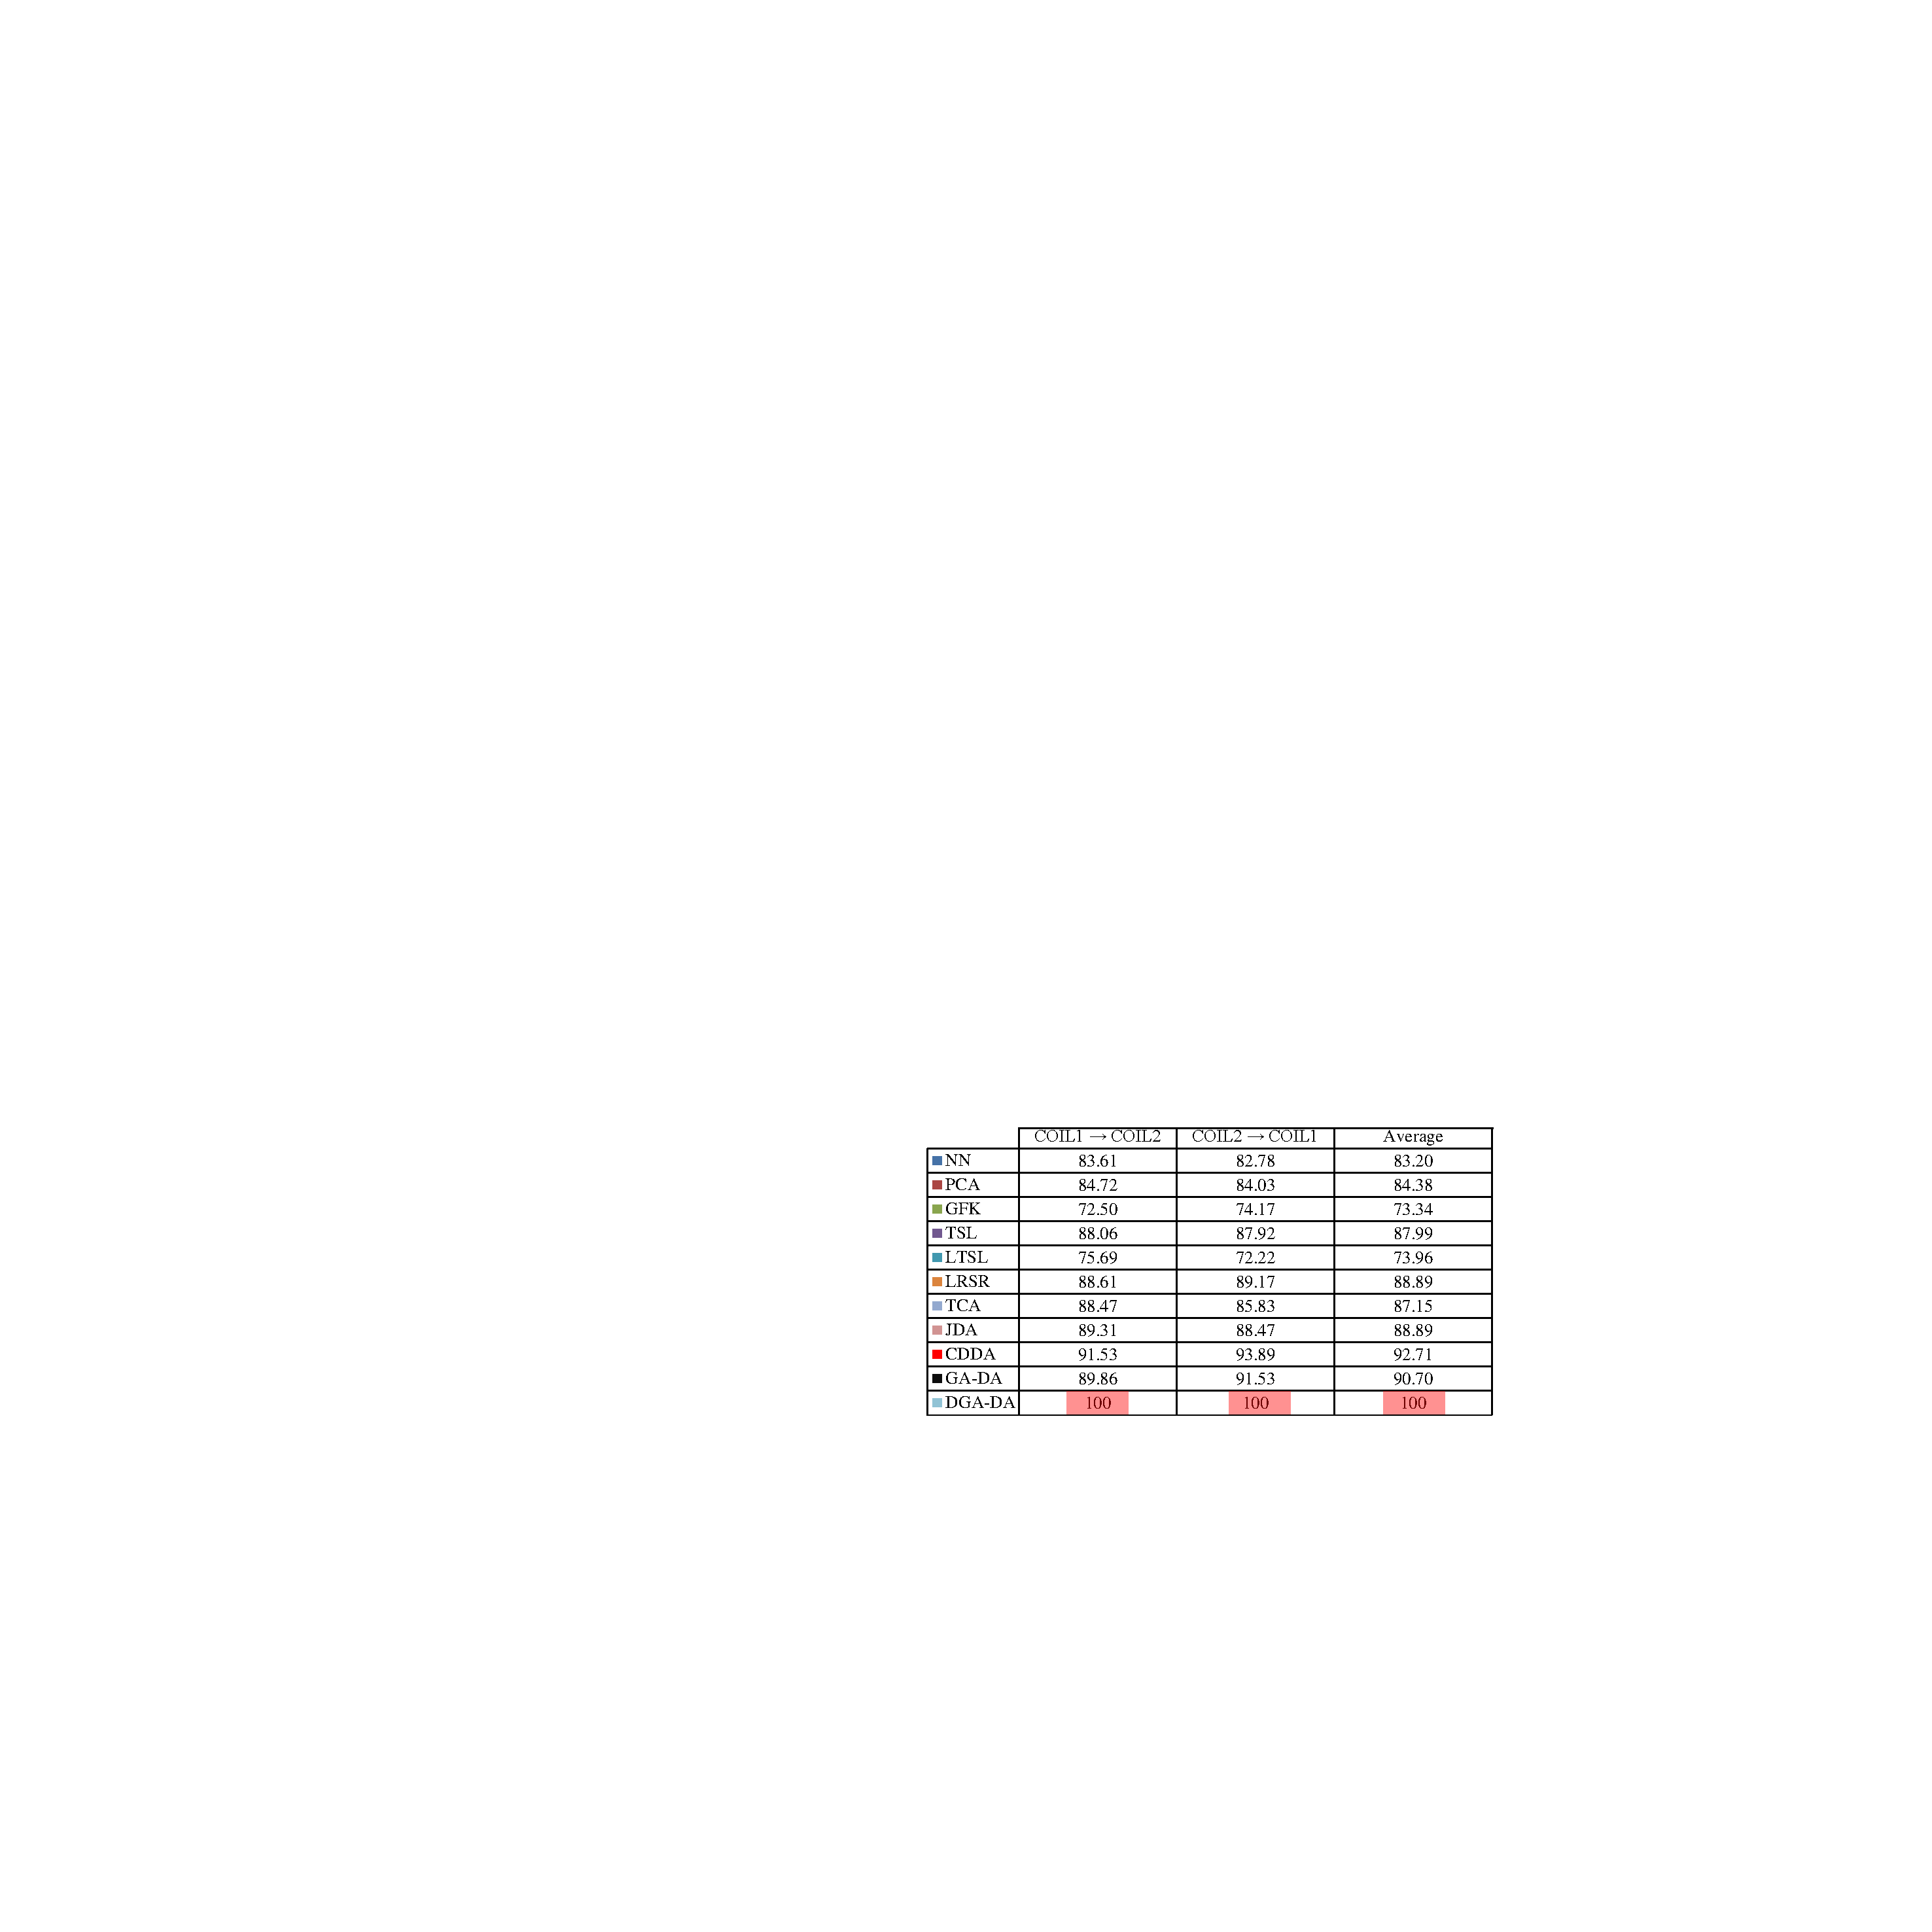
\includegraphics[width=0.9\linewidth]{COIL.pdf}
		%	\vspace{-7pt}
		\caption { Accuracy${\rm{\% }}$ on the COIL Images Dataset.} 
		\label{fig:accCOIL}
	\end{figure} 	
    


\vspace{3pt}
\subsubsection{\textbf{Experiments on the Office+Caltech-256 Data Sets}}
\label{subsubsection:Experiments on the Office+Caltech-256 Data Sets}

	\begin{figure*}[h!]
		\centering
		\includegraphics[width=0.9\linewidth]{DOFFICE.pdf}
		%	\vspace{-7pt}
		\caption { Accuracy${\rm{\% }}$ on the Office+Caltech Images with DeCAF6 Features.} 
		\label{fig:accDO}
	\end{figure*} 	




Fig.\ref{fig:accDO} and Fig.\ref{fig:accSO} synthesize the experimental results in comparison with the state of the art when deep features (\textit{i.e.}, DeCAF6 features) and classic shallow features (\textit{i.e.}, SURE features)   are used, respectively.   

 

% In this part, we present quantitative comparison with stat-of-the-arts in two settings. 
% First, all DA methods are compared  with classical \textit{shallow} features, \textit{i.e.}, SURE features. Second, we also compare with deep learning DA methods, where our feature is deep features. 

\begin{itemize}
\item  As can be seen in Fig.\ref{fig:accSO}, both \textbf{CDDA} and \textbf{DGA-DA} outperform the state of the art method in terms of average accuracy, thereby demonstrating the effectiveness of the proposed DA method. In particular, in comparison with \textbf{JDA} which only cares about data distribution alignment between source and target and the proposed DA method is built upon, \textbf{CDDA} improves \textbf{JDA} by 2 points thanks to the discriminative repulsive force term introduced in our model. When label inference accounts for the underlying data structure, our final model \textbf{DGA-DA} further improves \textbf{CDDA} by roughly 1 point.

% The first scenario's results are presented in Fig.3. where top two ranking places are colored as blue and red respectively. 
% In average, both our CDDA(a) and CDDA(b) outperform the other DA methods, which demonstrates our proposal's effectiveness in transfer knowledge across domains. Especially,  thanks to label deduction constraints, CDDA(b) gains nearly $1\%$ accuracy based on CDDA(a), which proves our assumption on the manifold structure solid. \luo{In addition, the iteration setps between latent susbpace calculation and label propagation as shown in \textbf{Algorithm.1} could design a more solid TL framworks.} Note that JDA can be viewed as a special case of our proposal,  when repulsive force domain adaptation and label propagation are not considered. The setting CDDA(a) enables to quantify the contribution of adding the repulsive force domain adaptation w.r.t. JDA whereas the setting CDDA(b) makes it possible to evidence the contribution of the proposed label propagation in comparison with CDDA(a) and highlight the overall behavior of the proposed method. 

% PCA  doesn't have good results, because it isn't equipped with transfer optimization.   TCA performs better than
% PCA because it jointly performs feature transformation and matching. JDA boosts   performance than previous methods, thanks to  jointly optimizing discrepancies with conditional and marginal distribution. GFK \cite{gong2012geodesic} designs a kernel metric to minimize the divergence of source and target domain. However, the subspace dimension in GFK needs to be small to ensure that the source subspace can transit smoothly along the geodesic flow toward the target subspace \cite{DBLP:journals/tcyb/UzairM17}, which limits the representation ability of GFK. TJM \cite{DBLP:conf/cvpr/LongWDSY14} achieves good performance, it reduces  domain differences by jointly matching  features and constructing new feature representation,  which is invariant to both  distribution difference and  irrelevant instances. The improved accuracy of AELM is attributed to its ability to better represent nonlinear data structure and the feature augmentation. LTSL and LRSR both exploit a unified transform to project  source and target domain into a common subspace. LRSR shows better results than LTSL, because LRSR learns a label relaxed linear classifier, while LTSL selects label randomly. CDML adopts the K-L divergence to measure the similarity of two domains in order to mitigate the disparity across  domains. However, the K-L divergence cannot well align source and target domain and thereby fails to transfer more effective knowledge. In addition, CDML only considers the marginal distribution difference of two domains.

% \luo{ SCA\cite{DBLP:journals/pami/GhifaryBKZ17} defines scatter to measure domain distribution divergence and extract discriminative knowledge between different scatters, however, it unable to well handle label smoothness consistency which designs not so well performance. In Fig.4, our methods achieve the best performance on average accuracy which shows the effectiveness of the proposed method in domain adaptation. As shown in Fig.4, CDDA(b) ranks first accuracy in 12 cross-domain adaptation experiments 2 times and ranks second accuracy 3 times. CDDA(a) ranks second accuracy 5 times. }

	
	\begin{figure*}[h!]
		\centering
		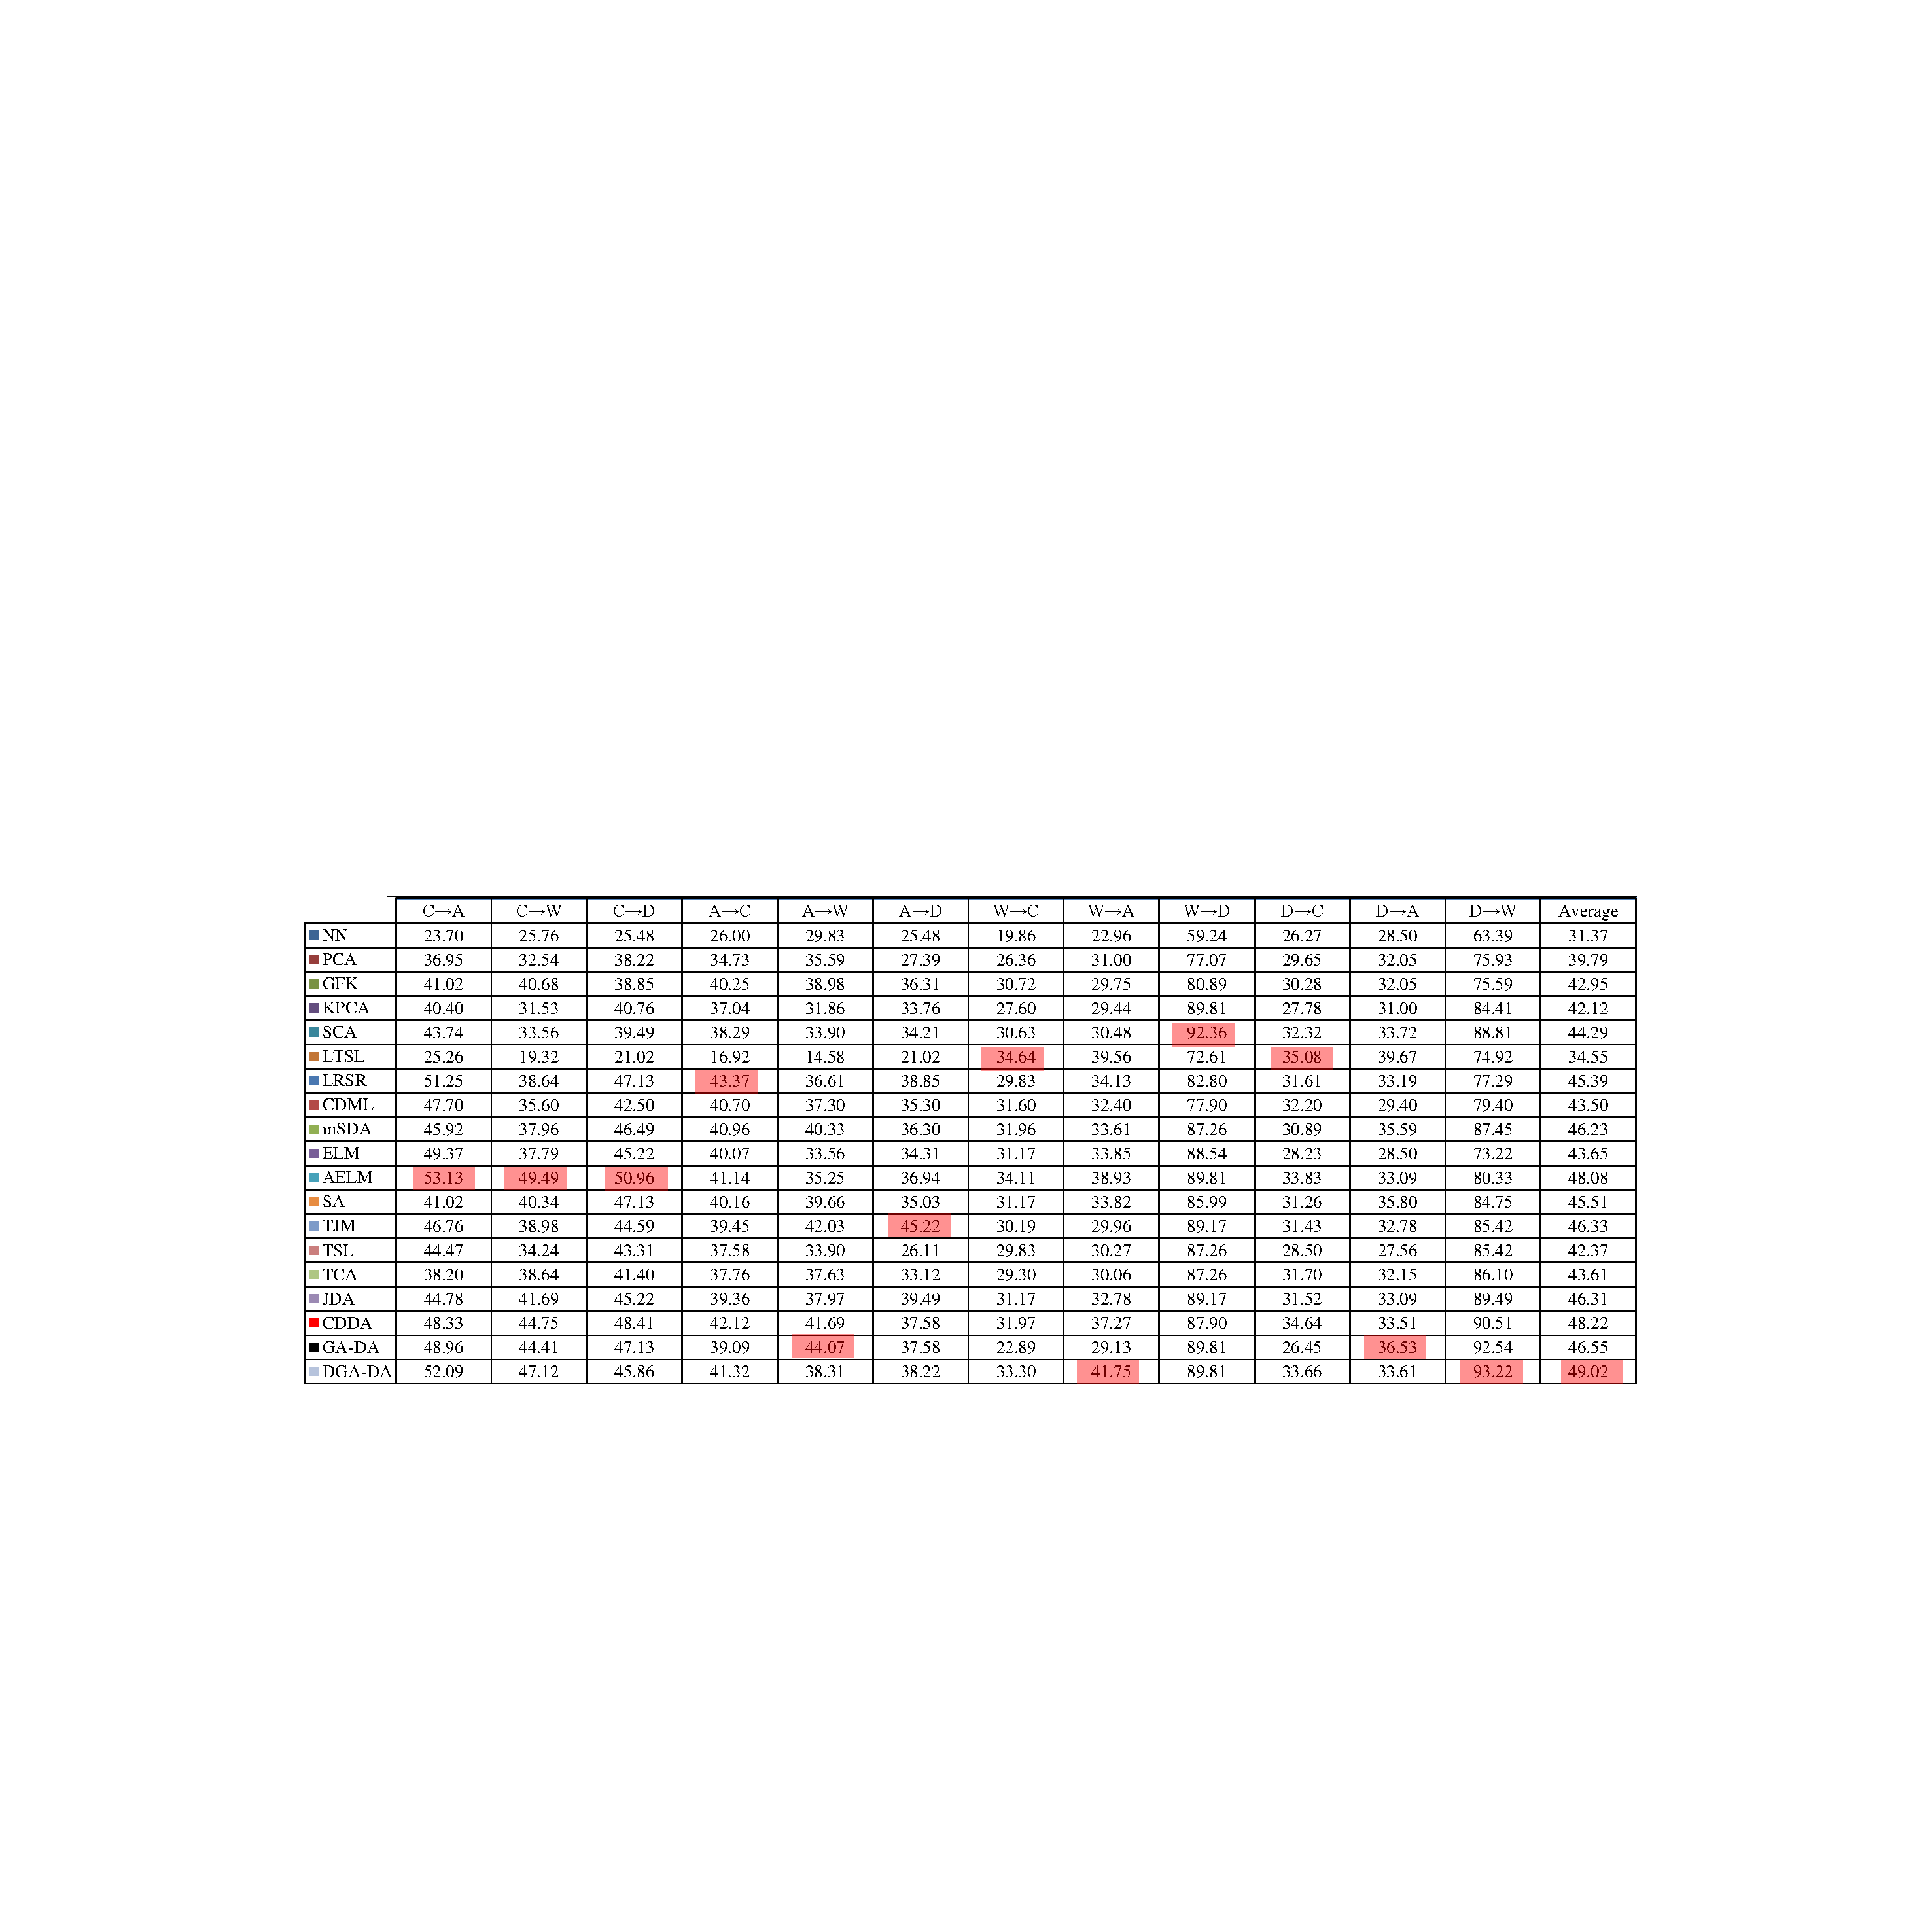
\includegraphics[width=0.9\linewidth]{SOFFICE.pdf}
		%	\vspace{-7pt}
		\caption { Accuracy${\rm{\% }}$ on the Office+Caltech Images with SURF-BoW Features.} 
		\label{fig:accSO}
	\end{figure*} 		




\item Fig.\ref{fig:accDO} compares the proposed DA method using deep features \textit{w.r.t.}   the state of the art, in particular end-to-end deep learning-based DA methods. As can be seen in Fig.\ref{fig:accDO}, the use of deep features has enabled impressive accuracy improvement over shallow features. Simple baseline methods, \textit{e.g.}, \textbf{NN}, \textbf{PCA}, see their accuracy soared by roughly 40 points, demonstrating the power of deep learning paradigm. Our proposed DA method also takes advantage of this jump and sees its accuracy soared from 48.22 to 89.13 for \textbf{CDDA} and from 49.02 to 90.43 for \textbf{DGA-DA}. As for shallow features, \textbf{CDDA} improves \textbf{JDA} by 3 points and \textbf{DGA-DA} further ameliorates \textbf{CDDA} by 1 point when label inference accounts for the underlying data geometric structure. As a result, \textbf{DGA-DA} displays the best average accuracy and outperforms slightly \textbf{DAN}.   
% are shown in Fig.4. We could observe that all the methods achieve better results using DeCAF6 \cite{DBLP:conf/icml/DonahueJVHZTD14} instead of  SURF\cite{gong2012geodesic} . This demonstrates the impressive representation ability of  deep features. More specifically, AlexNet\cite{krizhevsky2012imagenet}, DAN\cite{long2015learning} and DDC\cite{DBLP:journals/corr/TzengHZSD14} are state-of-the-art deep learning based approach for DA. \luo{Follow the similar setting as RTN\cite{long2016unsupervised}, we implement all deep methods(AlexNet, DAN, RTN) based on the Caffe deep-learning framework, and fine-tune from Caffe-provided models of AlexNet pre-trained on ImageNet. AlexNet results is considered as \textbf{baseline results}. DAN further improve TL performance due to it regularizes each full connected layer for matching cross-domain data.} RTML\cite{DBLP:journals/tip/DingF17} is based on metric learning which exploits knowledge transfer to mitigate the domain shift in both sample space and feature space. \luo{JGSA is a powerful method which leaverages domain/subdomain variations and distribution shift to design a discriminative optimization model, however, which could extract a more robust common latent subspace if it considers to preserve manifold structure simultaneously.}  With the repulsive force integrated and NN as label predictor, CDDA(a) outperforms JDA on 10 cross-domain tasks out of 12 and improves JDA's overall average accuracy by roughly 3 points, thereby demonstrating the effectiveness of the proposed repulsive force domain adaptation. Now, in adopting the proposed label propagation under the constraint of both label smoothness and geometric structure consistency, CDDA(b) further improves CDDA(a) by roughly 1 points in terms of overall average accuracy and outperforms JDA by more than 4 points. As can be seen in Fig.5,  \textbf{CDDA(b)} as represented by the red curve is on the top of the other curves along  the axis of 12 cross-domain image classification tasks. 


% In Fig.5, our methods rank first(CDDA(b)) and third(CDDA(a)) performance on average accuracy which shows the effectiveness of the proposed method in domain adaptation. As shown in Fig.5, CDDA(b) ranks first accuracy in 12 cross-domain adaptation experiments 7 times and ranks second accuracy 2 times. CDDA(a) ranks first accuracy in 12 cross-domain adaptation experiments 5 times and ranks second accuracy 1 times. Moreover, CDDA(a) and CDDA(b) are only two methods which achieves full accuracy ($100\% $) both in cases, e.g.,  \emph{W} $\rightarrow$ \emph{D} $ and $ \emph{D} $\rightarrow$ \emph{W}.


% \item \luo{As shown in Fig.4 and Fig.5, the transfer learning perfromance of CDDA would be highly improved through increasing the quality of features. It is important to emphasize that the proposed CDDA method is not a feature extraction technique but a DA technique. The perfromance of CDDA could be imporved if we extract more efficient features. }


\end{itemize}
    
    
    
% \subsubsection{\textbf{Experiments on the COIL 20 Dataset \textcolor{red}{This achieved 100 perfromance in DGA-DA} }} 
% \label{subsubsection: results on the COIL dataset}
% The COIL dataset (see fig.\ref{fig:data}) features the challenge of pose variations between the source and target domain. Fig.\ref{fig:accCOIL} depicts the experimental results on the COIL dataset. As can be seen in this figure, the proposed CDDA and DGA-DA depicts an overall average accuracy of  $\bf 92.71\%$ and \textcolor{red}{$\bf 100.00\%$}, respectively. They both outperform the eight baseline DA algorithms with a large margin.

% It is worth noting that, when performing label deduction based on the underlying data manifold structure, the proposed DGA-DA improves its sibling CDDA by a margin as high as roughly 7 points, thereby highlighting the importance of data geometry aware label inference as introduced in DGA-DA. As compared to JDA, the proposed CDDA, which adds a discriminative \textit{repulsive force} term \textit{w.r.t.} JDA, also shows its effectiveness and improves the latter by more than 3 points. 

% % \begin{itemize}	
% % \item As can be seen in Fig.5 , the proposed CDDA depicts an overall average accuracy of  $\bf 92.71\%$ and $\bf 99.65\%$, respectively,  with respect to the above two settings. They both outperform the eight baseline algorithms with a large margin.

% % \item CDDA(b) achieves 6.94${\rm{\% }}$ accuracy improvements compare with CDDA(a) owning to the merits of label deduction constraints. The improvements prove that iteration steps between latent subspace calculation and label deduction could design a more representative subspace.

% % \item  It is worth noting  that the proposed  CDDA(b) depicts $\bf 99.65$ accuracy on \textbf{COIL20}; This is rather an unexpected impressive score given the unsupervised nature of the domain adaptation for the target domain with non-deep features.
% % \end{itemize}





% 	\begin{figure}[h!]
% 		\centering
% 		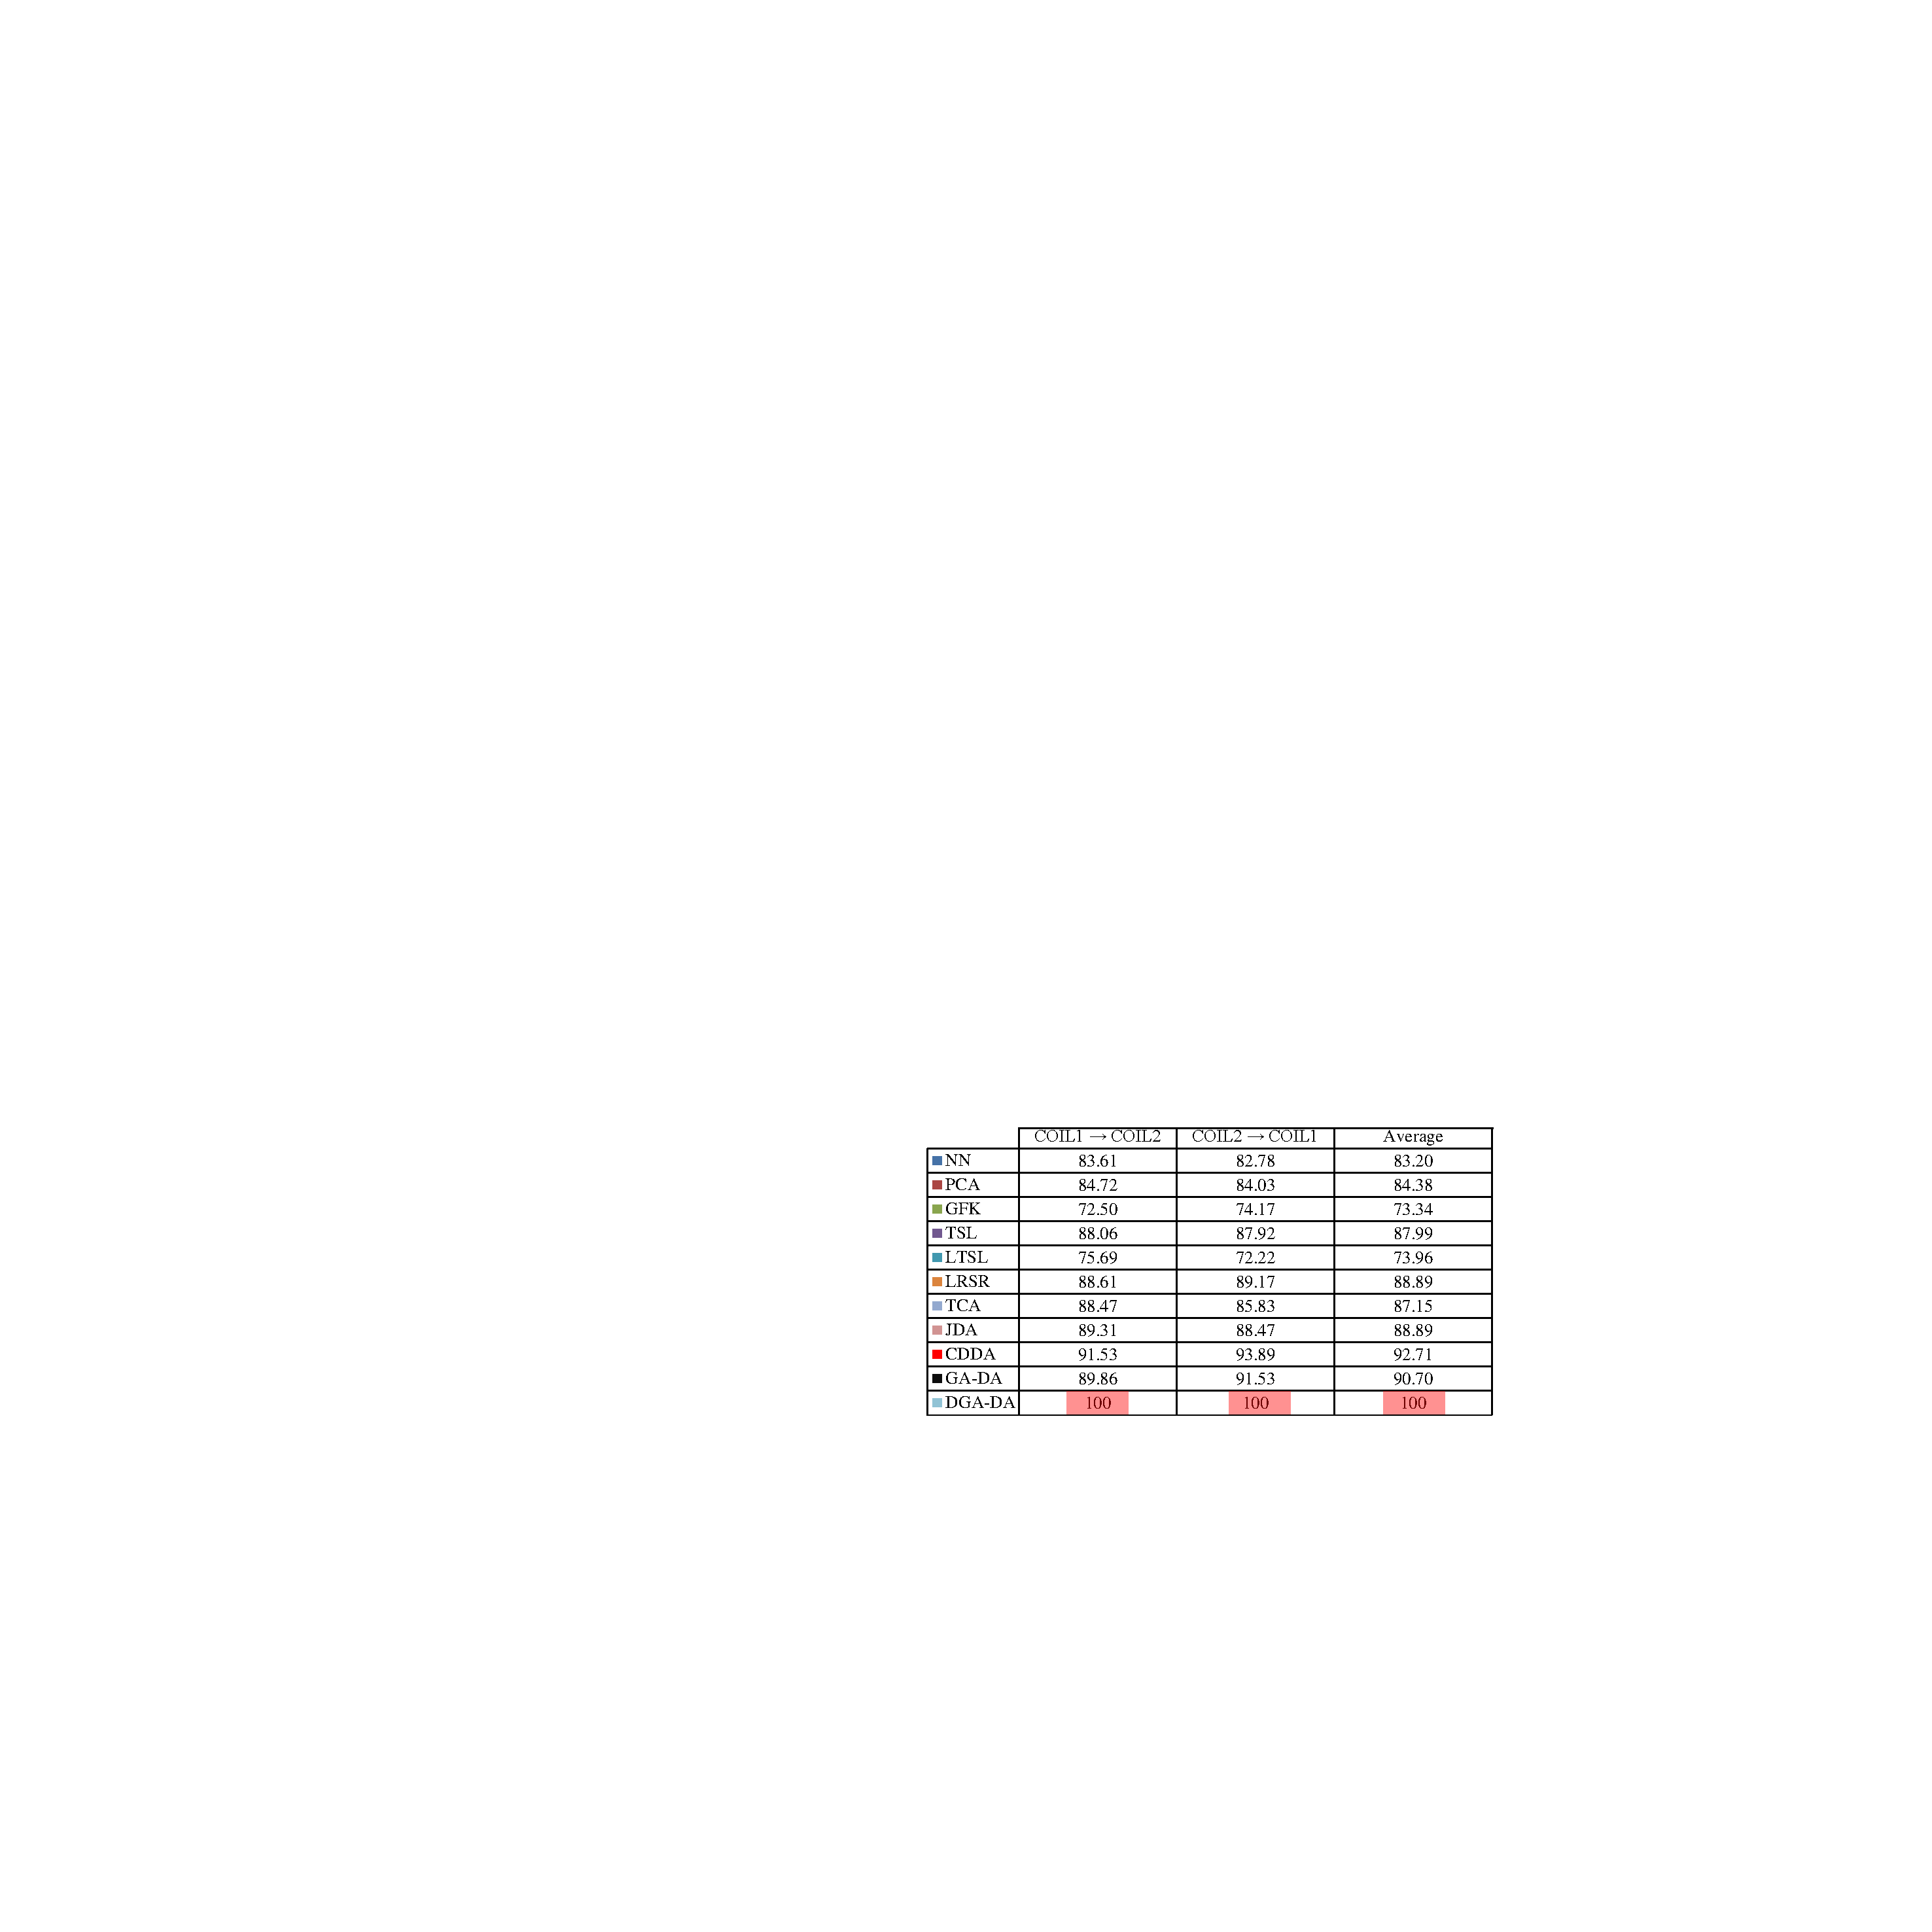
\includegraphics[width=1\linewidth]{COIL.pdf}
% 		%	\vspace{-7pt}
% 		\caption { Accuracy${\rm{\% }}$ on the COIL Images Dataset.} 
% 		\label{fig:accCOIL}
% 	\end{figure} 	
    

    
\subsubsection{\textbf{Experiments on the USPS+MNIST Data Set}}
\label{subsubsection: experiments on the UPS+MNIST Datasets}
The UPS+MNIST dataset features different writing styles between source and target. Fig.\ref{fig:accUSPS} lists the experimental results in comparison with 14 state of the art DA methods. As can be seen in the table, \textbf{CDDA} displays a 69.14\% average accuracy and ranks the third best performer. It shows its effectiveness once more as it improves its baseline \textbf{JDA} by more than 5 points on average. When accounting for the underlying data geometry structure, the proposed \textbf{DGA-DA} further improves its sibling \textbf{CDDA} by a margin more than 7 points and displays the state of the art performance of a 76.54\% accuracy. It is worth noting that the second best DA performer on this dataset, \textit{i.e.}, \textbf{JGSA}, also suggests aligning both statistically and geometrically data, and thereby corroborates our data geometry aware DA approach.       

	\begin{figure}[h!]
		\centering
		\includegraphics[width=0.8\linewidth]{USPS.pdf}
		%	\vspace{-7pt}
		\caption { Accuracy${\rm{\% }}$ on the USPS+MNIST Images Dataset.} 
		\label{fig:accUSPS}
	\end{figure} 	


% \begin{itemize}	
% 	\item Fig.7 summarizes the classification accuracy on the USPS
% 	+MNIST dataset. Compare with other 14 DA methods, CDDA(b) and CDDA(a) rank first and third classification accuracy respectively.
	
% 	\item JGSA achieve higher performance compare with CDDA(a) since which jointly considers domain/sub-domain variation and domain shift simultaneously. JGSA successfully extract discriminative knowledge between target domain and source domain, however, which could design a more efficient common latent subspace if  it well considers data manifold structure similar as CDDA(b).


% \end{itemize}



\subsubsection{\textbf{Experiments on the CMU PIE Data Set}}
\label{subsubsection:Experiments on the CMU PIE dataset}

The CMU PIE dataset is a large face dataset featuring both illumination and pose variations. Fig.\ref{fig:accPIE} synthesizes the experimental results for DA using this dataset. As can be seen in the figure, similarly as in the previous experiments, the proposed \textbf{DGA-DA} displays the best average accuracy over 20 cross-domain adaptation experiments. In aligning both marginal and conditional data distributions, \textbf{JDA} performs quite well and displays a 60.24\% average accuracy. In integrating the discriminative repulsive force term, \textbf{CDDA} improves \textbf{JDA} by roughly 3 points. \textbf{DGA-DA} further ameliorates \textbf{CDDA} by more than 1 point.   

% Specifically, as shown in Fig.8, CDDA(b) ranks first accuracy in 20 cross-domain adaptation experiments 8 times and ranks second accuracy 7 times. CDDA(a) ranks first accuracy in 20 cross-domain adaptation experiments 4 times and ranks second accuracy 6 times.

It is interesting to note that the second best performer on this dataset, namely \textbf{LRSR}, also tries to align geometrically source and target data through both low rank and sparse constraints so that source and target data are interleaved within a novel shared feature subspace. 

% As shown in Fig.8, LRSR ranks second in average accuracy. LTSL superficially seems to be similar to LRSR. Both methods propose a unified transform to drag source domain and target domain into a common subspace. However, LRSR outperforms LTSL mainly because LRSR uses the sparse constraint to capture the local structure among the source and target domains. RDALR is another method similar as LRSR, both of them introduce sparse reconstruction and low-rank constraint in optimization model. However, RDALR neglects one aspect is that when the source domain data are transformed into the target domain, the data of different subjects may overlap each other so that they cannot be separated. Moreover, LRSR introduce a smart	transformation matrix\cite{xiang2012discriminative} which has more freedom to make the source domain and target domain closer enough to each other owning to the label relaxation.

    
	\begin{figure*}[h!]
		\centering
		\includegraphics[width=1\linewidth]{PIE.pdf}
		%	\vspace{-7pt}
		\caption { Accuracy${\rm{\% }}$ on the PIE Images Dataset.} 
		\label{fig:accPIE}
	\end{figure*} 	

% \begin{itemize}	
% 	\item The CMU PIE data set is a large data set. The experiment results about DA test on PIE are shown in Fig.8. Again, our method performs best results in average accuracy over 20 cross-domain adaptation experiments. Specifically, as shown in Fig.8, CDDA(b) ranks first accuracy in 20 cross-domain adaptation experiments 8 times and ranks second accuracy 7 times. CDDA(a) ranks first accuracy in 20 cross-domain adaptation experiments 4 times and ranks second accuracy 6 times.
	
% 	\item As shown in Fig.8, LRSR ranks second in average accuracy. LTSL superficially seems to be similar to LRSR. Both methods propose a unified transform to drag source domain and target domain into a common subspace. However, LRSR outperforms LTSL mainly because LRSR uses the sparse constraint to capture the local structure among the source and target domains. RDALR is another method similar as LRSR, both of them introduce sparse reconstruction and low-rank constraint in optimization model. However, RDALR neglects one aspect is that when the source domain data are transformed into the target domain, the data of different subjects may overlap each other so that they cannot be separated. Moreover, LRSR introduce a smart	transformation matrix\cite{xiang2012discriminative} which has more freedom to make the source domain and target domain closer enough to each other owning to the label relaxation.
% 	\end{itemize}




\subsection{Convergence and Parameter Sensitivity }
\label{subsection: Convergence and Parameter Sensitivity}



\begin{figure*}[h!]
		\begin{center}
			\begin{tabular}{c}
	\includegraphics[width=0.95\linewidth]{k.pdf}
			\end{tabular}
		\end{center}
        	\vspace{-10pt} 
		\caption {Sensitivity analysis of the proposed methods:  (a) accuracy \textit{w.r.t.} subspace dimension  $k$ of CDDA; (b)accuracy \textit{w.r.t.} subspace dimension $k$ of GA-DA;
(c) accuracy \textit{w.r.t.} subspace dimension $k$ of DGA-DA.
Four datasets are used, \textit{i.e.}, COIL1, COIL2, USPS and MNIST.} 
        		\label{fig:k}
	\end{figure*} 


\begin{figure}[h!]
	\centering
	\includegraphics[width=0.9\linewidth]{parameter.pdf}
	\caption {The classification accuracies of the proposed \textbf{GA-DA} and \textbf{DGA-DA} method vs. the parameters $\alpha $ and $\lambda $ on the selected four cross domains data sets, \textit{i.e.}, DSLR (D), Webcam (W), COIL1 and COIL2, with $k$ held fixed at $100$. } 
    	\label{fig:para}
\end{figure} 



\begin{figure*}[h!]
	\centering
	\includegraphics[width=0.94\linewidth]{iteration.pdf}
	\caption {Convergence analysis using 12 cross-domain image classification tasks on Office+Caltech256 datasets with DeCAF6 Features. (accuracy w.r.t $\#$iterations) } 
    	\label{fig:accITER}
\end{figure*} 



\begin{figure}[h!]
	\centering
	\includegraphics[width=1\linewidth]{compare.pdf}
	\caption {Comparisons of baseline domain adaptation methods and the proposed \textbf{CDDA}, \textbf{GA-DA} and \textbf{DGA-DA} method on the synthetic data} 
    	\label{fig:compare}
\end{figure} 





\begin{figure*}[h!]
	\centering
	\includegraphics[width=0.95\linewidth]{VI.pdf}
	\caption {Accuracy(${\rm{\% }}$) and Visualization results of the MNIST$\rightarrow$USPS DA task. Fig.\ref{fig:vi}(a), Fig.\ref{fig:vi}(b) and Fig.\ref{fig:vi}(c) are visualization results of MNIST, USPS,  MNIST$\& $USPS datasets in their \textbf{Original} data space, respectively. After domain adaptation, Fig.\ref{fig:vi}(d), Fig.\ref{fig:vi}(e), Fig.\ref{fig:vi}(f) and Fig.\ref{fig:vi}(g) visualize the MNIST$\& $USPS datasets in \textbf{JDA}, \textbf{CDDA}, \textbf{GA-DA} and \textbf{DGA-DA} subspaces, respectively. Fig.\ref{fig:vi}(h), Fig.\ref{fig:vi}(i), Fig.\ref{fig:vi}(j) and Fig.\ref{fig:vi}(k) show the visualization results of the target domain USPS in \textbf{JDA}, \textbf{CDDA}, \textbf{GA-DA} and \textbf{DGA-DA} subspaces, respectively. The ten digit classes are represented by different colors.}  
    	\label{fig:vi}
\end{figure*} 



While the proposed \textbf{DGA-DA} displays state of the art performance over 36 DA tasks through six datasets (USPS, MINIST, COIL20, PIE, Amazon, Caltech), an important question is how fast the proposed method converges (sect.\ref{subsubsection: Convergence analysis}) as well as its sensitivity \textit{w.r.t.} its hyper-parameters (Sect.\ref{subsubsection: Parameter sensitivity}). 

\subsubsection{Parameter sensitivity}
\label{subsubsection: Parameter sensitivity}
	
Three hyper-parameters, namely  $k$, $\lambda$ and $\alpha$, are introduced in the proposed methods.  $k$ is the dimension of the extracted feature subspace which determines the structure of low-dimension embedding. In Fig.\ref{fig:k}, we plot the classification accuracies of the proposed DA method \textit{w.r.t} different values of $k$ on the  \textbf{COIL} and \textbf{USPS+MINIST} datasets. As shown in Fig.\ref{fig:k}, the subspace dimensionality $k$ varies with $k  \in \{20,40,60,80,100,120,140,160,180,200\}$, yet the proposed 3 DA variants, namely, \textbf{CDDA}, \textbf{GA-DA} and \textbf{DGA-DA}, remain stable \textit{w.r.t.}  a wide range of with $k \in \{ 40 \le k  \le 200\} $. In our experiments,  we set $k = 100$ to balance efficiency and accuracy.



$\lambda$ as introduced in Eq.(\ref{eq:final model}) and Eq.(\ref{eq:prob1}) aims to regularize the projection matrix $\textbf{A}$ to avoid over-fitting the chosen shared feature subspace with respect to both source and target data.  $\alpha {\rm{ = }}\frac{1}{{1 + \mu }}$ as defined in Eq.(\ref{eq:Y_alpha_optimal}) is a trade-off parameter which balances  LSC and GSC. We study the sensitivity of the proposed \textbf{GA-DA} and \textbf{DGA-DA} methods with a wide range of parameter values, \textit{i.e.}, $\alpha  = (0.0001,0.001,0.01,0.1,0.5,0.9,0.99)$ and $\lambda  = (0.0001,0.001,0.01,0.1,1,10,100)$. We plot in Fig.\ref{fig:para} the results on \emph{D} $\rightarrow$ \emph{W} $ and $ \emph{COIL1} $\rightarrow$ \emph{COIL2} datasets on both methods with $k$ held fixed at $100$. As can be seen from Fig.\ref{fig:para}, the proposed \textbf{GA-DA} and \textbf{DGA-DA} display their stability as the resultant classification  accuracies remain roughly the same despite  a wide range of $\lambda $ and $\alpha $ values. 

\subsubsection{Convergence analysis}
\label{subsubsection: Convergence analysis}


In Fig.\ref{fig:accITER}, we further perform  convergence analysis of the proposed  \textbf{CDDA}, \textbf{GA-DA} and \textbf{DGA-DA} methods  using the \textbf{DeCAF6} features on the \textbf{Office+Caltech} datasets. The question here is how fast a DA method achieves its best performance \textit{w.r.t.} the number of iterations $T$.
Fig.\ref{fig:accITER} reports 12 cross domain adaptation experiments ( \emph{C} $\rightarrow$ \emph{A}, \emph{C} $\rightarrow$ \emph{W} ... \emph{D} $\rightarrow$ \emph{A} , \emph{D} $\rightarrow$ \emph{W}  ) with the number of iterations $T = (1,2,3,4,5,6,7,8,9,10)$. 
 
As shown in Fig.\ref{fig:accITER},  \textbf{CDDA}, \textbf{GA-DA} and \textbf{DGA-DA} converge within 3$ \sim $5 iterations during optimization.
% It worth noting that,  \textbf{DGA-DA} and \textbf{GA-DA} shows more fast convergence than \textbf{CDDA}, this could be witness on Fig.\ref{fig:accITER}(e), Fig.\ref{fig:accITER}(h) and Fig.\ref{fig:accITER}(k). The main reason is aware of manifold structure preservation induce more efficient convergence.




%\subsubsection{Convergence analysis}
%\label{subsubsection: Convergence analysis}

%Since a serious previous research\cite{Zhang_2017_CVPR,DBLP:conf/cvpr/LongWDSY14,long2015learning,DBLP:journals/tip/DingF17,DBLP:journals/pami/GhifaryBKZ17} achieve higher performance on \textbf{DeCAF6} features comapre with \textbf{SURF} features. Here we check the  convergence performance of our proposed CDDA in different iterations with extracted \textbf{DeCAF6} features on \textbf{Office+Caltech} datasets. With out loss of generality, we propose convergence analysis on \textbf{Office+Caltech} datasets and \textbf{COIL20} datasets with extracted \textbf{SURF} features. We also give JDA's convergence performance used to compare with CDDA since JDA could be viewed as special case of the proposed CDDA method. Similar trends can be observed on all the other datasets.


%The accuracy w.r.t. $\#$iterations is shown in Fig.9 and Fig.10 (a). Fig.9 shows 24 cross domain adaptation experiments( \emph{C} $\rightarrow$ \emph{A}, \emph{C} $\rightarrow$ \emph{W} ... \emph{D} $\rightarrow$ \emph{A} , \emph{D} $\rightarrow$ \emph{W}  ) which test on \textbf{Office+Caltech} datasets with deep features. Fig.9 shows both CDDA(a) and CDDA(b) converged within 5$ \sim $10 iterations during optimization. CDDA(b) shows more fast convergence than CDDA(a), this could be witness on Fig.9(b), Fig.9(c) and Fig.9(e).




%Moreover, convergence analysis about \emph{COIL2} $\rightarrow$ \emph{COIL1} and  \emph{C} $\rightarrow$ \emph{W} with extracted \textbf{SURF} features  is proposed in Fig.9(a). In addition, we give JDA's results as base line for comparison. Fig.9(a) shows CDDA(b) gain the best convergence speed, especially in  \emph{COIL2} $\rightarrow$ \emph{COIL1} CDDA(b) converged at the first iteration.


%\subsubsection{Parameter sensitivity}
%\label{subsubsection: Parameter sensitivity}
								
%In the experiment, CDDA have two settings: two parameters ($k$ and $\lambda$) in \textbf{CDDA(a)} and three ($k$, $\lambda$ and $\alpha$) in  \textbf{CDDA(b)}. 

%Firstly, we ran \textbf{CDDA(b)} with varying values of $\alpha$ to test its performance. The parameter $\alpha$ defined in Eq.(\ref{eq:Y_optimal}) specifies the relative amount of the information from its neighbors and its initial label information. We evaluate different combinations of values selected from a reasonable discrete set $\alpha {\rm{ = \{ 1}}{{\rm{0}}^2},10,0.99,1{0^{{\rm{ - }}1}},1{0^{{\rm{ - }}2}},1{0^{{\rm{ - 3}}}}{\rm{\} }}$  on  \emph{COIL2} $\rightarrow$ \emph{COIL1} and  \emph{C} $\rightarrow$ \emph{W}. As shown Fig.10 (b), which indicates \textbf{ CDDA(b)} achieves the best performance when $\alpha$ is close to 0.99 on \emph{COIL2} $\rightarrow$ \emph{COIL1} and the performance is stable  when  $\alpha$ is less than 0.99. \textbf{ CDDA(b)} also achieves well performance when $\alpha$ is $\alpha  \le 0.99$.  However, $\alpha$ could not be stable if we select different datasets, since the data distribution may share huge differences. Given a novel dataset, we tune the parameter $\alpha$ in the range  [0.001,1]. For instance, in the \textbf{PIE} database, we set the optimal $\alpha$  to 0.2. 

%$\lambda$ is the regularization parameter defined in \textbf{CDDA}, which proposed to guarantee the optimization problem to be well-defined. The first optimization sub-problem described in Eq.(\ref{eq:ours_math}) could be ill-defined with $\lambda  \approx 0$.  We plot classification accuracy w.r.t different value of $\lambda$ in Fig.11, which proposed on COIL20, USPS+MINIST datasets. \textbf{CDDA(a)} achieves well performance on \emph{COIL1} $\rightarrow$ \emph{COIL2} and \emph{COIL2} $\rightarrow$ \emph{COIL1} with $\lambda  \in \{ 0.01 \le \lambda  \le 100\} $, while works well on  \emph{USPS} $\rightarrow$ \emph{MNIST} and \emph{MNIST} $\rightarrow$ \emph{USPS} with $\lambda  \in \{ 0.1 \le \lambda  \le 10\} $. \textbf{CDDA(b)} shows well performance on \emph{COIL1} $\rightarrow$ \emph{COIL2} and \emph{COIL2} $\rightarrow$ \emph{COIL1} with $\lambda  \in \{ 0.0001 \le \lambda  \le 100\} $, while works on \emph{USPS} $\rightarrow$ \emph{MNIST} and \emph{MNIST} $\rightarrow$ \emph{USPS} same as \textbf{CDDA(a)}. In this experiment we set $\lambda  \in \{ 0.1 \le \lambda  \le 10\} $.
						

%In \textbf{CDDA}, $k$ represents dimension of extracted latent subspace, which determines the structure of dimension reduction. We plot classification accuracy w.r.t different value of $k$ in Fig.12 with proposed \textbf{COIL20}, \textbf{USPS+MINIST} datasets. After analysis Fig.12, both \textbf{CDDA(a)} and \textbf{CDDA(b)} could achieve well performance with $k \in \{ 40 \le k  \le 200\} $ on both datasets. In this experiment, we could choose $k$ in a large rang $k \in [40,200]$. However, experiment could be more complex and time consuming with $k$ getting larger. To balance efficiency and accuracy we set $k = 100$.




\subsection{Analysis and Verification}
\label{subsection:Analysis and Verification}



To further gain insight of the proposed \textbf{CDDA}, \textbf{GA-DA} and \textbf{DGA-DA} \textit{w.r.t.} its domain adaptation skills, we also evaluate the proposed methods using a synthetic dataset in comparison with several state of the art DA methods. Fig.\ref{fig:compare} visualizes the original data distributions with 4 classes and the resultant shared feature subspaces as computed by \textbf{TCA}, \textbf{JDA}, \textbf{TJM}, \textbf{SCA}, \textbf{CDDA}, \textbf{GA-DA} and \textbf{DGA-DA}, respectively. In this experiment, we focus our attention on the ability of the DA methods to: :  (a) narrow the discrepancies of data distributions between source and target; (b) increase data discriminativeness; and (c) align data geometric structures between source and target. As such, the original synthetic data depicts slight distribution discrepancies between source and target for the first two class data, wide distribution mismatch for the third and fourth class data. Fourth class data further depict a moon like geometric structure. 




As can be seen in Fig.\ref{fig:compare}, baseline methods, \textit{e.g.}, \textbf{TCA}, \textbf{SCA}, \textbf{TJM} have difficulties to align data distributions with wide discrepancies, \textit{e.g.}, third class data. \textbf{JDA} narrow data distribution discrepancies but lacks class data discriminativeness. The proposed variant \textbf{CDDA} ameliorates \textbf{JDA} and makes class data well separated thanks to the introduced \textit{repulsive force} term but falls short to preserve data geometric structure (see the fourth  moon like class data. The variant \textbf{GA-DA} align data distributions and preserves the underlying data geometric structures thanks to label smoothness consistency (LSC) and geometric structure consistency (GSC) but lacks data discriminativeness. In contrast, thanks to the joint consideration of data discriminativeness and geometric structure awareness, the proposed \textbf{DGA-DA} not only align data distributions compactly but also separate class data very distinctively. Furthermore, it also preserves the underlying data geometric structures.   

		

% In this paper, we design three DA methods, \textit{e.g.}, \textbf{CDDA}, \textbf{GA-DA} and \textbf{DGA-DA}. \textbf{DGA-DA} improves \textbf{CDDA} via jointly aware geometric structure constraints (GSC and LSC), and improves \textbf{GA-DA} via adding distinctive DA constraints compare with traditional probabilistic approximate DA methods\cite{pan2011domain,long2013transfer}. 






The above findings can be further verified using real data through the MNIST$\rightarrow$USPS DA task  where the proposed DA methods achieves remarkable results (See Fig.\ref{fig:accUSPS}). Fig.\ref{fig:vi} visualizes class explicit data distributions in their original subspace and  the resultant shared feature subspace using \textbf{JDA} and the three variants of the proposed DA method, namely \textbf{CDDA}, \textbf{GA-DA} , \textbf{DGA-DA}, with the same experimental setting. 

% over the cross-domain dataset, namely \emph{MNIST} $\rightarrow$ \emph{USPS}. Different colors represent different classes.
% \textbf{JDA} and proposed  \textbf{CDDA}, \textbf{GA-DA} , \textbf{DGA-DA} with same experimental settings and they are benchmarked using the popular USPS+MNIST dataset. Fig.\ref{fig:vi} plots these experimental results. To gain intuition, Fig.\ref{fig:vi} further visualizes class explicit data distributions in their original subspace and calculated the resultant shared feature subspace using JDA and the three proposed methods over the cross-domain dataset, namely \emph{MNIST} $\rightarrow$ \emph{USPS}. Different colors represent different classes.

% One interesting question is how each of these constraints contribute to the final model Eq.(\ref{eq:final model}). For this purpose we compare \textbf{JDA} and proposed  \textbf{CDDA}, \textbf{GA-DA} , \textbf{DGA-DA} with same experimental settings and they are benchmarked using the popular USPS+MNIST dataset. Fig.\ref{fig:vi} plots these experimental results. To gain intuition, Fig.\ref{fig:vi} further visualizes class explicit data distributions in their original subspace and calculated the resultant shared feature subspace using JDA and the three proposed methods over the cross-domain dataset, namely \emph{MNIST} $\rightarrow$ \emph{USPS}. Different colors represent different classes.
 


\begin{itemize}
	
	\item Data distributions and geometric structures. Fig.\ref{fig:vi}(a,b,c) visualize the MNIST, USPS,  MNIST$\& $USPS datasets in their \textbf{Original} data space, respectively. As shown in these figures, the MNIST and USPS datasets depict different data distributions and various data structures. In particular, yellow  dots represent digit 2. They show a long and narrow shape in MNIST (Fig.\ref{fig:vi}(a)) while a circle like shape in USPS (Fig.\ref{fig:vi}(b)). They further display large data discrepancies across domain (Fig.\ref{fig:vi}(c)) as for all the other classes.
	
	
    \item Contribution of the \textit{repulsive force} term. Visualization results in Fig.\ref{fig:vi}(h,i,j,k) show that, in comparison with their respective baseline DA methods, \textit{i.e.}, \textbf{JDA} (Fig.\ref{fig:vi}(h)) and \textbf{GA-DA} (Fig.\ref{fig:vi}(j)), the proposed two DA variants, \textit{i.e.}, \textbf{CDDA}(Fig.\ref{fig:vi}(i))  and \textbf{DGA-DA}(Fig.\ref{fig:vi}(k)) which integrate in their model the \textit{repulsive force} term as introduced in Sect.\ref{subsubsection:Discriminative DA}, achieve data discriminativeness in compacting intra-class instances and separating inter-class data, respectively. As a result,  as shown in Fig.\ref{fig:accUSPS}, \textbf{DGA-DA} outperforms \textbf{GA-DA} by ${\bf 6.94}\uparrow$ points, and \textbf{CDDA} outperforms \textbf{JDA} by ${\bf 8.94}\uparrow$ points,respectively, thereby illustrating the importance of increasing data discriminativeness in DA. 
     
      
    
    

    \item Contribution of Geometric Structure Awareness. Visualization results in Fig.\ref{fig:vi}(d,e) show that the \textbf{JDA} and \textbf{CDDA}'s subspaces fail to preserve the geometric structures of the underlying data manifold. For instance, the long and narrow shape of the orange dots in the source MNIST domain and the corresponding circle blob orange cloud in the target USPS domain (Fig.\ref{fig:vi}(c)) are not preserved anymore in the \textbf{JDA} (Fig.\ref{fig:vi}(d)) and \textbf{CDDA} (Fig.\ref{fig:vi}(e)) subspaces. In contrast, thanks to the geometry awareness constraints, \textit{i.e.}, label smoothness consistency (LSC) and geometric structure consistency (GSC), as introduced in Sect.\ref{subsubsection:GA-DA}, the two variants of the proposed DA methods, \textit{i.e.}, \textbf{DA-GA} (Fig.\ref{fig:vi}(f)) and \textbf{DGA-DA} (Fig.\ref{fig:vi}(g)), succeed to preserve the geometric structures of the underlying data, and thereby inherent data similarities and consistencies of label inference. As a result,  \textbf{DGA-DA} outperforms \textbf{CDDA} by ${\bf 6.11}\uparrow$ points, and \textbf{GA-DA} outperforms \textbf{JDA} by ${\bf 8.11}\uparrow$ points. They thus suggest the importance of Geometric Structure Awareness in DA. 
%     due to lack of such constraints as shown in  Fig.\ref{fig:vi}(d,e). in Fig.\ref{fig:vi}(f,g) demonstrate the long and narrow shape of sub-datasets(2) in MNIST dataset could well preserve via adding geometric structure constraints. However, \textbf{JDA} and \textbf{CDDA}'s subspace unable to preserve geometric structure due to lack of such constraints as shown in  Fig.\ref{fig:vi}(d,e).
%     \textbf{DGA-DA} outperforms \textbf{CDDA} by ${\bf 6.11}\uparrow$ points, and \textbf{GA-DA} outperforms \textbf{JDA} by ${\bf 8.11}\uparrow$ points,  which demonstrates the effectiveness of Geometric structure constraints (LSC  $\& $ GSC). 
    
    
    
	 	
\end{itemize}	

    
    


	


% To further gain insight of the proposed \textbf{CDDA}, \textbf{GA-DA} and \textbf{DGA-DA} \textit{w.r.t.} its domain adaptation skills, we also evaluate proposed methods using a synthetic dataset in comparison with several state of the art DA methods. Fig.\ref{fig:compare} visualizes the original data distributions with 4 classes and the resultant shared feature subspaces as computed by TCA, JDA, TJM, SCA, CDDA, GA-DA and DGA-DA, respectively. In this experiment, we focus our attention on (a):the ability of the DA methods to align discriminative data distributions between source and target; (b) data geometric structure preservation. As such, the original synthetic data depicts slight distribution discrepancies between source and target for the first two class data, wide distribution mismatch for the third and fourth class data. Fourth class data further depict a moon like geometric structure. 

% As can be seen in Fig.\ref{fig:compare}, baseline methods have difficulties to align data distributions with wide discrepancies, \textit{i.e.}, third or fourth class data. In contrast, thanks to the joint consideration of data discriminativeness and geometric structure awareness, the proposed \textbf{DGA-DA} not only align data distributions compactly but also separate class data very distinctively.   

		



								
							
\section{Conclusion and Future Work}
								%%%%%%%%%%%%%%%%%%%%%%%%%%%%%%%%%%%%%%%%%%%%%%%%%%%%%%%%%%%%%%%%%%%%%%%%%%%%%%%%%%%%%
In this paper, we have proposed a novel Discriminative and Geometry Aware Unsupervised DA method based on feature adaptation. Comprehensive experiments on 36 cross-domain image classification tasks through six popular DA datasets highlight the interest of enhancing the data discriminative properties within the model and label propagation in respect of the geometric structure of the underlying data manifold, and  verify the effectiveness of the proposed method compared with twenty-two baseline DA methods of the literature. Using both synthetic and real data and three variants of the proposed DA method, we have further provided in-depth analysis and insights into the proposed \textbf{DGA-DA}, in quantifying and visualizing the contribution of the data discriminativeness and data geometry awareness.   
								

								
Our future work will concentrate on embedding the proposed method in  deep  networks and study other vision tasks, \textit{e.g.}, object detection, within the setting of transfer learning.
Our future work will concentrate on embedding the proposed method in  deep  networks and study other vision tasks, \textit{e.g.}, object detection, within the setting of transfer learning.
								



%\textbf{Appendix: Definition and Proof}

%\textbf{$\mathcal{H}$\emph{-divergence}} (Based on Kifer\cite{kifer2004detecting}) Given a domain $\mathcal{X}$ with $\mathcal{D}$ and ${{\mathcal D}^\prime }$ probability distribution over $\mathcal{X}$, let $\mathcal{H}$ be a hypothesis class on $\mathcal{X}$ and denote by $I(h)$ the set for which $h \in \mathcal{H}$ is the characteristic function; that is, ${\bf{x}} \in I(h) \Leftrightarrow h({\bf{x}}) = 1$. The $\mathcal{H}$\emph{-divergence} between $\mathcal{D}$ and ${{\mathcal D}^\prime }$ is 

%	\begin{equation}\label{eq:H divergence}
%{d_\mathcal{H}}(\mathcal{D},\mathcal{D}') = 2\mathop {\sup }\limits_{h \in \mathcal{H}} \left| {{{\Pr }_\mathcal{D}}\left[ {I(h)} \right] - {{\Pr }_{\mathcal{D}'}}\left[ {I(h)} \right]} \right|.
%	\end{equation}


%\textbf{Theorem 1\cite{ben2010theory}} \emph{For a hypothesis $h$}

%	\begin{equation}\label{eq:boundappendix}
%	\begin{array}{l}
%	{e_T}(h) \le {e_S}(h) + {d_\mathcal{H}}(\mathcal{D_S},\mathcal{D_T})\\
%	\;\;\;\;\;\;\;\;\;\; + \min \left\{ \begin{array}{l}
%	{E_{\mathcal{D_S}}}\left[ {\left| {{f_S}({\bf{x}}) - {f_T}({\bf{x}})} \right|} \right],\\
%	{E_{\mathcal{D_T}}}\left[ {\left| {{f_S}({\bf{x}}) - {f_T}({\bf{x}})} \right|} \right]
%	\end{array} \right\}
%	\end{array}
%	\end{equation}

%\emph{Proof} Recall that ${e_T}(h) = {e_T}(h,{f_T})$ and  ${e_S}(h) = {e_S}(h,{f_S})$. Let ${\Phi _S}$ and ${\Phi _T}$ be the density function of $\mathcal{D_S}$ and $\mathcal{D_T}$ respectively. We can have the bound about ${e_T}(h)$ as shown in Eq.(\ref{eq:proof1}) and Eq.(\ref{eq:proof2}):



%	\begin{equation}\label{eq:proof1}
%\begin{array}{l}
%{e_{\cal T}}(h) = {e_{\cal T}}(h) + {e_{\cal T}}(h,{f_{\cal S}}) - {e_{\cal T}}(h,{f_{\cal S}}) + {e_{\cal S}}(h) - {e_{\cal S}}(h)\\
%\;\;\;\;\;\;\;\; = {e_{\cal T}}(h,{f_{\cal T}}) + {e_{\cal T}}(h,{f_{\cal S}}) - {e_{\cal T}}(h,{f_{\cal S}}) + \\
%\;\;\;\;\;\;\;\;{e_{\cal S}}(h,{f_{\cal S}}) - {e_{\cal S}}(h,{f_{\cal S}})\\
%\;\;\;\;\;\;\;\; \le {e_{\cal S}}(h) + \left| {{e_{\cal T}}(h,{f_{\cal T}}) - {e_{\cal T}}(h,{f_{\cal S}})} \right| + \\
%\;\;\;\;\;\;\;\;\left| {{e_{\cal T}}(h,{f_{\cal S}}) - {e_{\cal S}}(h,{f_{\cal S}})} \right|\\
%\;\;\;\;\;\;\;\; \le {e_{\cal S}}(h) + {E_{{D_{\cal T}}}}\left[ {\left| {{f_{\cal S}}({\bf{x}}) - {f_{\cal T}}({\bf{x}})} \right|} \right] + \\
%\;\;\;\;\;\;\;\;\left| {{e_{\cal T}}(h,{f_{\cal S}}) - {e_{\cal S}}(h,{f_{\cal S}})} \right|\\
%\;\;\;\;\;\;\;\; \le {e_{\cal S}}(h) + {E_{{D_{\cal T}}}}\left[ {\left| {{f_{\cal S}}({\bf{x}}) - {f_{\cal T}}({\bf{x}})} \right|} \right] + \\
%\;\;\;\;\;\;\;\;\int {\left| {{\Phi _{\cal S}}({\bf{x}}) - {\Phi _{\cal T}}({\bf{x}})} \right|\left| {{f_{\cal S}}({\bf{x}}) - h({\bf{x}})} \right|d{\bf{x}}} \\
%\;\;\;\;\;\;\;\; \le {e_{\cal S}}(h) + {E_{{D_{\cal T}}}}\left[ {\left| {{f_{\cal S}}({\bf{x}}) - {f_{\cal T}}({\bf{x}})} \right|} \right] + \\
%\;\;\;\;\;\;\;\;{d_1}({D_{\cal T}},{D_{\cal S}})
%\end{array}
%	\end{equation}



%	\begin{equation}\label{eq:proof2}
%\begin{array}{l}
%{e_{\cal T}}(h) = {e_{\cal T}}(h) + {e_{\cal S}}(h,{f_{\cal T}}) - {e_{\cal S}}(h,{f_{\cal T}}) + {e_{\cal S}}(h) - {e_{\cal S}}(h)\\
%\;\;\;\;\;\;\;\;\; = {e_{\cal T}}(h,{f_{\cal T}}) + {e_{\cal S}}(h,{f_{\cal T}}) - {e_{\cal S}}(h,{f_{\cal T}}) + \\
%\;\;\;\;\;\;\;\;{e_{\cal S}}(h,{f_{\cal S}}) - {e_{\cal S}}(h,{f_{\cal S}})\\
%\;\;\;\;\;\;\;\;\; \le {e_{\cal S}}(h) + \left| {{e_{\cal S}}(h,{f_{\cal T}}) - {e_{\cal S}}(h,{f_{\cal S}})} \right| + \\
%\;\;\;\;\;\;\;\;\left| {{e_{\cal T}}(h,{f_{\cal T}}) - {e_{\cal S}}(h,{f_{\cal T}})} \right|\\
%\;\;\;\;\;\;\;\;\; \le {e_{\cal S}}(h) + {E_{{D_{\cal S}}}}\left[ {\left| {{f_{\cal S}}({\bf{x}}) - {f_{\cal T}}({\bf{x}})} \right|} \right] + \\
%\;\;\;\;\;\;\;\;\left| {{e_{\cal T}}(h,{f_{\cal T}}) - {e_{\cal S}}(h,{f_{\cal T}})} \right|\\
%\;\;\;\;\;\;\;\;\; \le {e_{\cal S}}(h) + {E_{{D_{\cal S}}}}\left[ {\left| {{f_{\cal S}}({\bf{x}}) - {f_{\cal T}}({\bf{x}})} \right|} \right] + \\
%\;\;\;\;\;\;\;\;\int {\left| {{\Phi _{\cal S}}({\bf{x}}) - {\Phi _{\cal T}}({\bf{x}})} \right|\left| {h({\bf{x}}) - {f_{\cal T}}({\bf{x}})} \right|d{\bf{x}}} \\
%\;\;\;\;\;\;\;\;\; \le {e_{\cal S}}(h) + {E_{{D_{\cal S}}}}\left[ {\left| {{f_{\cal S}}({\bf{x}}) - {f_{\cal T}}({\bf{x}})} \right|} \right] + \\
%\;\;\;\;\;\;\;\;{d_1}({{\cal D}_{\cal S}},{{\cal D}_{\cal T}})
%\end{array}
%	\end{equation}

%We could draw conclusion about the bound of ${e_T}(h)$ after we jointly consider Eq.(\ref{eq:proof1}) and Eq.(\ref{eq:proof2}) as:






%	\begin{equation}\label{eq:final bound}
%\begin{array}{l}
%	{e_T}(h) \le {e_S}(h) + {d_1}({D_S},{D_T}) + \\
%	\min \{ {E_{{D_T}}}\left[ {\left| {{f_S}({\bf{x}}) - {f_T}({\bf{x}})} \right|} \right],{E_{{D_S}}}\left[ {\left| {{f_S}({\bf{x}}) - {f_T}({\bf{x}})} \right|} \right]\} 
%\end{array}
%	\end{equation}

 %As discussed in \emph{Analysis section}, since previous research\cite{kifer2004detecting,ben2007analysis,ben2010theory} already proved the superiority of \textbf{$\mathcal{H}$\emph{-divergence}} compare with  ${L^1}$\emph{-divergence} the final bound is defined as: 
 
	%\begin{equation}\label{eq:bound final}
	%	\begin{array}{l}
	%		{e_T}(h) \le {e_S}(h) + {d_\mathcal{H}}(\mathcal{D_S},\mathcal{D_T})\\
%			\;\;\;\;\;\;\;\;\;\; + \min \left\{ \begin{array}{l}
%				{E_{\mathcal{D_S}}}\left[ {\left| {{f_S}({\bf{x}}) - {f_T}({\bf{x}})} \right|} \right],\\
%				{E_{\mathcal{D_T}}}\left[ {\left| {{f_S}({\bf{x}}) - {f_T}({\bf{x}})} \right|} \right]
%			\end{array} \right\}.
%		\end{array}
%	\end{equation}





\ifCLASSOPTIONcaptionsoff
  \newpage
\fi



% trigger a \newpage just before the given reference
% number - used to balance the columns on the last page
% adjust value as needed - may need to be readjusted if
% the document is modified later
%\IEEEtriggeratref{8}
% The "triggered" command can be changed if desired:
%\IEEEtriggercmd{\enlargethispage{-5in}}

% references section

% can use a bibliography generated by BibTeX as a .bbl file
% BibTeX documentation can be easily obtained at:
% http://mirror.ctan.org/biblio/bibtex/contrib/doc/
% The IEEEtran BibTeX style support page is at:
% http://www.michaelshell.org/tex/ieeetran/bibtex/
%\bibliographystyle{IEEEtran}
% argument is your BibTeX string definitions and bibliography database(s)
%\bibliography{IEEEabrv,../bib/paper}
%
% <OR> manually copy in the resultant .bbl file
% set second argument of \begin to the number of references
% (used to reserve space for the reference number labels box)


\small\bibliographystyle{plain}
\small\bibliography{cdda}


%\begin{thebibliography}{1}
%
%\bibitem{IEEEhowto:kopka}
%H.~Kopka and P.~W. Daly, \emph{A Guide to \LaTeX}, 3rd~ed.\hskip 1em plus
%  0.5em minus 0.4em\relax Harlow, England: Addison-Wesley, 1999.
%
%\end{thebibliography}

	\vspace{-10pt} 
\begin{IEEEbiography}   [{\includegraphics[width=1in,height=1.25in,clip,keepaspectratio]{llk.jpg}}]{Lingkun Luo}
	received his first master's degree in computer science from Hosei University and second master's degree in software engineering from University of Science and Technology of China. Now, he is a PhD candidate at Shanghai Jiao Tong University (SJTU). He is currently a research assistant in Ecole Centrale de Lyon (ECL), Department of Mathematics and Computer Science, and a member of LIRIS laboratory. He is jointly supervised by SJTU and ECL. His research interests include machine learning, pattern recognition and computer vision.
\end{IEEEbiography}
	\vspace{-5pt} 
\begin{IEEEbiography}[{\includegraphics[width=1in,height=1.25in,clip,keepaspectratio]{liming_bio.jpg}}]{Liming Chen} received the joint B.Sc. degree in mathematics and computer science from the University of Nantes, Nantes, France in 1984, and the M.Sc. and Ph.D. degrees in computer science from the University of Paris 6, Paris, France, in 1986 and 1989, respectively.

He first served as an Associate Professor with the Universit\'{e} de Technologie de Compi\`{e}gne, before joining \'Ecole Centrale de Lyon, \'Ecully, France, as a Professor in 1998,  where he leads an advanced research team on multimedia computing and pattern recognition. From 2001 to 2003, he also served as Chief Scientific Officer in a Paris-based company, Avivias, specializing in media asset management. In 2005, he served as Scientific Multimedia Expert for France Telecom R\&D China, Beijing, China. He was the Head of the Department of Mathematics and Computer Science, \'Ecole Centrale de Lyon from 2007 through 2016. His current research interests include computer vision, machine learning, image and video analysis and categorization, face analysis and recognition, and affective computing. Liming has over 250 publications and successfully supervised over 35 PhD students. He has been a grant holder for a number of research grants from EU FP program, French research funding bodies and local government departments. Liming has so far guest-edited 3 journal special issues. He is an associate editor for Eurasip Journal on Image and Video Processing and a senior IEEE member.
\end{IEEEbiography}
	\vspace{-5pt} 
\begin{IEEEbiography}   [{\includegraphics[width=1in,height=1.25in,clip,keepaspectratio]{hsq.jpg}}]{Shiqiang Hu}
	received his PhD degree at Beijing Institute of Technology. His research interests include data fusion technology, image understanding, and nonlinear filter.
\end{IEEEbiography}
	\vspace{-5pt} 
\begin{IEEEbiography}   [{\includegraphics[width=1in,height=1.25in,clip,keepaspectratio]{photo_ying.png}}]{Ying LU}
received the B.S. degree in Applied Mathematics and the M.S. degree in Computer Science and Engineering from Beihang University, Beijing, China, in 2010 and 2013, respectively, and Ph.D. degree in computer science from University of Lyon, France, in 2017. She also received a Research Master's degree in Computer Science from Ecole Centrale de Lyon, University Lyon I and INSA Lyon in 2012, and an Engineering degree from Ecole Centrale de Pékin, Beihang Universy in 2013. She is currently a teaching and research assistant in Ecole Centrale de Lyon, Department of Mathematics and Computer Science, and a member of LIRIS laboratory. Her research interests include machine learning and computer vision.


\end{IEEEbiography}
	\vspace{-5pt} 
\begin{IEEEbiography}[{\includegraphics[width=1in,height=1.25in,clip,keepaspectratio]{xiaofang.pdf}}]{Xiaofang Wang} is currently assistant lecturer and researcher in Ecole Centrale Lyon. She has received the B.S. and M.S. degrees in biomedical engineering from Central South University, Changsha, China, and the Ph.D. degree in computer science from \'Ecole Centrale de Lyon, France in 2015.

Her current research interests include image/video processing, machine learning (transfer learning, deep learning), computer vision (semantic image segmentation, object localization and recognition, etc.).
\end{IEEEbiography}

% that's all folks
\end{CJK*}
\end{document}


